\documentclass[preprint,authoryear,10pt]{elsarticle}

% -------------------- 1. Formatting & Encoding --------------------
\usepackage[utf8]{inputenc}
\usepackage[T1]{fontenc}
\usepackage[margin=1.2in]{geometry}
\usepackage{microtype}      % Improves typography
\usepackage{xcolor}         % Color management
\usepackage{enumitem}       % Custom lists
\usepackage{float}          % Better float control

% -------------------- 2. Mathematics & Units --------------------
\usepackage{amsmath,amssymb,bm}
\usepackage{siunitx}
\sisetup{
    detect-all,
    group-minimum-digits=4,
    group-separator={\,},
    inter-unit-product=\ensuremath{{\cdot}}
}
\DeclareSIUnit{\kmh}{km/h}

% -------------------- 3. Tables & Graphics --------------------
\usepackage{graphicx}
\usepackage{booktabs}       % Professional table rules
\usepackage{threeparttable} % Tables with footnotes
\usepackage{multirow}
\usepackage{makecell}
\usepackage{tabularx}
\usepackage{longtable}
\usepackage{array}
\usepackage{caption}
\usepackage{subcaption}
\usepackage{comment}
\usepackage{setspace}

% Custom Column Types
\newcolumntype{F}[1]{>{\raggedright\arraybackslash\hspace{0pt}}p{#1}}
\newcolumntype{T}[1]{>{\centering\arraybackslash\hspace{0pt}}p{#1}}

% -------------------- 4. Hyperlinks (Load Last) --------------------
\usepackage[colorlinks=true, urlcolor=blue, linkcolor=red, citecolor=green]{hyperref}
\captionsetup[figure]{name=Fig.}

% -------------------- Journal Metadata --------------------
\journal{Transportation Research Part D: Transport and Environment} 

\begin{document}

\begin{frontmatter}

% -------------------- Title --------------------
\title{Velora: A Multi-Objective Decision-Support Platform for Cycling Infrastructure and Bike-Share Planning}

% -------------------- Authors & Affiliations --------------------
    
    % Author 1: Narges Ahmadi (Corresponding)
    \author[mcgill]{Narges Ahmadi\corref{cor1}}
    \ead{narges.ahmadi@mail.mcgill.ca}
    
    % Author 2: Jônatas Augusto Manzolli
    \author[mcgill,inescc]{Jônatas Augusto Manzolli}
    \ead{jonatas.manzolli@mcgill.ca}
    
    % Author 3: Jiangbo Yu
    \author[mcgill]{Jiangbo Yu}
    \ead{jiangbo.yu@mcgill.ca}
    
    % Author 4: Luis Miranda-Moreno
    \author[mcgill]{Luis Miranda-Moreno}
    \ead{luis.miranda-moreno@mcgill.ca}
    
    % Correspondence Footnote
    \cortext[cor1]{Corresponding author}
    
    % Affiliation Address
    \address[mcgill]{Department of Civil Engineering, McGill University, 817 Sherbrooke Street West, Montreal, QC H3A 0C3, Canada}
    \address[inescc]{INESC Coimbra, University of Coimbra, Rua Silvio Lima, Polo II, 3030-290 Coimbra, Portugal}

% -------------------- Abstract --------------------
\begin{abstract}

This study presents Velora (Visualization and Evaluation of Low-stress Optimization for Bicycle Resource Allocation), a decision-support platform for integrated bike-share and cycling-infrastructure planning. Velora combines demand processing, level-of-traffic-stress assessment, multi-objective optimization, modal-shift indicators, and automated reporting. Applied to Montreal, the platform generates Pareto-efficient scenarios balancing demand coverage, cyclist comfort, and cost. A balanced scenario serves 4.6 million annual trips through 93 stations and 72 links at CAD\$ 9.42 million, avoiding the higher cost and stress exposure of demand-maximizing expansion. Under an illustrative assumption that 5\% of served bike-share trips replace 2.0-km car trips, this scenario avoids about 461,300 vehicle-km and 115 tonnes of tailpipe CO$_2$ annually. Platform-based planning can help agencies compare alternatives, communicate trade-offs, and allocate cycling investments across mobility, comfort, cost, and climate objectives.

\end{abstract}

 % -------------------- Keywords --------------------
\begin{keyword}
    Bike sharing \sep 
    Optimization \sep 
    Decision support \sep
    Cycling infrastructure \sep 
    Traffic stress \sep 
    Modal shift \sep
    Emissions
\end{keyword}

\end{frontmatter}

\doublespacing

% -------------------- Main Content --------------------
% -------------------- Intro --------------------

\section{Introduction}\label{intro}

Cycling is a core component of sustainable urban mobility. Reducing reliance on motorized travel supports lower emissions and improved air quality, while also delivering public health benefits through regular physical activity \citep{CHEN2022103475, BRAND2021102764}. Station-based bike-sharing systems further strengthen this promise by expanding access to bicycles, enabling short urban trips with low energy use and zero tailpipe emissions \citep{Pucher02112017, MCQUEEN2020102482, JACOBSON200914}. In many cities, these systems are also becoming part of broader resilience strategies: they provide flexible, space-efficient mobility during congestion, transit disruption, fuel-price volatility, and emergency recovery periods, while also supporting everyday access to jobs, education, and services \citep{chengBikeSharingResilience2022}. Realizing these benefits, however, requires infrastructure decisions that are not only technically sound but also transparent, updateable, communicable to policy-makers, and connected to environmental performance indicators such as vehicle-kilometres avoided and CO$_2$ emissions reduced \citep{BRAND2021102764, CHEN2022103475}.

Despite these benefits, bikeway infrastructure and station-based bike-sharing systems are commonly planned as separate investments, often guided by different objectives, data sources, and implementation timelines. This separation can produce networks in which stations are placed in high-demand areas that remain weakly connected to comfortable routes, or in which new bike lanes fail to connect to stations that could sustain usage. Existing planning approaches therefore struggle to coordinate three interdependent dimensions that shape system effectiveness: where people want to travel (demand), whether they feel safe and comfortable doing so (traffic stress), and what can realistically be built within fiscal constraints (budget) \citep{wiedemann2025Bikenetworkplanning, paulsen2023Societallyoptimalexpansion, nateraorozco2020Datadrivenstrategiesoptimal}. Furthermore, because cyclists strongly prefer protected, continuous, and well-connected routes with low exposure to traffic stress \citep{buehler2016BikewayNetworksReview, ta2021impactgreenspace, GRAYSTONE2022103237}, misalignment between stations and low-stress connectivity can erode user confidence and suppress ridership, thereby reducing the returns to otherwise well-intentioned investments.

The literature reviewed in this paper shows that bicycle-network design, bike-sharing station planning, and optimization-based infrastructure allocation have each advanced substantially \citep{steinackerDemandDriven2022, shui2020reviewbicyclesharingservice}. Yet an important implementation gap remains between analytical models and the day-to-day needs of public agencies. Policy-makers rarely need a single optimized solution in isolation. They need a technology-enabled environment where assumptions can be changed, scenarios can be compared, maps can be inspected, environmental benefits can be stress-tested under alternative modal-shift assumptions, and city-ready reports can be produced for budget discussions, public engagement, and interdepartmental coordination. Recent cycling decision-support research shows that interactive modeling environments can help translate infrastructure analysis into policy appraisal and prioritization \citep{silvestriCyclabilityDSS2024}. This is particularly important for bicycle infrastructure because investments are spatially visible, politically contested, and dependent on trade-offs among safety, access, cost, equity, emissions mitigation, and network resilience.

Motivated by these gaps, this study develops \textit{Velora} (Visualization and Evaluation of Low-stress Optimization for Bicycle Resource Allocation), a multi-objective decision-support platform for integrated planning of bicycle infrastructure and station-based bike-sharing systems. Velora jointly maximizes Origin-Destination (OD) demand coverage, minimizes cyclist exposure to Level of Traffic Stress (LTS), and accounts for procurement costs associated with link upgrades and station deployment. The platform further evaluates the modal-shift potential and avoided tailpipe CO$_2$ emissions associated with each Pareto-efficient infrastructure scenario, allowing planners to interpret cycling investments as both mobility and climate-policy interventions. By combining these elements within a platform workflow, the approach enables planners to upload and harmonize data, generate candidate station and link alternatives, run optimization experiments, store scenarios, compare results through decision-ready maps and indicators, and automatically generate reports that summarize recommended plans. To the best of the authors' knowledge, these dimensions have not been operationalized within a unified platform for coordinated bikeway and station planning. The main contributions of this study are as follows:

\begin{itemize}
\item Proposing Velora as a decision-support platform that translates multi-objective optimization into a reproducible planning workflow for bikeway upgrades and bike-share station deployment.
\item Formulating a multi-objective optimization model that jointly designs bikeway upgrades and bike-share station deployment, solved using an evolutionary algorithm.
\item Integrating OD demand estimation and LTS evaluation directly into the optimization process to improve planning relevance and interpretability.
\item Formalizing modal-shift, avoided vehicle-kilometre, avoided CO$_2$, and cost-effectiveness KPIs that translate optimized cycling scenarios into transport-environment appraisal metrics.
\item Demonstrating how digital planning technology can help policy-makers compare scenarios, improve infrastructure resilience, and communicate investment choices through maps, metrics, and automatically generated reports.
\item Demonstrating practical applicability through a Montreal case study and platform scenarios that reveal trade-offs between coverage, comfort, and cost.
\item Assessing robustness through sensitivity analyses across budgetary and infrastructure scenarios.
\end{itemize}

The paper is organized as follows. Section~\ref{review} reviews literature on cycling accessibility and infrastructure planning. Section~\ref{method} presents the materials and methods, including data processing, LTS classification, model formulation, solution algorithm, environmental KPIs, and platform implementation. Section~\ref{casestudy} describes the Montreal case study. Section~\ref{results} reports the optimization results, Pareto-optimal outcomes, and sensitivity analyses. Section~\ref{policy} discusses policy and planning implications. Section~\ref{conclusion} concludes with key results, limitations, and future research directions.

% -------------------- Review --------------------

\section{Literature Review}\label{review}

This section positions the proposed framework within three interconnected research streams. First, we review how bicycle network design and connectivity influence ridership and safety, and how comfort is operationalized through stress-based indicators. Second, we summarize approaches to bike-sharing system planning, with emphasis on station placement and demand representation. Third, we synthesize optimization-based models that formalize these planning problems, highlighting methodological trends in multi-objective design, uncertainty, and equity. The section concludes by identifying the specific integration gap addressed by this paper.

\subsection{Design and Connectivity of Bicycle Networks}

Bicycle network design influences cycling uptake primarily through perceived safety, continuity, and route directness. A consistent finding in the literature is that dedicated facilities such as protected bike lanes and cycle tracks are associated with higher cycling mode share and increased trip frequency \citep{mitra2017Modesubstitutioneffect, dill2003BicycleCommutingFacilities, buehler2012Cyclingwork90}. However, these benefits are not uniform across users. Cyclists differ in experience, risk tolerance, and comfort thresholds, motivating typologies that capture heterogeneous infrastructure preferences \citep{dill2013FourTypesCyclists, damant-sirois2014WhatsYourType}. This heterogeneity implies that networks designed around confident riders may not attract stress-sensitive groups, limiting broader mode shift. Connectivity is a complementary determinant of cycling adoption. Empirical evidence shows that cyclists prefer direct, continuous routes with minimal detours, since discontinuities reduce convenience and can increase exposure to stressful traffic interactions \citep{schoner2014missinglinkbicycle, fitch2022Whatmakesbicyclists, dill2009BicyclingTransportationHealth, reggiani2022Understandingbikeabilitymethodology}. As a result, planning efforts increasingly emphasize coherent low-stress networks that support end-to-end trips rather than isolated segments \citep{rayfield2011Connectivityconservationframework}.

Recent computational approaches further show that bicycle infrastructure design can be framed as a demand-sensitive network allocation problem rather than only as an engineering inventory exercise. For example, demand-driven network design methods explicitly combine cycling demand distributions with safety-sensitive route choice to generate efficient bikeway networks \citep{steinackerDemandDriven2022}. This supports the premise that high-quality cycling plans should integrate observed demand, network comfort, and investment constraints in a single analytical workflow.

To evaluate network quality, several indicators have been proposed. Early methods include the Bicycle Compatibility Index (BCI) \citep{harkey1998DevelopmentBicycleCompatibility} and Bicycle Level of Service (BLOS) approaches that score segments using traffic conditions and geometric attributes \citep{jensen2007PedestrianBicyclistLevel, petritsch2007BicycleLevelService}. Extensions such as the Munich Bikeability Index integrate additional criteria and GIS-based workflows \citep{schmid-querg2021MunichBikeabilityIndex}. While useful for diagnosis, many score-based approaches provide limited interpretability for specific user groups and are less suited to identifying ``usable'' low-stress connectivity.

To address these limitations, \citet{mekuria_low-stress_2012} introduced the LTS framework, which classifies segments based on the degree of traffic interaction that different users are likely to tolerate, using a weakest-link logic. LTS has become a practical standard for mapping low-stress connectivity and identifying network gaps. In this study, LTS is adopted as the primary comfort metric because it provides an interpretable representation of network usability that can be embedded into optimization-based planning.

\subsection{Bike-Sharing System Planning}

Bike-sharing planning involves strategic decisions such as station location, station density, and capacity design, often coupled with operational challenges such as rebalancing and demand variability. A key methodological trend is the use of data-driven demand estimation and optimization to improve service performance and equity. For example, recent work has proposed robust and stochastic formulations that explicitly account for demand uncertainty and service fairness \citep{chen2023target, nikiforiadis2021determining, jin2020Robustbikesharingstations}. Complementary approaches integrate predictive models, including machine learning, to estimate station-level demand and support station siting decisions \citep{7373406}. Multi-objective formulations are also common in this domain, particularly when balancing service quality against operational costs such as redistribution \citep{8932534, soriguera2020continuous}.

From a transport-environment perspective, the benefits of bike sharing depend on whether new bike-share trips substitute motorized travel or simply replace walking, personal cycling, or public transit. Reviews of bike-sharing evidence caution that emissions and congestion benefits are not automatic and require careful monitoring and evaluation \citep{RICCI201528}. Empirical environmental assessments show that large-scale bike-share systems can reduce energy use and emissions when they displace motorized trips \citep{CHEN2022103475}, while modal-shift studies emphasize that substitution patterns vary by context and can include transit and non-motorized modes \citep{fuller2013potential, saltykova2022environmental}. This motivates the use of transparent scenario-based emissions indicators rather than deterministic claims of carbon reduction.

While this literature provides powerful tools for station placement and operations, bike-sharing is often modeled as a system operating atop an assumed underlying bikeway environment. As a result, station plans may not explicitly account for whether users can access stations via low-stress routes, which can be critical for sustained usage and user confidence.

\subsection{Optimization Models for Bicycle Infrastructure and Bike Systems}

Optimization models have been widely used to support bicycle system planning, spanning strategic network design, station placement, fleet sizing, and operational rebalancing \citep{laporte2018Sharedmobilitysystems, shui2020reviewbicyclesharingservice}. Foundational work formulated Mixed-Integer Linear Programming (MILP) models to decide station locations and fleet size for real-world systems \citep{lin2011Strategicdesignpublic, martinez2012OptimisationAlgorithmEstablish, frade2015Bikesharingstationsmaximal, garcia-palomaresOptimizingLocationStations2012}. More recent studies extend these formulations to incorporate network structure and perceived comfort, using graph-based connectivity measures to target upgrades that improve usability \citep{10920161}.

Methodologically, three themes are particularly relevant to this paper. First, robust and stochastic formulations address uncertainty in demand and system performance, often through multi-scenario planning \citep{jin2020Robustbikesharingstations, yan2017Rentalbikelocation}. Second, multi-objective optimization is increasingly used to make trade-offs explicit, particularly between service coverage and cost \citep{vishkaei2021Biobjectiveoptimizationcustomers, fan2024Takingmultimodalapproach}. Third, equity-aware models introduce constraints or objective terms that regulate disparities in access and service levels across neighborhoods or population groups \citep{caggiani2020approachmodelingbikesharing, duran-rodas2021DemandEquityDARE, behbahani2019conceptualframeworkformulate}. Related work on shared mobility hubs also demonstrates the importance of evaluating spatial, mobility, and environmental impacts together when allocating shared transport resources under budget constraints \citep{xanthopoulosOptimizationLocationCapacity2024a}. These advances suggest a maturing field, but also reveal that different components of the cycling ecosystem are often optimized in isolation.

Decision-support systems represent a complementary methodological development because they embed models, data, visualization, and reporting into tools that can support policy appraisal. Recent cycling DSS applications show that such systems can help evaluate infrastructure interventions and prioritize cycling policies using interactive scenario analysis \citep{silvestriCyclabilityDSS2024}. However, existing DSS applications rarely combine bike-share station deployment, bikeway upgrades, LTS-based comfort, cost, and emissions-potential KPIs in a unified Pareto-oriented workflow.

\subsection{Research Gap}

Despite growing attention to active transportation, the integrated planning of bikeway infrastructure and bike-sharing systems remains limited. Most bike-sharing models focus on station placement, fleet sizing, or rebalancing while treating the bikeway environment as fixed. Conversely, bicycle infrastructure planning typically prioritizes connectivity and comfort but does not jointly determine station locations or account for observed OD demand mediated by station access. In addition, while LTS is widely used for diagnostic mapping of low-stress networks, it is less commonly embedded as an explicit objective component within optimization models that also incorporate demand coverage and procurement costs.

These gaps are particularly consequential in dense urban settings where trade-offs between coverage, comfort, budget, and environmental impact are unavoidable. This study addresses the above limitations by proposing and validating Velora, a multi-objective decision-support platform that jointly considers OD demand, LTS-based comfort, cost constraints, and emissions-potential indicators, and co-optimizes bikeway upgrades and bike-share station deployment. The platform framing is important because practical planning requires not only an optimization formulation, but also a repeatable interface through which agencies can prepare inputs, modify assumptions, compare alternatives, and communicate the implications of different investment choices \citep{silvestriCyclabilityDSS2024}.


% -------------------- Methodology --------------------


\section{Material and Methods}\label{method}

In this section, we present the methodological framework implemented in Velora, organized around five components: (i) data processing, (ii) Level of Traffic Stress (LTS) classification, (iii) the optimization model, including the multi-objective mathematical formulation and the NSGA-II solution algorithm, (iv) environmental and modal-shift indicators, and (v) the Velora platform layer. Figure \ref{framework} details the main actions applied in our framework.

\begin{figure}[htbp]
  \centering
  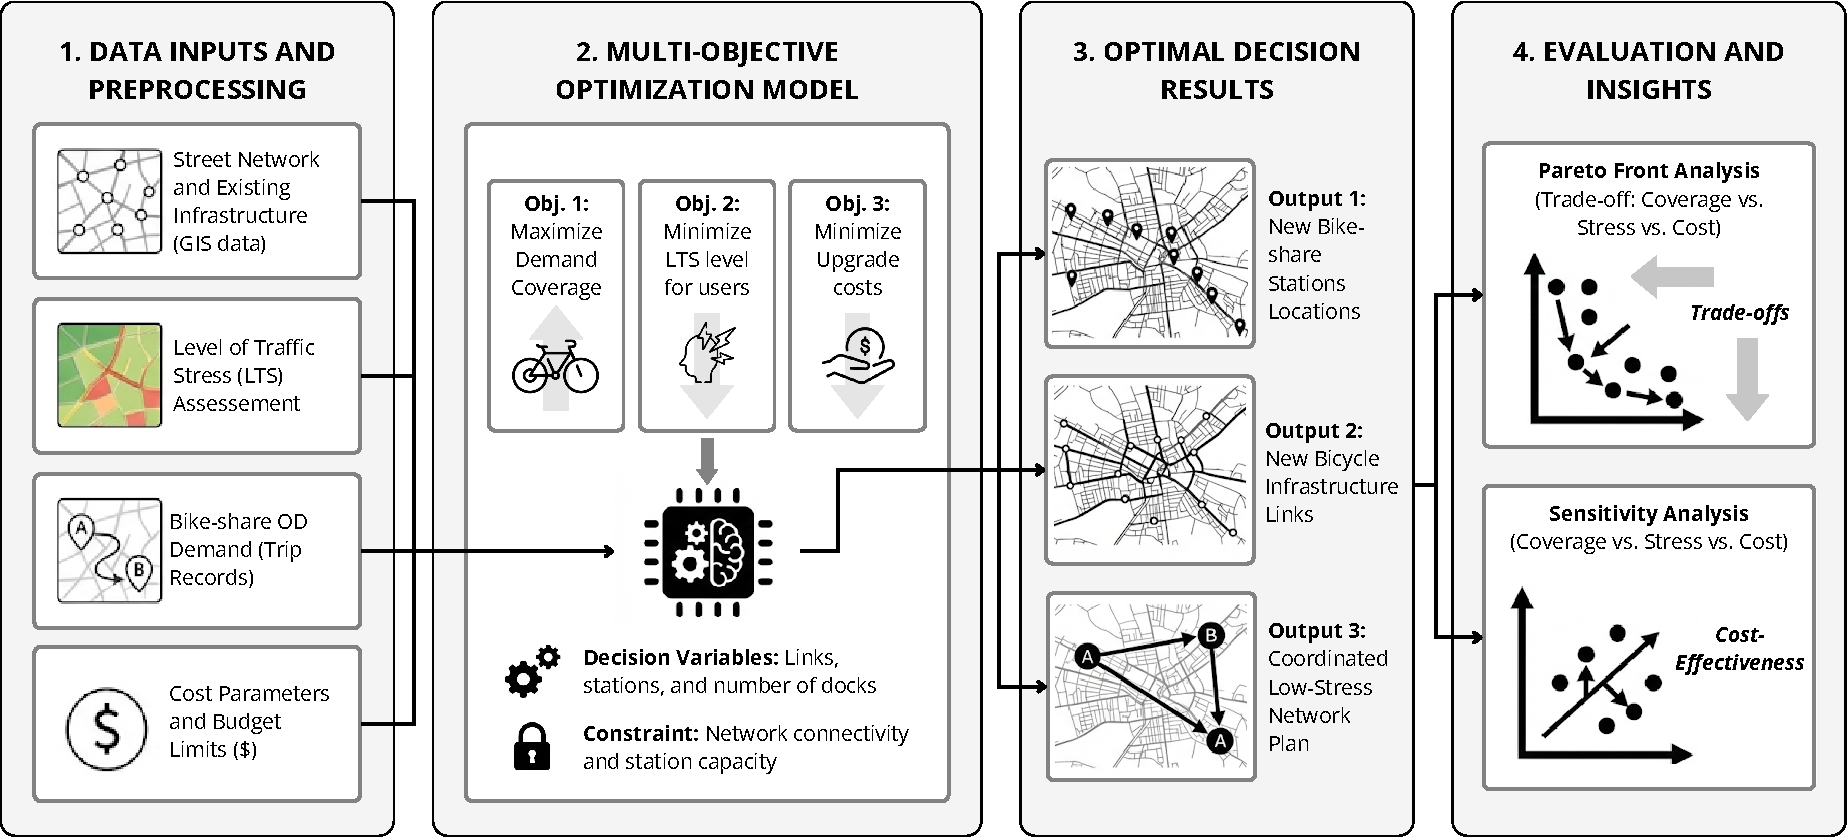
\includegraphics[width=1\textwidth]{Figures/framework.pdf}
  \caption{Framework applied in this paper.}\label{framework}
\end{figure}

The proposed methodology provides a systematic and integrated workflow for bicycle infrastructure planning. \textbf{(i) Data processing:} We compile, clean, and harmonize the inputs required by the model, including OD-based cycling demand estimates, station attributes, candidate locations, and geospatial network layers. \textbf{(ii) LTS classification:} We classify street segments according to traffic stress using speed, volume, lane, and bicycle-infrastructure attributes, producing the comfort metric used by the optimization model. \textbf{(iii) Optimization model:} We formulate a multi-objective MILP that co-optimizes bikeway upgrades and station-based supply by maximizing demand coverage while minimizing network-wide traffic stress and procurement costs, subject to operational and budget constraints; NSGA-II is then employed to approximate the Pareto-efficient solution set. \textbf{(iv) Environmental and modal-shift KPIs:} Each Pareto solution is post-processed to estimate potential avoided vehicle-kilometres and CO$_2$ emissions under transparent substitution assumptions. \textbf{(v) Velora platform:} The analytical workflow is implemented in a decision-support platform that supports data upload, scenario configuration, interactive comparison, saved runs, and automatic report generation.

Together, these steps provide actionable guidance by identifying cost-effective interventions that improve network usability, service coverage, and environmental performance. The remainder of this section details each component of the methodological approach, while the appendix provides additional platform screenshots and implementation details.

\subsection{Data Processing}

The data acquisition process involved integrating multiple sources to support both the demand modeling and infrastructure assessment components of this study. We collected detailed spatial and trip-level datasets to characterize the current cycling network and inform the development of the optimization model. These datasets were cleaned and processed to ensure compatibility across the analysis. Two primary inputs, namely cycling OD demand and LTS, formed the basis for constructing a realistic infrastructure planning framework.

%\subsubsection{Cycling Demand Acquisition}

Cycling demand is a key input to the proposed optimization framework because both station deployment and bikeway upgrades should reflect trip origins and destinations. To quantify this demand, we used the publicly available trip-level records from Montreal’s BIXI open data\footnote{More at: \url{https://bixi.com/en/open-data/}}, which report daily origin and destination stations, timestamps, and other relevant trip attributes. Figure \ref{fig:bixi_examples} illustrates a typical BIXI station and the spatial footprint of the current station network.

\begin{figure}[htbp]
    \centering
    \begin{subfigure}[b]{0.48\textwidth}
        \centering
        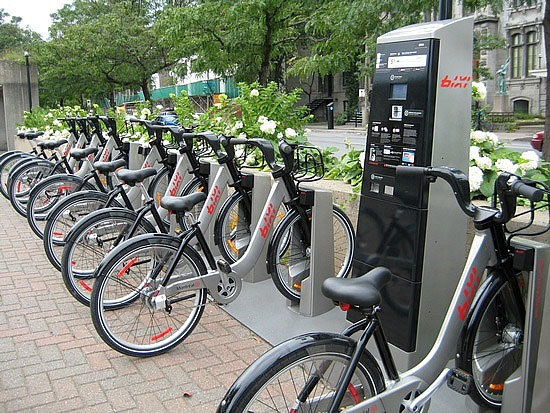
\includegraphics[width=\textwidth]{Figures/Bikesharing-BIXI-in-Montreal-see-online-version-for-colours.png}
        \caption{BIXI station with parked bicycles.}
        \label{fig:bixi_station}
    \end{subfigure}
    \hfill
    \begin{subfigure}[b]{0.425\textwidth}
        \centering
        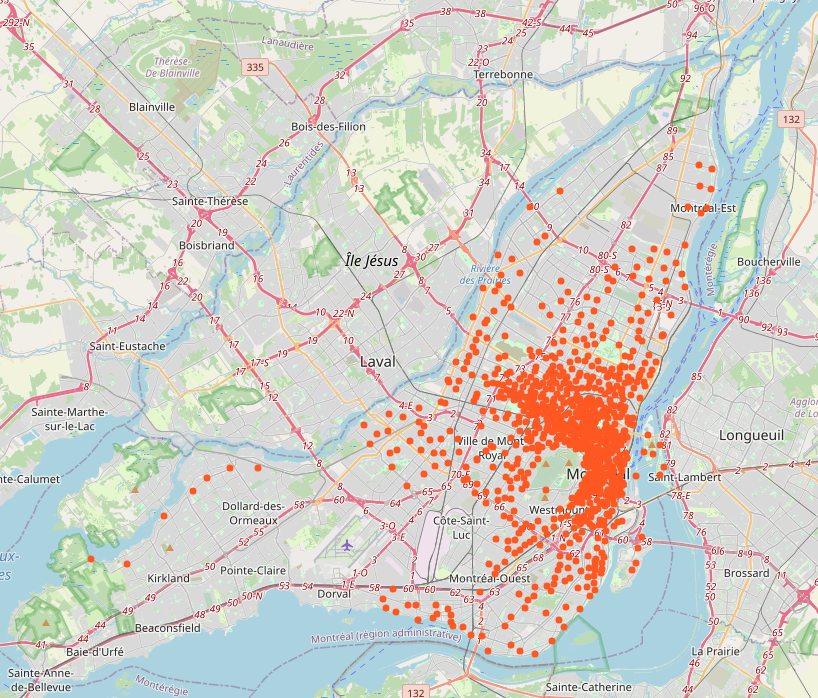
\includegraphics[width=\textwidth]{Figures/BIXI_Stations.png}
        \caption{Map of BIXI stations.}
        \label{fig:bixi_map}
    \end{subfigure}
    \caption{Illustrative examples of Montreal’s BIXI bike-sharing system.}
    \label{fig:bixi_examples}
\end{figure}

We extracted and processed OD trip records spanning multiple months of system operation and aggregated inbound and outbound activity at each station to construct a spatial demand surface. To link observed demand to candidate station locations in the optimization model, we defined service catchments around each station using circular buffers. A radius of 400~m was adopted, consistent with commonly used access distances in the bike-sharing literature \citep{el2017effects}. Demand within each catchment was computed by summing the numbers of trip origins and destinations associated with stations within the buffer, yielding a zonal estimate of cycling activity directly compatible with the candidate infrastructure graph.

Prior to aggregation, the dataset was cleaned to remove incomplete or implausible records, including trips with missing timestamps, invalid station identifiers, or zero duration. Station metadata was inferred by extracting unique station entries from the trip data. The resulting station-level demand estimates were then used to parameterize the optimization problem, ensuring that selected stations and upgraded links prioritize locations with demonstrated usage intensity and reflect observed travel behavior in the Montreal bike-sharing system.


\subsection{Level of Traffic Stress}\label{subsec:lts}

LTS classifies road segments and intersections into discrete stress levels based on operational and geometric characteristics, including motor-vehicle speed, traffic volume, number of travel lanes, and the presence and type of cycling infrastructure. This rider-centered approach is particularly relevant for cities aiming to increase mass cycling by attracting the large population segment characterized as \textit{interested but concerned} (Geller, 2006), rather than designing exclusively for confident riders. LTS thus provides an interpretable basis for identifying corridors likely to discourage stress-sensitive users and for prioritizing infrastructure upgrades that improve network usability and inclusivity.

\subsubsection{LTS Framework and Classification}\label{subsubsec:lts_definition}

The LTS framework classifies each road segment into one of four stress levels reflecting the tolerance of different cyclist groups. LTS~1 represents conditions suitable for all ages and abilities, while LTS~4 represents conditions appropriate only for very confident riders (see Figure \ref{fig:lts_levels}). This classification is grounded in empirical research on cyclist comfort and behavioral response to traffic stress (Mekuria et al., 2012; Furth et al., 2016) and has become standard in cycling network planning practice.

\begin{figure}[htb]
    \centering
    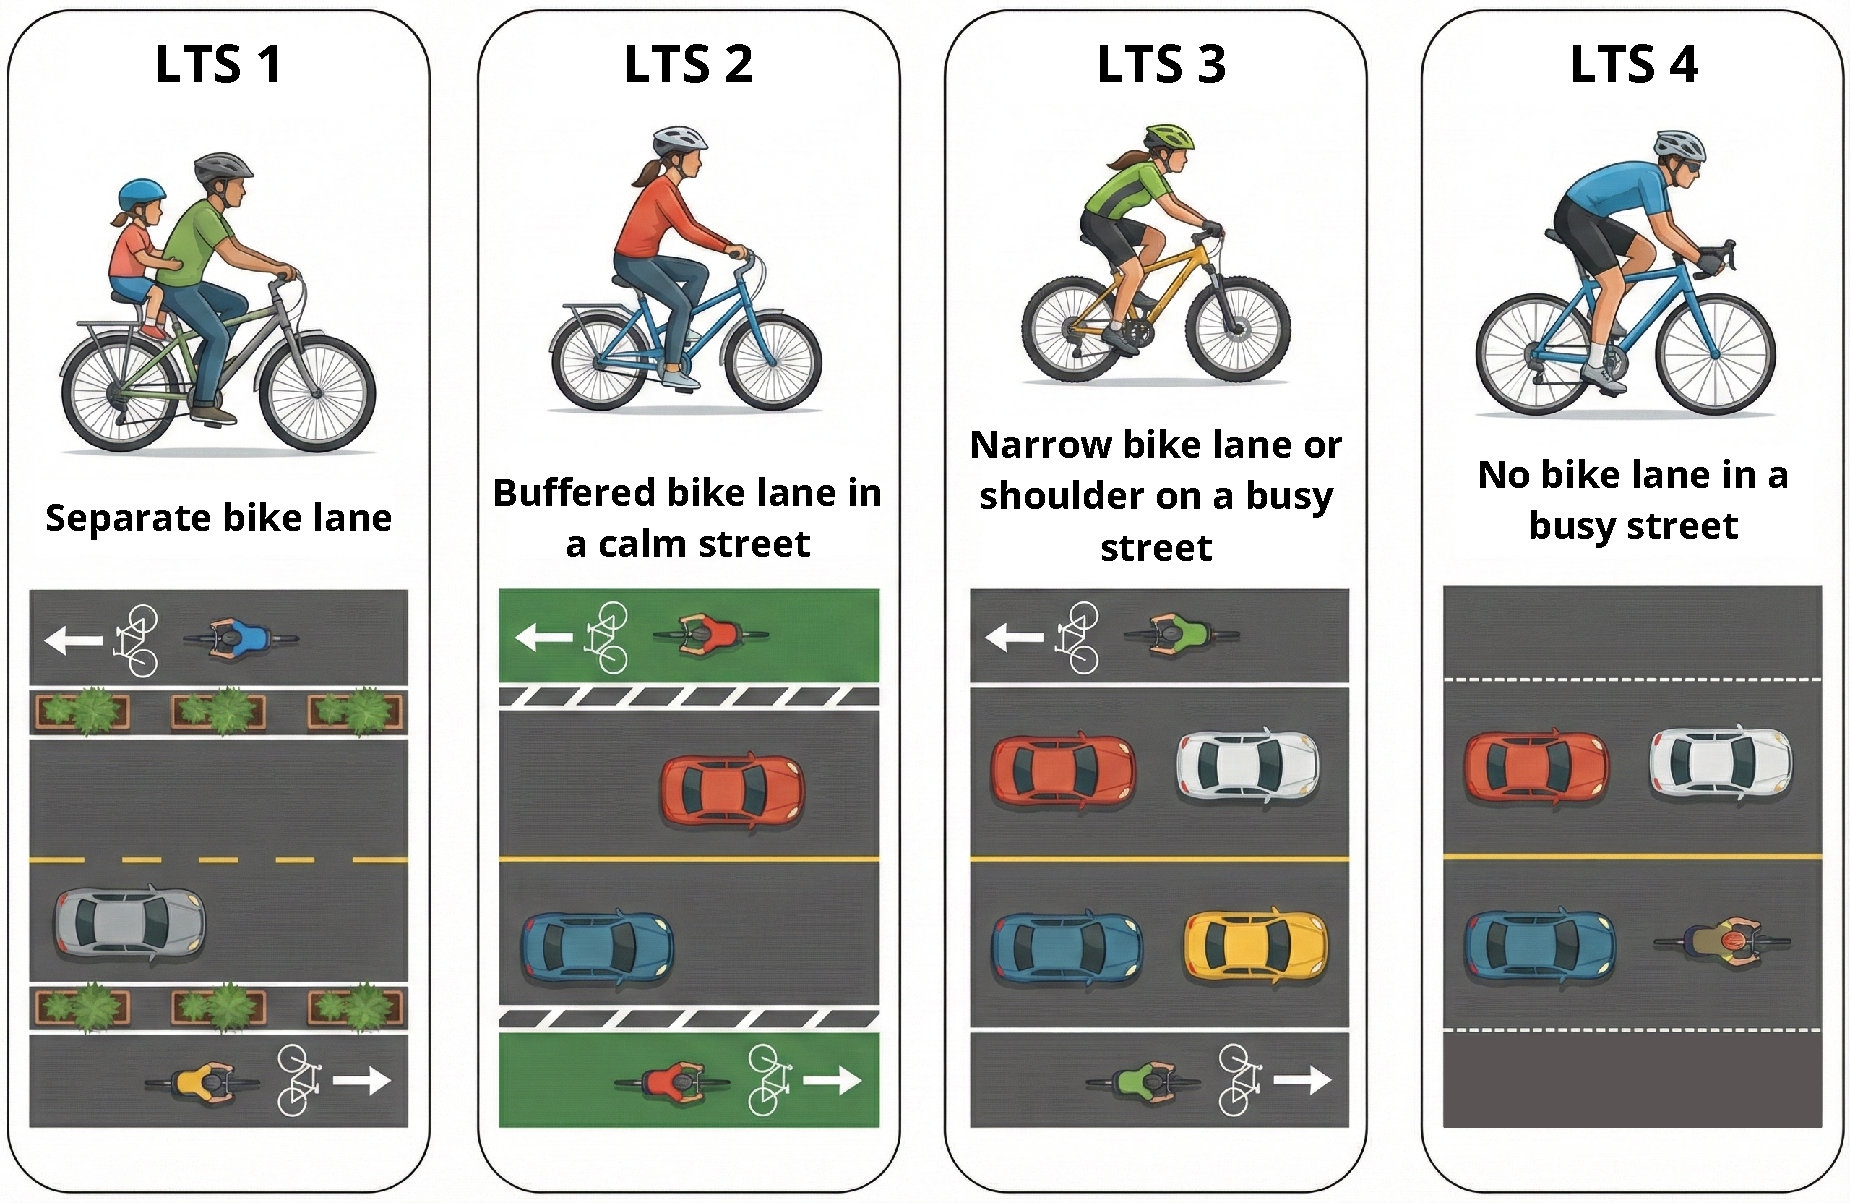
\includegraphics[width=1.0\textwidth]{Figures/lts.pdf}
    \caption{Illustration of the four LTS levels, from LTS~1 (all ages and abilities) to LTS~4 (very confident riders only).}
    \label{fig:lts_levels}
\end{figure}

The LTS classification is determined by evaluating four primary criteria: motor-vehicle speed, traffic volume, number of travel lanes, and bicycle infrastructure type and quality. Table~\ref{tab:lts_criteria} summarizes the evaluation thresholds for each LTS level. The framework prioritizes direct measures of speed and volume over functional-class proxies, as functional classes may misrepresent actual conditions---for example, a local street may carry several thousand vehicles per day in urban contexts, generating substantial stress despite its nominal classification. Recent refinements to the LTS framework (e.g., LTS~v2.0 and later versions) have improved representation of low-speed, high-volume streets and mixed-traffic conditions, addressing limitations that arise when applying the framework in large urban areas.

\begin{table}[htbp]
    \centering
    \small
    \caption{LTS evaluation criteria.}
    \label{tab:lts_criteria}
    \begin{tabularx}{\textwidth}{@{} l l l l l X @{}}
        \hline
        \textbf{LTS} & \textbf{Target Users} & \textbf{Speed} & \textbf{Volume} & \textbf{Lanes} & \textbf{Infrastructure} \\
        \hline
        1 & All ages and abilities & $\leq 40$ km/h & Low & $\leq 1$/direction & Separated facilities or quiet streets \\
        2 & Most adults, not children & $\leq 50$ km/h & Moderate & $\leq 2$/direction & Protected or painted bike lanes \\
        3 & Experienced cyclists & $\leq 60$ km/h & High & Multiple & Shared lanes, minimal facilities \\
        4 & Very confident cyclists & $> 60$ km/h & Very high & Multiple & No infrastructure, arterials \\
        \hline
    \end{tabularx}
\end{table}

\subsubsection{LTS Measurement and Mapping for Montreal}\label{subsubsec:lts_montreal}
 
Implementing network-wide LTS mapping requires overcoming a fundamental data challenge: obtaining reliable, spatially complete measures of traffic speed and volume across the entire study area. Functional-class proxies prove insufficient in urban contexts, where streets nominally classified as local may carry several thousand vehicles per day. To produce an LTS classification that reflects actual traffic conditions, we implemented a three-step, data-driven methodology combining empirical data sources, targeted validation, and automated classification. Figure \ref{fig:lts_framework} summarizes the framework.

\begin{figure}[htbp]
    \centering
    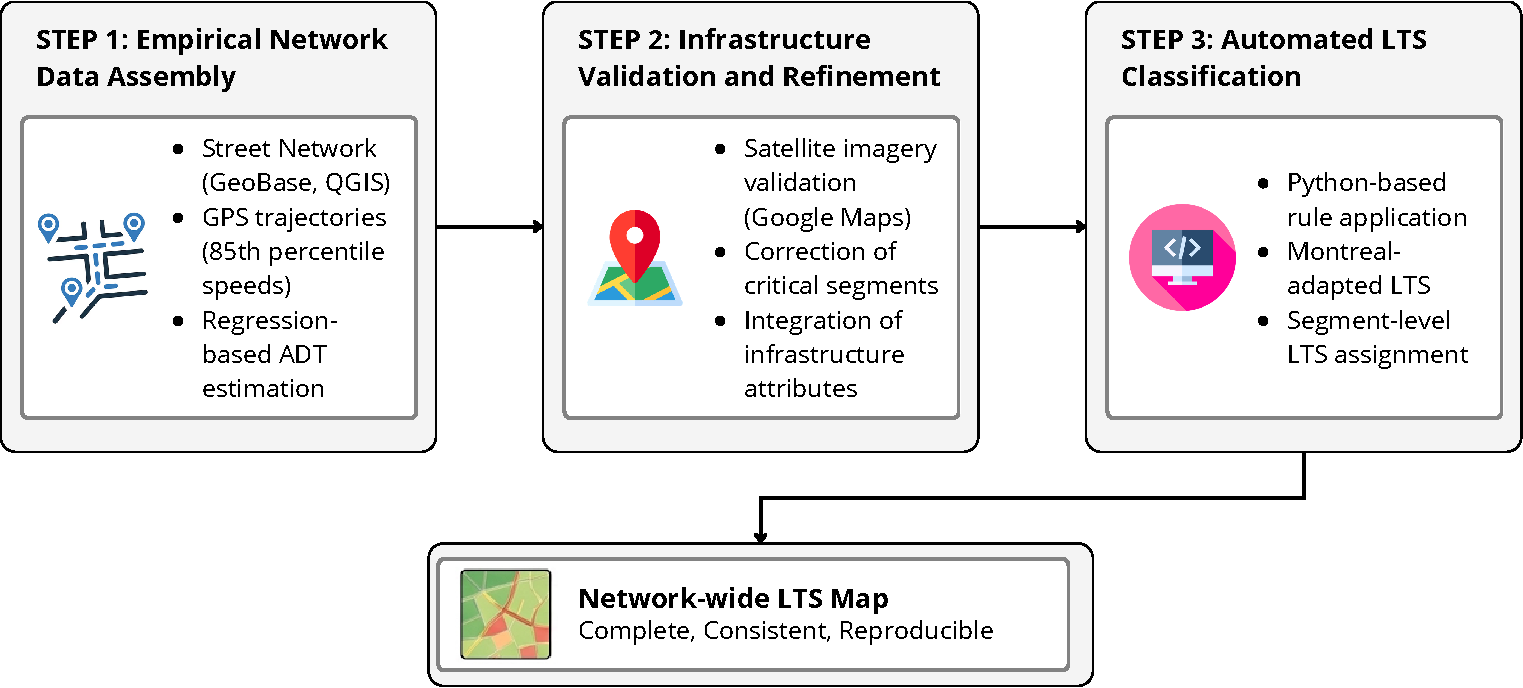
\includegraphics[width=1\linewidth]{Figures/lts_framework.pdf}
    \caption{LTS calculation framework.}
    \label{fig:lts_framework}
\end{figure}

This three-step approach (empirical data assembly, strategic validation, and transparent, automated classification) produced a network-wide LTS mapping that is comprehensive, defensible, and reproducible. In the following, we detail each step:

\textbf{Step 1 -- Network Assembly and Empirical Speed and Volume Data:} We began by constructing a street-segment network for the Island of Montreal in QGIS, using the City of Montreal's GeoBase as the foundation. Rather than inferring speed and volume from functional class, these variables were derived from empirical data. Where direct traffic counts and speed measurements were unavailable, full spatial coverage was achieved using large-scale GPS trajectory data (myDrive, Intact Insurance). Off-peak 85th-percentile vehicle speeds were computed for each segment to represent typical conditions without transient congestion. Average Daily Traffic (ADT) was estimated using regression models calibrated to observed traffic counts and adjusted for functional class, number of lanes, and one-way operation. This approach ensures that estimates remain grounded in observed traffic patterns rather than synthetic assumptions.
 
The resulting speed and volume distributions (Figure~\ref{fig:lts_measure_montreal}) reveal substantial spatial heterogeneity across Montreal. Figure~\ref{fig:lts_speed} shows that high speeds concentrate on arterial corridors while residential neighborhoods maintain lower speeds. Figure~\ref{fig:lts_traffic} illustrates that traffic volumes concentrate heavily downtown while peripheral areas see far less traffic. Critically, these maps reveal the limitation of functional-class assumptions: many ``local'' streets in central Montreal carry thousands of vehicles daily, while some secondary streets exhibit unexpectedly high speeds. A classification based solely on road type would misclassify stress conditions on numerous streets; direct measurement is essential for accuracy.
 
\begin{figure}[htbp]
    \centering
    \begin{subfigure}[t]{0.9\linewidth}
        \centering
        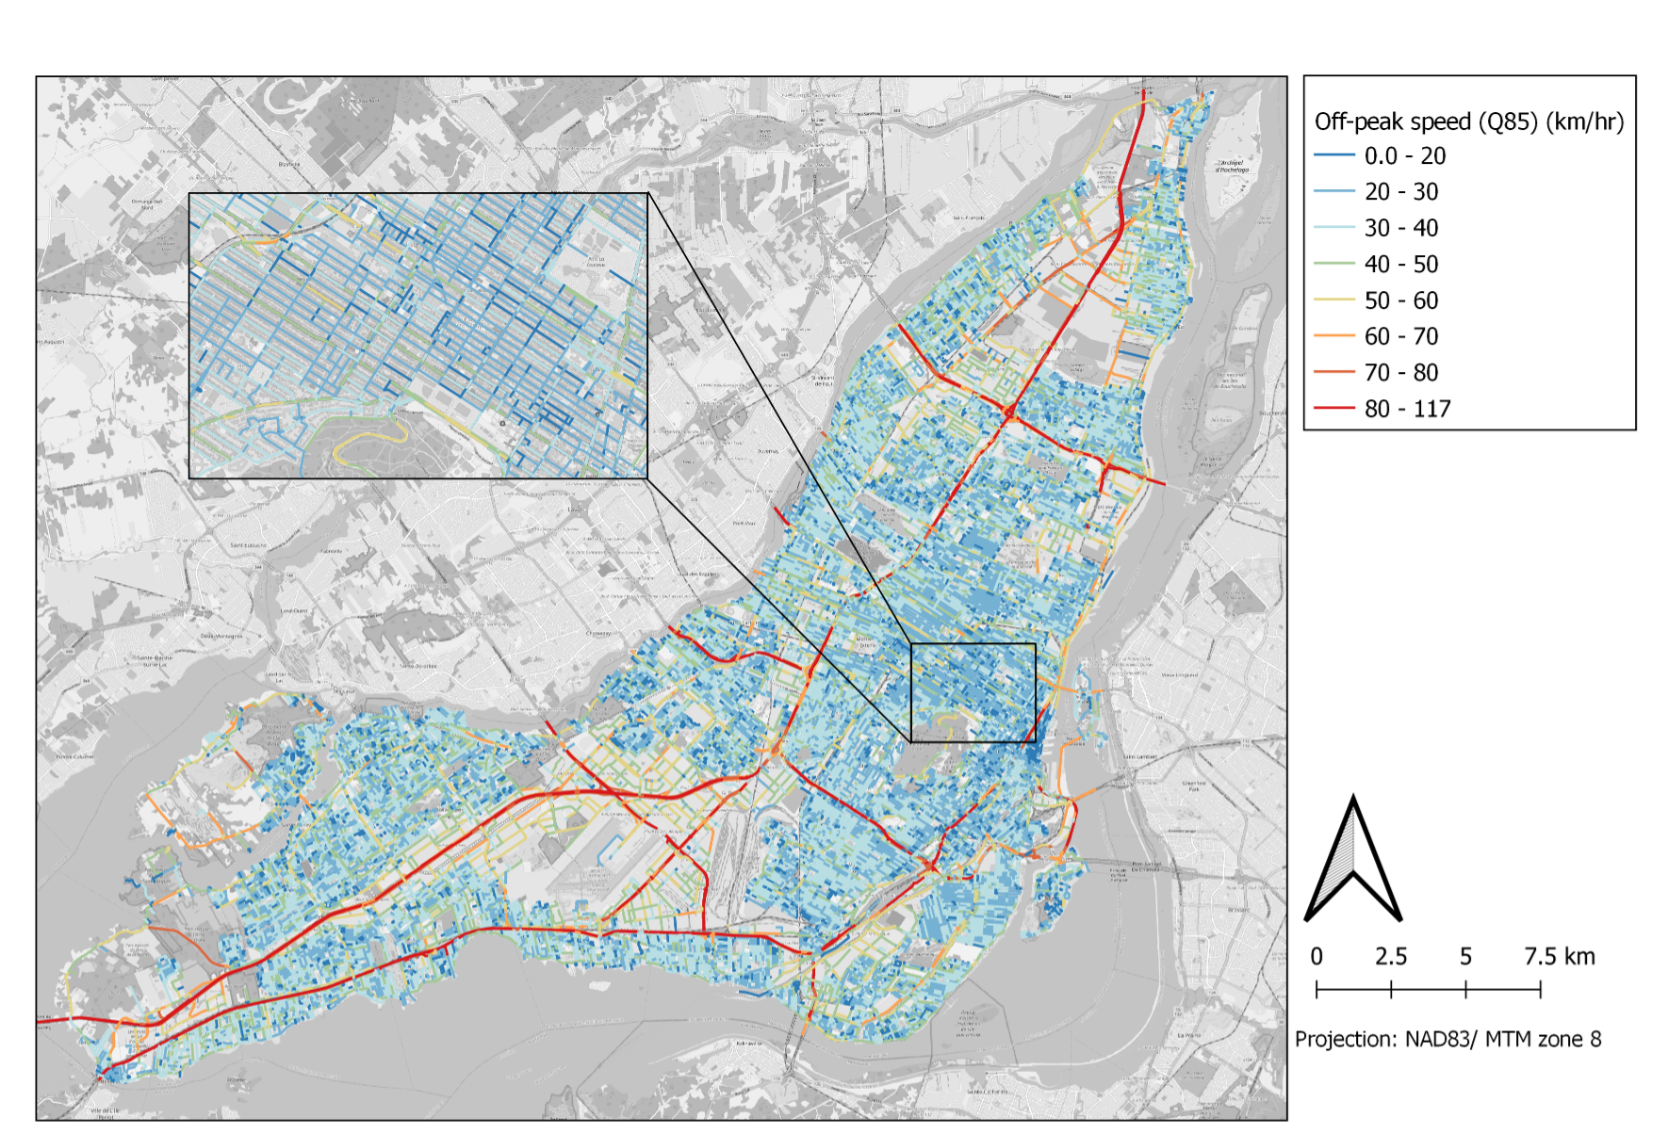
\includegraphics[width=\linewidth]{Figures/LTS_SpeedMeasures_link level.png}
        \caption{Off-peak 85th-percentile vehicle speeds.}
        \label{fig:lts_speed}
    \end{subfigure}
    \hfill
    \begin{subfigure}[t]{0.9\linewidth}
        \centering
        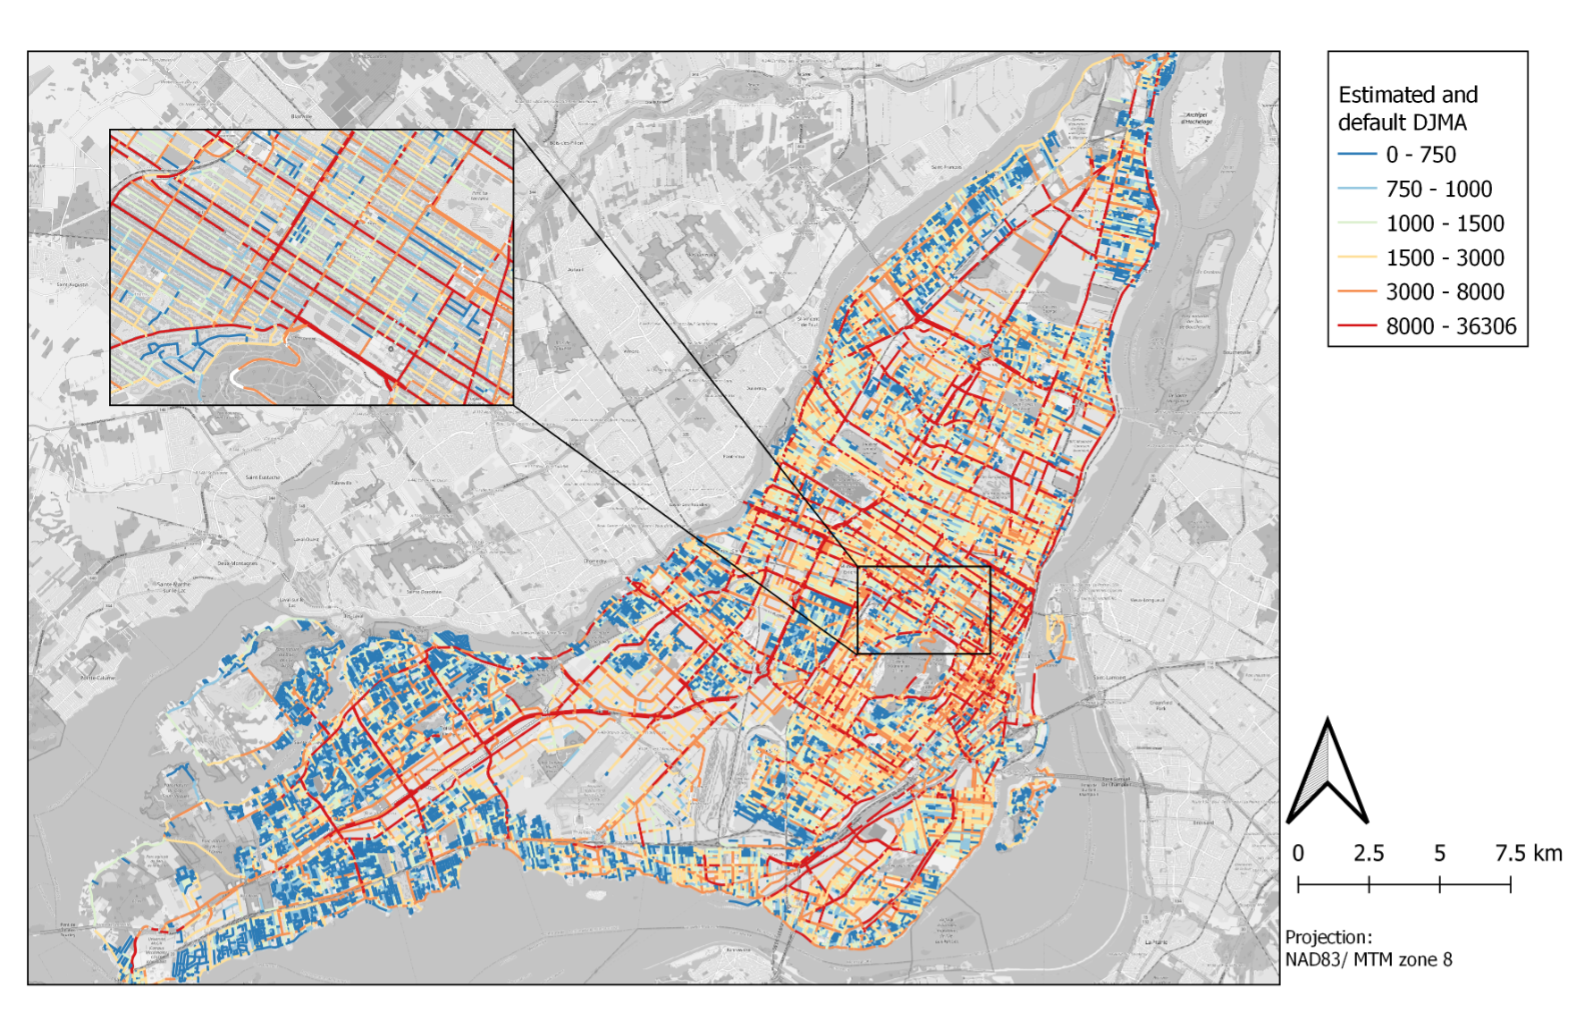
\includegraphics[width=\linewidth]{Figures/LTS_TrafficVolume_link level.png}
        \caption{Estimated traffic volume (ADT).}
        \label{fig:lts_traffic}
    \end{subfigure}
    \caption{Speed and volume distributions for Step 1: (a) off-peak vehicle speeds (85th-percentile) from GPS trajectories and (b) estimated traffic volumes (ADT) from regression models calibrated to observed traffic counts.}
    \label{fig:lts_measure_montreal}
\end{figure}
 
\textbf{Step 2 -- Infrastructure Validation and Refinement:} While speed and volume form the primary LTS classification inputs, bicycle infrastructure characteristics (lane width, continuity, separation from traffic, and centerline markings) also affect classification thresholds, particularly for painted bike lanes and mixed-traffic streets. Administrative datasets often encode these attributes inconsistently or incompletely. Rather than assuming the accuracy of administrative data, we conducted targeted validation using Google Maps satellite imagery. We identified segments that likely constitute classification exceptions (e.g., high-volume streets with newly constructed protective facilities or low-speed streets with inadequate infrastructure) and visually verified these critical segments. This strategic validation approach corrected the most consequential errors without requiring exhaustive inspection of every street, balancing accuracy against data-collection effort. We then consolidated all attributes (speed, volume, infrastructure, and geometric properties) into a unified geospatial database.
 
\textbf{Step 3 -- Automated LTS Classification:} In the final step, custom Python scripts applied LTS decision rules (Table~\ref{tab:lts_criteria}) to all network segments, using Montreal-specific parameters adapted from the LTS v2.0 framework. Automation ensures consistent application of classification logic across the entire network, eliminating manual inconsistencies and providing full transparency in decision-making. Each street segment is assigned a definitive LTS value, enabling its integration into the optimization model. 

\subsection{Optimization Model}\label{subsec:optimization_model}

This section presents the mathematical formulation and solution algorithm used to generate candidate infrastructure plans. The model defines the decision space, objectives, and feasibility constraints, while NSGA-II is used to approximate the Pareto front and expose trade-offs among demand coverage, traffic stress, and investment cost.

\subsubsection{Multi-Objective Mathematical Model}\label{subsubsec:math_model}

The proposed formulation is a tri-objective MILP that supports coordinated planning of bikeway upgrades and station-based bike-sharing supply. The model operates on a candidate graph $G=(N,L)$, where nodes $i\in N$ represent candidate station locations and edges $(i,j)\in L$ represent candidate bikeway links that can be upgraded and included in the final network. The decision variables select which stations to activate ($y_i$), which links to include ($x_{ij}$), and how much capacity (e.g., docks) to allocate at each active station ($z_i$). The complete nomenclature of the model is presented in Table \ref{tab:notation}.

\begin{table}[!ht]
\caption{Notation and Definitions.}
\label{tab:notation}
\centering
\small
\begin{tabularx}{0.85\textwidth}{@{} l l X @{}}
\hline
\textbf{Category} & \textbf{Symbol} & \textbf{Definition} \\
\hline

\multicolumn{3}{l}{\textit{Sets and Indices}} \\
& $N$ & Set of candidate bicycle stations, indexed by $i,j \in N$. \\
& $L \subseteq N \times N$ & Set of candidate bicycle network links, indexed by $(i,j)\in L$. \\
\hline

\multicolumn{3}{l}{\textit{Parameters}} \\
& $D_i$ & Potential cycling demand associated with station $i$ [trips], $i\in N$. \\
& $D_i^{peak}$ & Daily peak-demand at station $i$ for docks sizing [trips], $i\in N$. \\
& $LTS_{ij}$ & Level of Traffic Stress on link $(i,j)$, $(i,j)\in L$. \\
& $C_{ij}^{up}$ & Upgrade investment for link $(i,j)$ [CAD\$], if selected. \\
& $C^{dock}$ & Unit cost of a dock [CAD\$/unit], $i\in N$. \\
& $D^{\min}$ & Minimum total demand to be covered [trips]. \\
& $S^{\min}$ & Minimum number of stations to activate. \\
& $M^{\min}$ & Minimum number of links to activate. \\
& $\alpha,\beta,\gamma$ & Weights used in the scalarized objective function. \\
\hline

\multicolumn{3}{l}{\textit{Decision Variables}} \\
& $x_{ij}\in\{0,1\}$ & 1 if link $(i,j)\in L$ is selected, 0 otherwise. \\
& $y_i\in\{0,1\}$ & 1 if station $i\in N$ is activated, 0 otherwise. \\
& $z_i \ge 0$ & Capacity allocated at station $i$ (number of docks), $i\in N$. \\
\hline
\end{tabularx}
\end{table}


\begin{align}
\label{obj1_new}
Z_1 &= \text{Maximize} \sum_{i \in N} D_i\, y_i \\
\label{obj2_new}
Z_2 &= \text{Minimize} \sum_{(i,j) \in L} LTS_{ij}\, x_{ij} \\
\label{obj3_new}
Z_3 &= \text{Minimize} \sum_{(i,j)\in L} C_{ij}^{up}\, x_{ij} \;+\; \sum_{i\in N} C^{dock}\, z_i
\end{align}

Three competing objectives are considered. The first objective $Z_1$ maximizes covered cycling demand by prioritizing activation of stations located in high-demand zones. The second objective $Z_2$ minimizes the total traffic stress exposure across the selected links using the LTS score as a proxy for perceived comfort and safety. The third objective, $Z_3$, captures investment requirements by combining link-upgrade and station-capacity costs. This explicitly accounts for the fact that achieving low-stress connectivity typically requires additional infrastructure investment, and that station deployments must be supported by adequate service capacity.

\begin{align}
\label{const2_new}
\sum_{i\in N} y_i &\ge S^{\min} \\
\label{const3_new}
\sum_{(i,j)\in L} x_{ij} &\ge M^{\min} \\
\label{const4_new}
\sum_{i\in N} D_i\, y_i &\ge D^{\min} \\
\label{const_cap}
z_i &\ge D_i^{peak}\, y_i \quad \forall i \in N \\
\label{const5_new}
x_{ij} &\le y_i \quad \forall (i,j)\in L \\
\label{const6_new}
x_{ij} &\le y_j \quad \forall (i,j)\in L \\
\label{const7_new}
y_k &\le \sum_{(i,j)\in L:\, i=k \text{ or } j=k} x_{ij} \quad \forall k\in N
\end{align}

The constraints enforce practical feasibility. Constraints \eqref{const2_new}--\eqref{const4_new} ensure that the solution meets minimum infrastructure and service requirements, namely a minimum number of activated stations, a minimum number of selected links, and a minimum level of covered demand. Constraint \eqref{const_cap} links station activation to a capacity requirement, forcing stations to be provisioned with sufficient docks (or capacity-units) to satisfy a peak demand proxy whenever they are selected. Constraints \eqref{const5_new} and \eqref{const6_new} enforce link--station consistency by preventing a link from being selected unless both of its endpoints are active. Finally, constraint \eqref{const7_new} prevents isolated stations by requiring that each active station be incident to at least one selected link, thereby promoting a connected, implementable design.

\subsubsection{Solution Algorithm: NSGA-II}\label{subsubsec:nsga2}

To approximate the Pareto-efficient (non-dominated) set and make trade-offs among demand coverage, comfort, and cost explicit, we apply the Non-dominated Sorting Genetic Algorithm II (NSGA-II) \citep{debFastElitistMultiobjective2002}. NSGA-II is a well-established evolutionary multi-objective optimizer that uses elitist selection, non-dominated sorting, and crowding-distance ranking to preserve solution diversity along the Pareto front. An overview of the procedure applied in this paper is shown in Figure \ref{fig:solution_algorithm}.

\begin{figure}[htb]
\centering
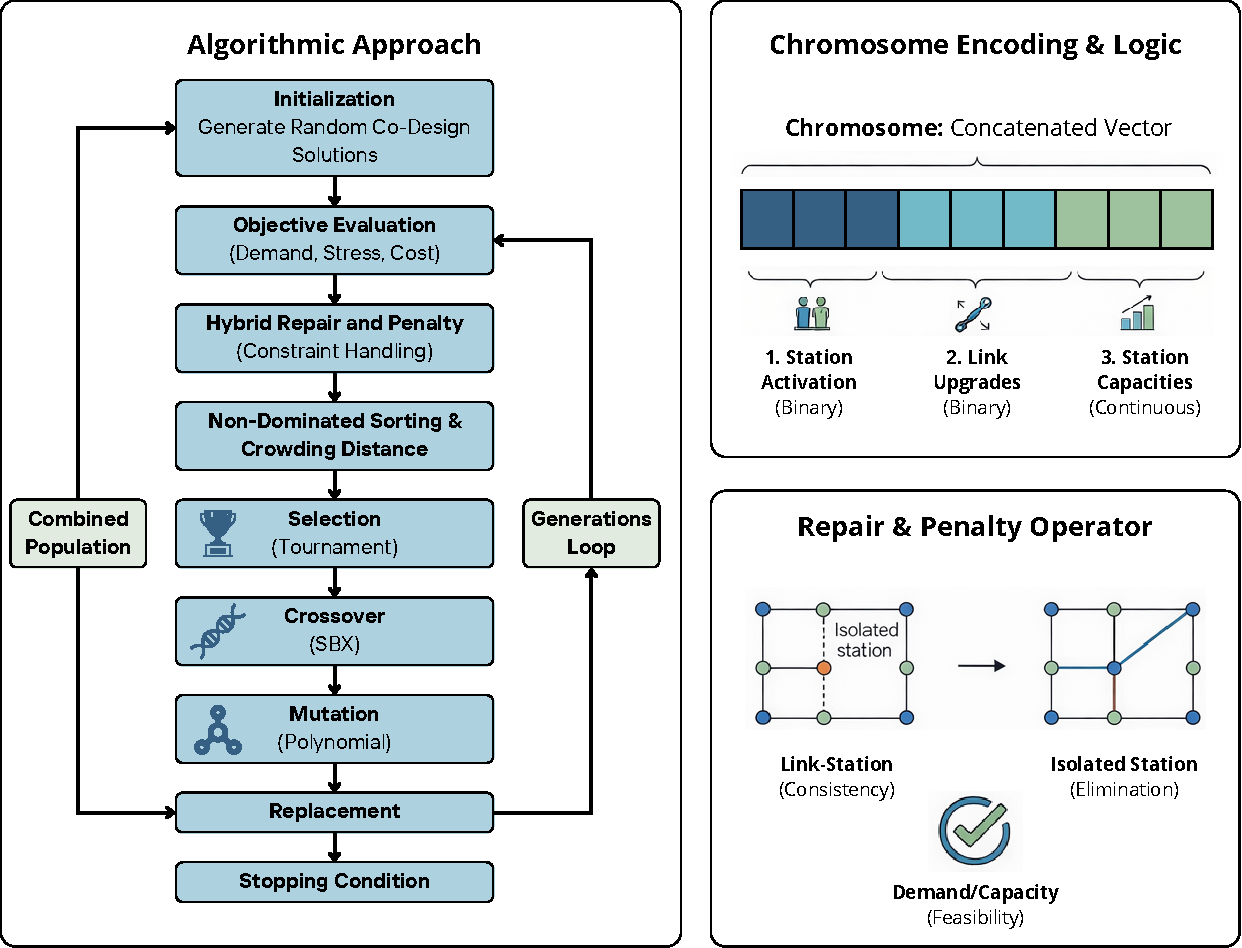
\includegraphics[width=1\textwidth]{Figures/ngsa_2.pdf}
\caption{Overview of the NSGA-II-based solution procedure for the integrated planning model.}
\label{fig:solution_algorithm}
\end{figure}

Given an initial population of candidate designs, NSGA-II iteratively improves solutions over generations using (i) objective evaluation, (ii) non-dominated sorting into Pareto fronts, (iii) diversity ranking via crowding distance, and (iv) variation operators (selection, crossover, mutation). At each generation, tournament selection favors solutions with better dominance rank and higher crowding distance. Offspring are generated through crossover and mutation, merged with the parent population, and then filtered via elitist replacement to form the next generation. The algorithm terminates after a predefined number of generations (or when improvement stagnates), returning a diverse approximation of the Pareto front that can be used to select representative designs for mapping and policy interpretation.

\textbf{Chromosome representation:} Each individual encodes a complete integrated plan with the same decision components as the MILP formulation: station activation, link selection for upgrade, and station capacity allocation. Specifically, the chromosome is defined as a concatenated vector:

\begin{equation}
\mathbf{g} \;=\; \big[\, \mathbf{y}\;|\;\mathbf{x}\;|\;\mathbf{z}\,\big],
\end{equation}

where $\mathbf{y}=\{y_i\}_{i\in N}$ are binary station activation variables, $\mathbf{x}=\{x_{ij}\}_{(i,j)\in L}$ are binary link selection variables, and $\mathbf{z}=\{z_i\}_{i\in N}$ are continuous nonnegative capacity variables. The chromosome dimension is therefore $2|N|+|L|$. This mixed encoding allows NSGA-II to explore joint decisions over network structure (stations and upgraded links) and operational feasibility (capacity) within a unified search space.

\textbf{Objective evaluation:} For each individual $\mathbf{g}$, objective values are computed using the definitions in Section~\ref{subsubsec:math_model}. In particular, the algorithm evaluates (i) total covered demand induced by activated stations, (ii) total stress exposure over selected links based on $LTS_{ij}$, and (iii) total procurement cost combining link upgrade costs and station capacity costs. The resulting objective vector is used for Pareto dominance comparisons during non-dominated sorting:

\begin{equation}
\mathbf{Z}(\mathbf{g}) \;=\; \big(Z_1(\mathbf{g}),\, Z_2(\mathbf{g}),\, Z_3(\mathbf{g})\big)
\end{equation}



\textbf{Constraint handling and feasibility:} Variation operators can produce infeasible solutions that violate the logical and operational constraints of the planning problem. We handle feasibility using a hybrid approach consisting of (i) a repair operator and (ii) a penalty mechanism for any remaining violations. The repair operator enforces the key structural constraints used in the MILP: (a) link--station consistency (a link can only be selected if both endpoint stations are active), (b) prevention of isolated activated stations (each active station must be incident to at least one selected link), and (c) capacity feasibility (active stations must satisfy the peak-demand proxy through $z_i \ge D_i^{peak}y_i$). After repair, any residual violation is quantified through a scalar constraint-violation function $V(\mathbf{g})\ge 0$. During selection and sorting, infeasible solutions are penalized such that feasible solutions dominate infeasible ones, and among infeasible designs, lower violation is preferred. This strategy preserves the exploratory benefits of evolutionary search while steering the population toward implementable infrastructure plans.

\textbf{Variation operators:} We use operators that match the mixed decision structure. Two-point crossover is applied to the concatenated chromosome, preserving contiguous blocks of decisions. Mutation is applied using bit-flip operators for the binary components ($\mathbf{y}$ and $\mathbf{x}$) and Gaussian perturbation for the continuous component ($\mathbf{z}$), followed by nonnegativity bounding and repair. This design allows both structural modifications (adding/removing stations or upgrading links) and fine-grained adjustments (capacity reallocation) within the same evolutionary cycle.

\textbf{Parameter settings and termination:} NSGA-II performance depends on algorithm settings that control exploration, exploitation, and runtime. In the computational experiments, we specify a population size, number of generations, crossover probability, and mutation probabilities for both binary and continuous components. The algorithm terminates after a fixed number of generations, and the final output is the non-dominated set from the terminal population, which serves as an approximation of the Pareto front. We subsequently select representative solutions (e.g., demand-oriented, comfort-oriented, cost-oriented, and compromise designs) for visualization and planning interpretation.

\subsection{Environmental and Modal-Shift KPIs}\label{subsec:environmental_kpis}

To adapt the optimization workflow to transport-environment appraisal, Velora post-processes each Pareto-efficient solution using modal-shift and avoided-emissions indicators. These indicators are not introduced as additional optimization objectives in the current application; rather, they provide a transparent policy-evaluation layer that converts served bike-share demand into potential reductions in motorized travel and tailpipe CO$_2$ emissions. This distinction is important because the environmental benefits of bike sharing depend strongly on which modes are replaced. Prior studies show that bike-share trips may substitute not only car trips, but also walking, personal cycling, and public transit \citep{fuller2013potential, RICCI201528, saltykova2022environmental}. Active-travel emissions studies and e-bike mode-shift assessments similarly show that climate benefits depend on avoided motorized travel and induced trip assumptions \citep{BRAND2021102764, MCQUEEN2020102482}. Therefore, Velora evaluates emissions benefits under explicit substitution assumptions rather than assuming that all served bicycle trips replace car travel.

Let $s\in S$ denote a candidate solution on the Pareto front and let $T_s$ be the number of annual trips served by solution $s$, corresponding to objective $Z_1$. Let $\bar{d}$ denote the average bike-share trip length in kilometres, and let $\rho_m$ represent the share of served bike-share trips that replace trips by mode $m\in M$, where $M$ may include car, taxi/ride-hailing, bus, metro, walking, or personal bicycle. Let $e_m$ be the emission factor for mode $m$ in kg CO$_2$ per passenger-km and $e_b$ be the operating emission factor of the bike-share trip. For conventional bicycles, $e_b$ is assumed to be zero at the point of use; life-cycle bicycle production, charging, and rebalancing emissions are excluded from the main calculation and should be added in future life-cycle extensions. The modal-shift and environmental KPIs are defined as:

\begin{equation}
\label{eq:avoided_pkm}
\Delta p_{s,m} = T_s \rho_m \bar{d}.
\end{equation}

For private automobiles, with $\omega_c$ denoting average vehicle occupancy:

\begin{equation}
\label{eq:avoided_vkt}
\Delta v_s = \frac{T_s \rho_c \bar{d}}{\omega_c}.
\end{equation}

The general and car-substitution emissions indicators are:

\begin{equation}
\label{eq:avoided_co2_general}
\Delta E_s = T_s \bar{d} \sum_{m\in M} \rho_m (e_m - e_b),
\end{equation}

\begin{equation}
\label{eq:avoided_co2_car}
\Delta E_{s,c} = T_s \rho_c \bar{d} e_c.
\end{equation}

Environmental cost-effectiveness is defined as:

\begin{equation}
\label{eq:co2_cost_effectiveness}
\eta_s = \frac{\Delta E_s/1000}{Z_{3,s}}.
\end{equation}

Here, $\Delta p_{s,m}$ is avoided passenger-kilometres by replaced mode, $\Delta v_s$ is avoided vehicle-kilometres for car substitution, $\Delta E_s$ is avoided CO$_2$ in kg/year, $\Delta E_{s,c}$ is the car-substitution special case, and $\eta_s$ is expressed in tonnes CO$_2$ avoided per CAD\$ million when $Z_{3,s}$ is reported in million CAD. For the illustrative analysis, we use $e_c=0.2485$ kg CO$_2$/km, derived from the U.S. EPA estimate that a typical passenger vehicle emits approximately 400 g CO$_2$ per mile \citep{epaTypicalVehicle2025}. We report the main results using $\bar{d}=2.0$ km, $\rho_c=5\%$, and $\omega_c=1$, while interpreting this as a scenario assumption rather than an observed modal-shift estimate. Sensitivity to $\rho_c$ is linear and can be evaluated directly using Equations~\eqref{eq:avoided_vkt}--\eqref{eq:avoided_co2_car}; for example, a 10\% car-substitution rate doubles the avoided VKT and CO$_2$ values reported below.

\subsection{Velora Platform Description}\label{subsec:velora_platform}

Velora translates the data-processing, LTS, optimization, and KPI workflow into a decision-support environment for planners, analysts, and policy stakeholders. Consistent with decision-support-system applications in cycling planning \citep{silvestriCyclabilityDSS2024}, the platform links a Streamlit front-end with a persistent analytical back-end. Users upload station-demand and LTS network layers, configure planning assumptions and NSGA-II parameters, run or reopen scenarios, compare Pareto-efficient alternatives through maps and metrics, export selected station and link outputs, and automatically generate city-ready reports. Figure~\ref{fig:velora_platform_workflow} summarizes this platform workflow. In the main manuscript, Velora is treated as the implementation layer that makes the method repeatable and communicable; Appendix~\ref{app:velora_platform} provides additional details on platform functioning, modules, user experience, screenshots, and implementation notes.

\begin{figure}[htbp]
  \centering
  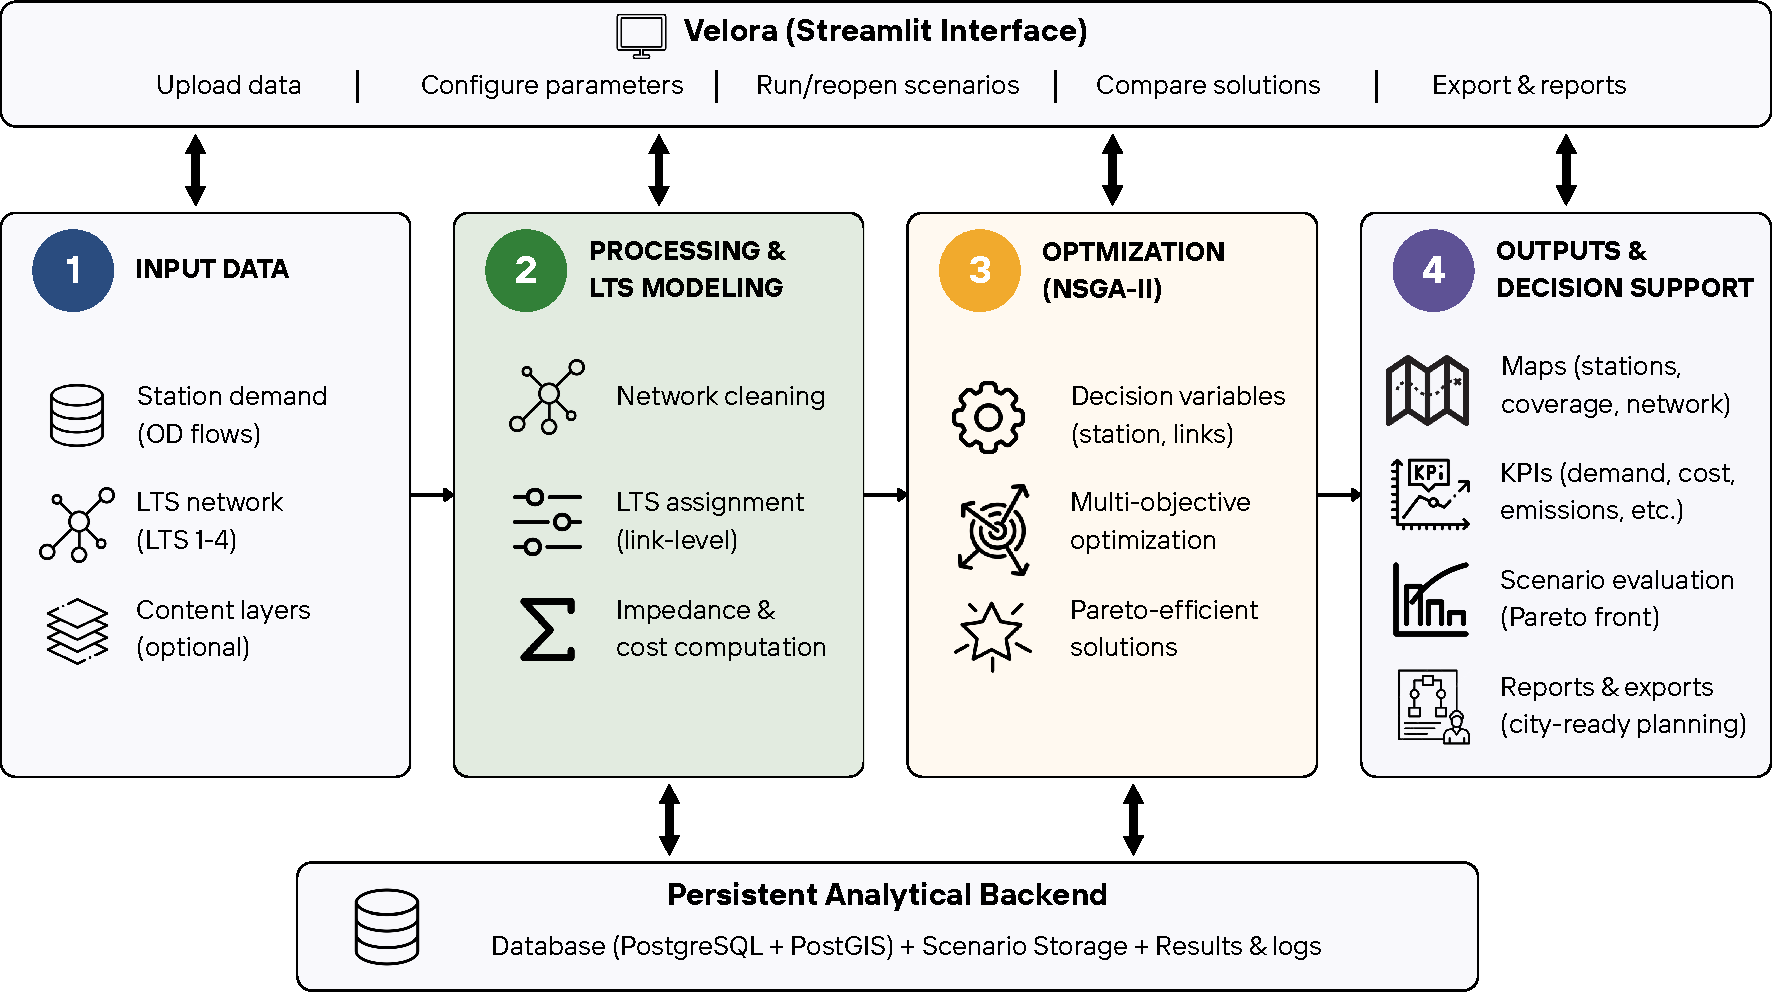
\includegraphics[width=\textwidth]{Figures/velora_platform_workflow.pdf}
  \caption{Velora platform workflow linking the Streamlit interface, input data, LTS processing, multi-objective optimization, outputs, decision support, and persistent analytical back-end.}
  \label{fig:velora_platform_workflow}
\end{figure}


% -------------------- Case Study --------------------


\section{Case Study Description}\label{casestudy}

Montreal offers an ideal setting for this study due to its large bike-sharing system and comprehensive data, which facilitate station and network optimization. The BIXI system records urban cycling demand, helping derive realistic station placement patterns. The street network includes various cycling facilities, allowing assessment of infrastructure comfort constraints on station configurations. This section details the demand patterns, candidate station location generation method, and the LTS mapping and parameters used in experiments.

\subsection{BIXI Demand Patterns and Candidate Station Locations}\label{subsec:bixi_demand}

The processed 2025 BIXI dataset includes 14,249,363 trips across 1,296 origin stations, providing a detailed empirical representation of urban cycling demand. Key summary statistics are reported in Table \ref{tab:bixi_data_summary}.

\begin{table}[htbp]
  \centering
  \caption{Summary statistics of the 2025 BIXI dataset used in this case study.}
  \label{tab:bixi_data_summary}
  \small
  \begin{tabularx}{0.82\textwidth}{@{} l X @{} }
    \hline
    \textbf{Indicator} & \textbf{Value} \\
    \hline
    Annual BIXI trips (2025) & 14,249,363 \\
    Distinct origin stations & 1,296 \\
    Share of origins in Le Plateau-Mont-Royal and Ville-Marie & 57.5\% \\
    Activity captured by top 30 stations & 3,508,845 trips \\
    Activity captured by top 10 stations & 1,553,726 trips \\
    Trips occurring from April to November & 97.6\% \\
    Trips occurring from June to September & 63.7\% \\
    \hline
  \end{tabularx}
\end{table}

Two structural features are particularly relevant for the optimization problem. First, demand is strongly centralized, with Le Plateau-Mont-Royal and Ville-Marie accounting for 57.5\% of trip origins, indicating a well-defined high-activity corridor. Second, usage is highly seasonal, with 97.6\% of trips occurring between April and November and 63.7\% during June to September, reflecting Montreal’s climatic constraints.

To focus the analysis on the most critical trade-offs between coverage, comfort, and investment, we consider the 30 highest-activity stations within the downtown cluster (Figure \ref{fig:bixi_demand_map}). These stations account for 3.51 million interactions, with the top 10 alone contributing 1.55 million, ensuring that the study area captures the most intensive portion of system demand. The full list of selected stations and their activity levels is provided in \ref{app:top30_stations}.

\begin{figure}[htbp]
    \centering
    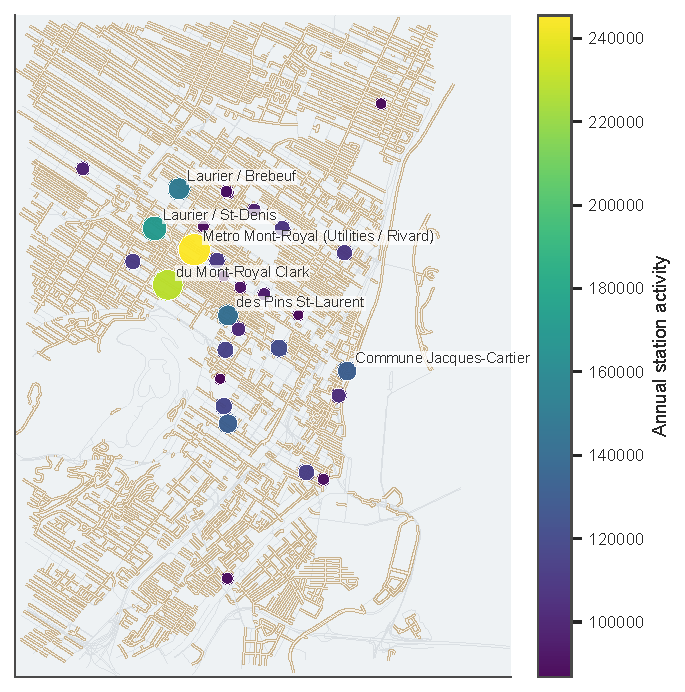
\includegraphics[width=0.72\textwidth]{Figures/BIXI_case_top30_station_map.pdf}
    \caption{Spatial distribution of the 30 highest-activity BIXI stations within the downtown study area.}
    \label{fig:bixi_demand_map}
\end{figure}

At a broader spatial scale, demand also clusters at the borough level. Figure~\ref{fig:bixi_borough_activity} shows origin and destination volumes across Montreal’s main boroughs. Le Plateau-Mont-Royal, Ville-Marie, and Rosemont--La Petite-Patrie dominate both, while neighboring boroughs exhibit directional imbalances. This pattern indicates that the downtown core operates as part of a larger central activity belt rather than an isolated demand center.

\begin{figure}[htbp]
    \centering
    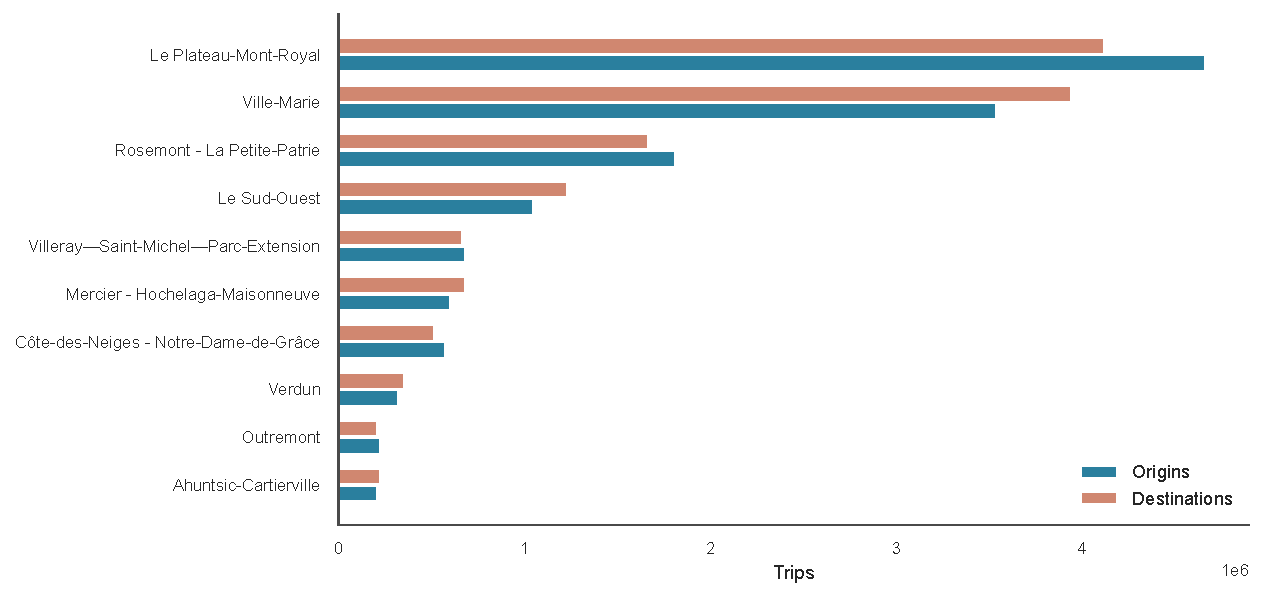
\includegraphics[width=0.80\textwidth]{Figures/BIXI_case_borough_activity.pdf}
    \caption{Origin and destination activity volumes across Montreal's boroughs.}
    \label{fig:bixi_borough_activity}
\end{figure}

\subsubsection{Temporal Demand Structure}

Beyond spatial patterns, BIXI demand exhibits strong temporal variation at multiple timescales. Understanding this temporal structure is essential for calibrating demand assumptions in the optimization model. Figure~\ref{fig:bixi_temporal_ab} shows complementary perspectives on demand timing at different temporal scales.

\begin{figure}[htbp]
    \centering
    \begin{subfigure}[t]{0.8\textwidth}
        \centering
        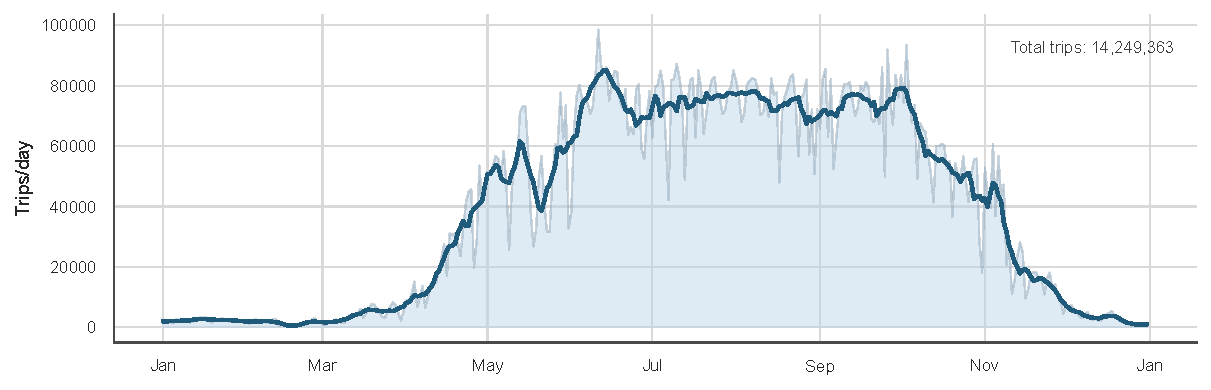
\includegraphics[width=\linewidth]{Figures/BIXI_case_daily_ridership.pdf}
        \caption{Daily ridership profile.}
        \label{fig:bixi_daily_profile}
    \end{subfigure}
    
    \vspace{0.4cm}
    
    \begin{subfigure}[t]{0.8\textwidth}
        \centering
        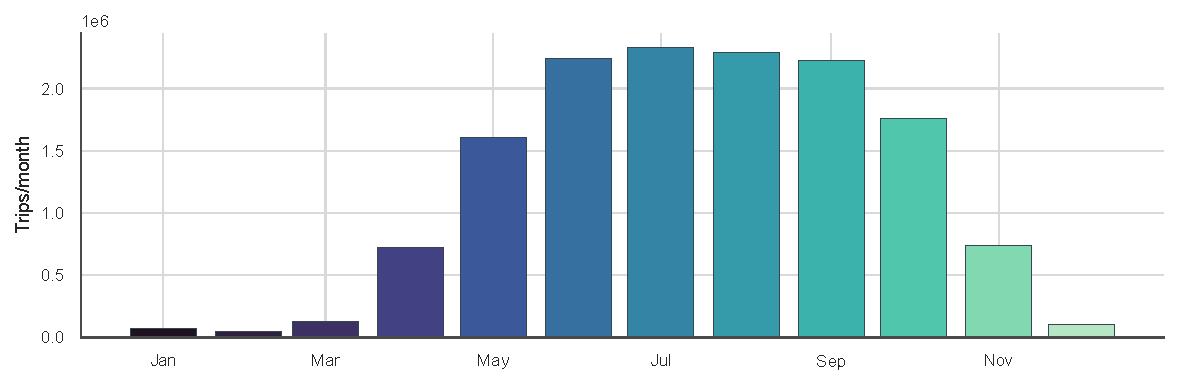
\includegraphics[width=\linewidth]{Figures/BIXI_case_monthly_ridership.pdf}
        \caption{Monthly ridership profile.}
        \label{fig:bixi_temporal_patterns}
    \end{subfigure}
    
    \caption{Temporal evolution of BIXI ridership in 2025 across (a) daily and (b) monthly scales.}
    \label{fig:bixi_temporal_ab}
\end{figure}

At the seasonal scale (Figure~\ref{fig:bixi_daily_profile}), ridership follows a pronounced annual cycle characterized by a rapid ramp-up beginning in spring, a sustained plateau during summer months, and a marked decline as fall arrives. This seasonality reflects Montreal's winter climate and demonstrates that BIXI functions primarily as a warm-season mobility option. At the sub-annual scale (Figure~\ref{fig:bixi_temporal_patterns}), ridership peaks in the months of June through September, which account for 63.7\% of annual trips. This concentration has important implications for planning: it suggests that infrastructure investments and station placement should prioritize serving peak-season demand, while recognizing that the system experiences reduced but non-trivial activity during shoulder months.

Figure~\ref{fig:bixi_weekly_profile} presents a heatmap of BIXI departures by day of week and hour of day, revealing a distinct weekly structure.

\begin{figure}[htbp]
    \centering
    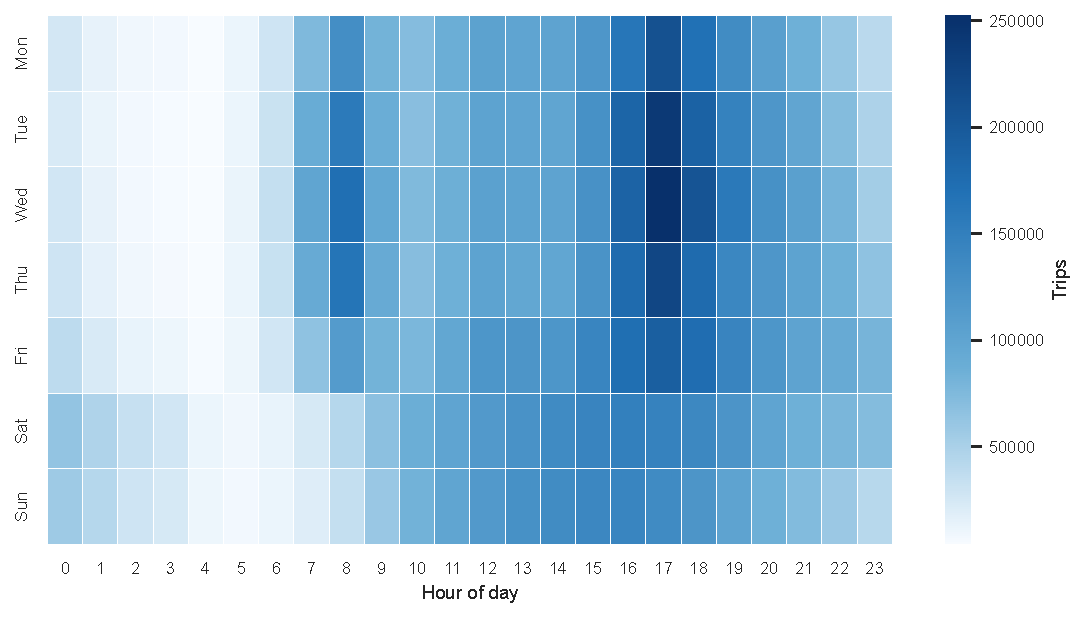
\includegraphics[width=0.75\textwidth]{Figures/BIXI_case_weekday_hour_heatmap.pdf}
    \caption{Weekly and hourly usage structure of BIXI departures in 2025.}
    \label{fig:bixi_weekly_profile}
\end{figure}

In the optimization framework, we use annual observed origin-destination demand as the planning baseline. This approach captures the full diversity of demand patterns while allowing the algorithm to identify station configurations that perform well across multiple temporal windows. The temporal concentrations documented above inform our interpretation of optimization results, allowing us to assess whether solutions prioritize peak-season performance or balance demand across seasons.

\subsubsection{Candidate Station Location Generation}

To allow station placement decisions to respond to comfort constraints, we generate multiple candidate locations for each existing station. For each of the 30 high-activity stations, we define a service buffer around the current location and generate five equidistant candidate sites within this buffer. This approach enables the optimization model to either retain an existing station's current location or relocate it to a nearby alternative site if doing so improves access to low-stress cycling infrastructure. For example, if a station's current location requires access via high-stress network segments, the algorithm may select an alternative candidate location that provides better integration with comfortable, low-stress facilities.

\subsection{Cycling Comfort and LTS Mapping}\label{subsec:lts_mapping}

Figure~\ref{fig:lts_mapping} visualizes the spatial distribution of LTS classifications across Montreal. 

\begin{figure}[htbp]
    \centering
    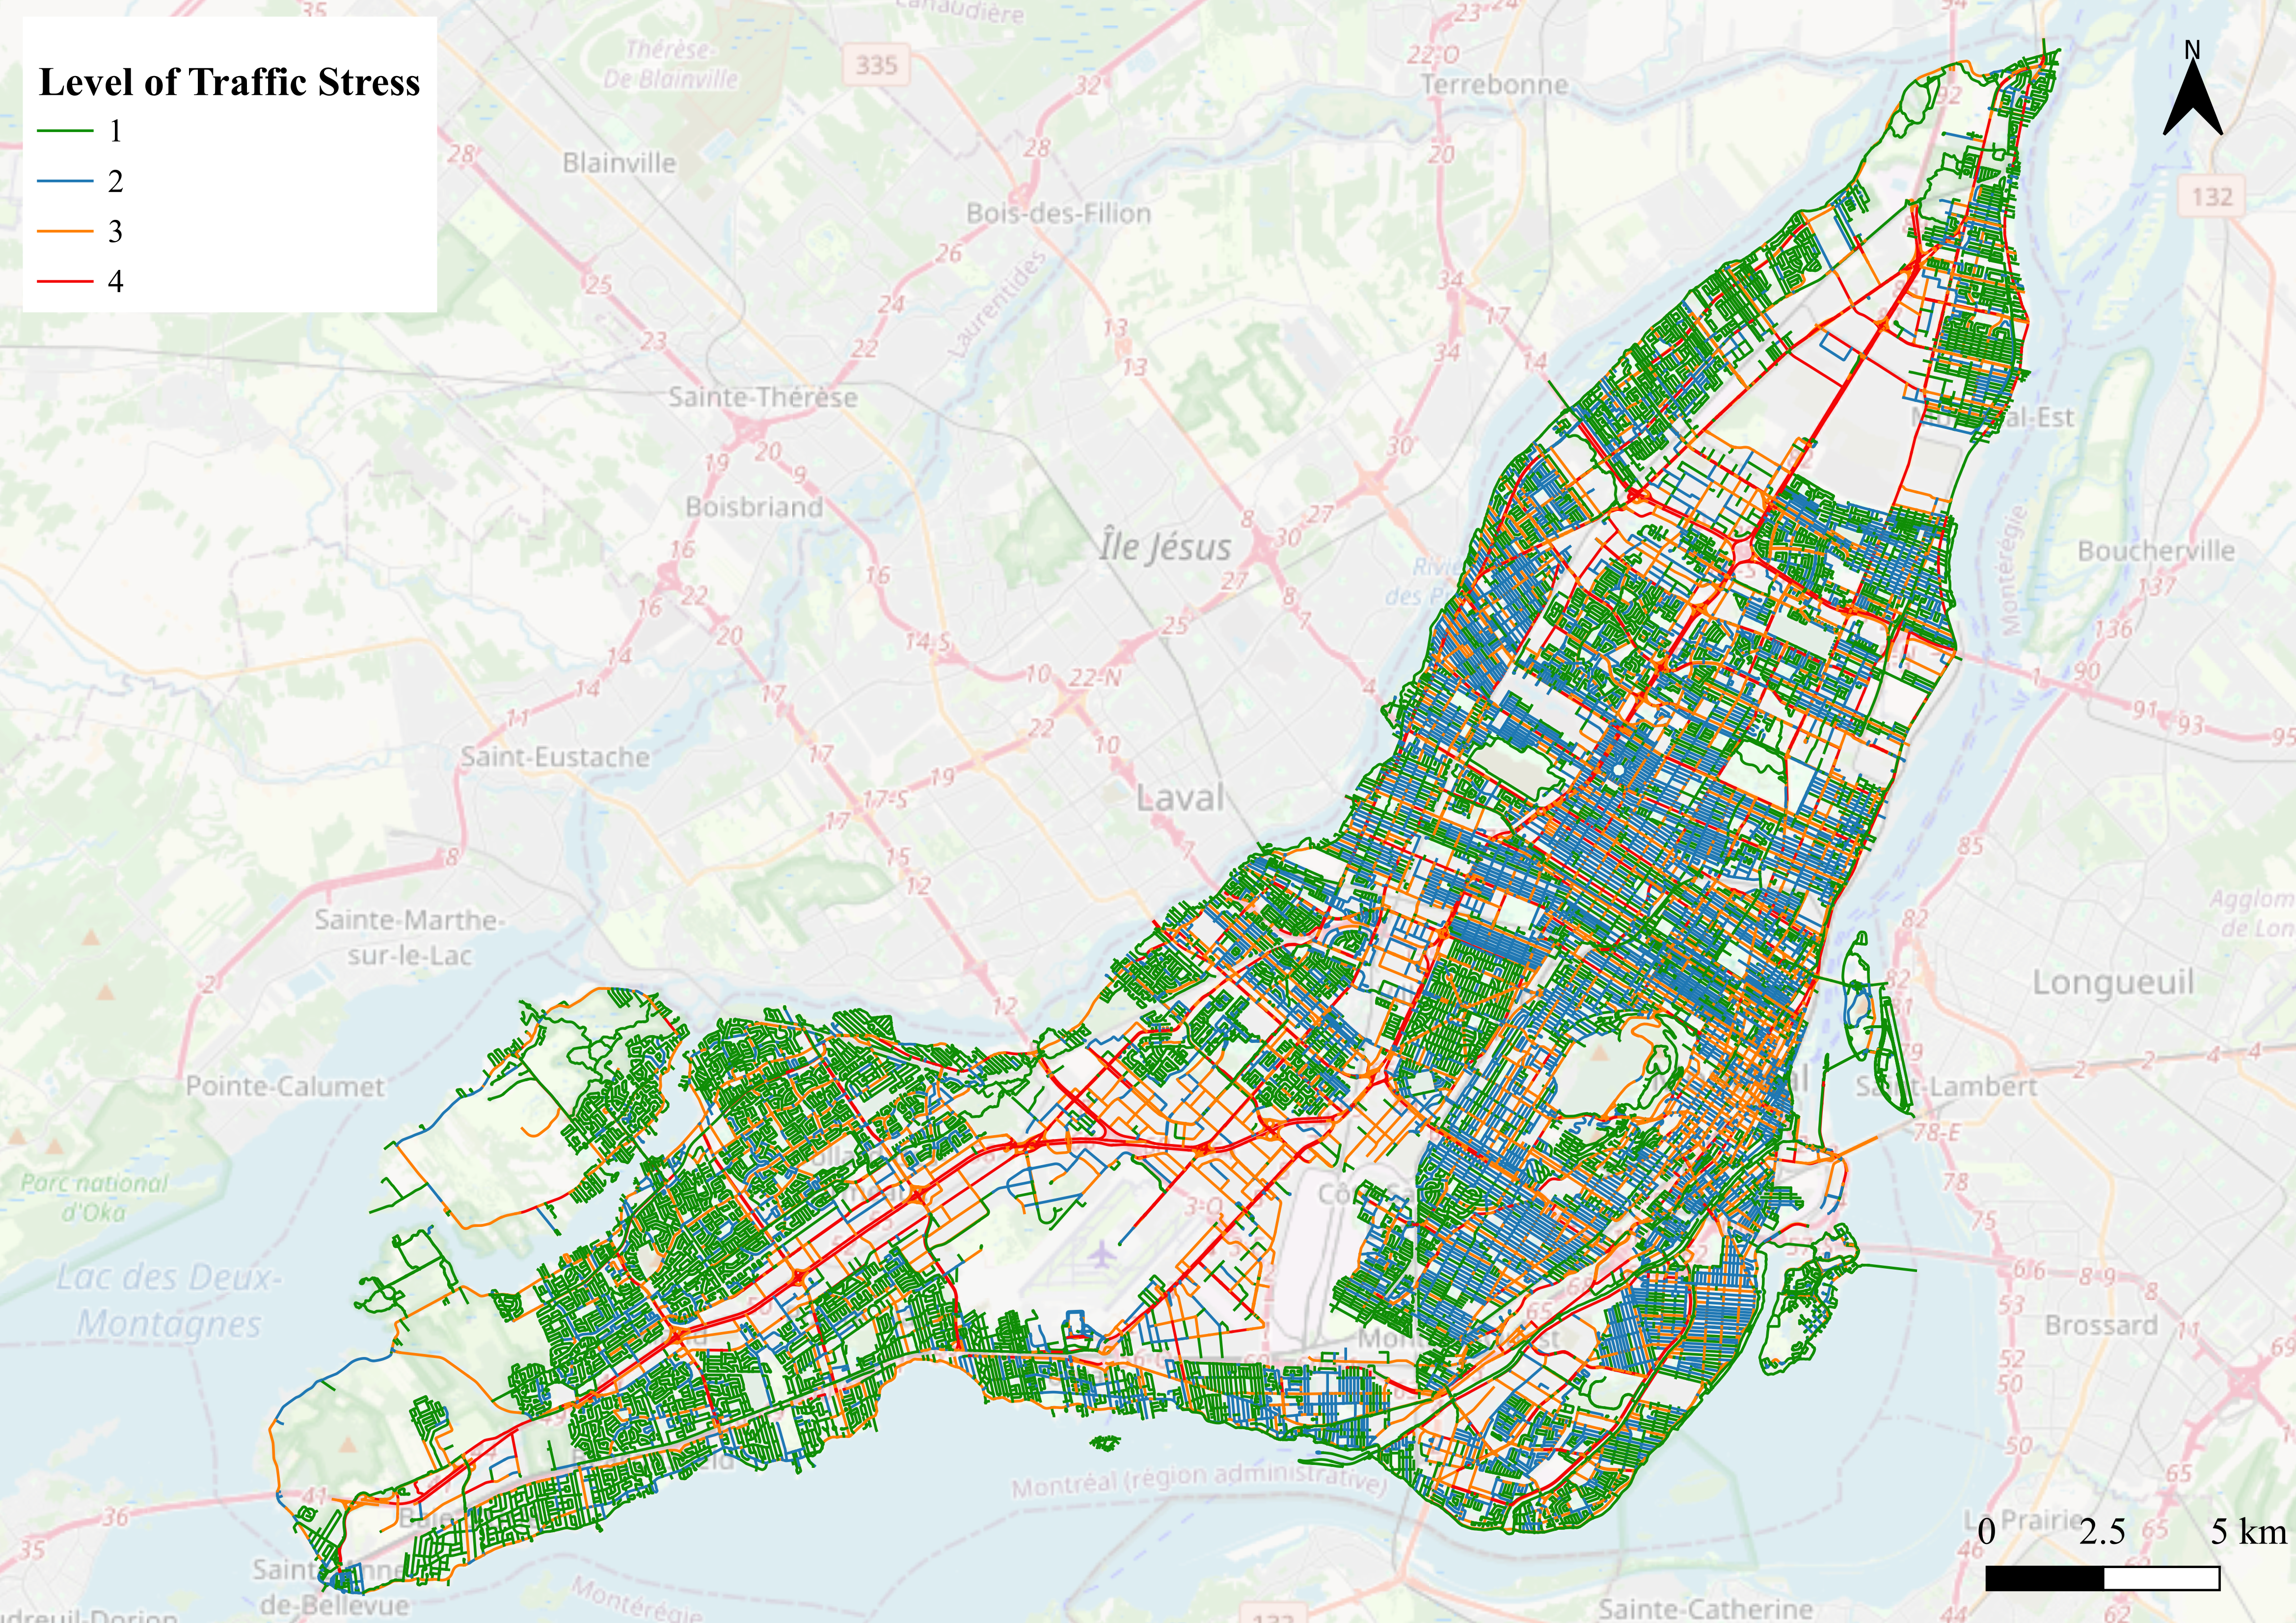
\includegraphics[width=0.7\textwidth]{Figures/LTS_Mapping2.png}
    \caption{Spatial distribution of LTS levels across Montreal's street network.}
    \label{fig:lts_mapping}
\end{figure}

Low-stress facilities (LTS 1--2) are more prevalent in central neighborhoods where cycling infrastructure is relatively dense and well-connected. However, many arterial corridors and major intersections remain classified as high-stress (LTS 3--4), and these high-stress segments often function as network bottlenecks. Even when local low-stress facilities exist, high-stress bottlenecks can dramatically reduce end-to-end network usability by forcing users to traverse uncomfortable or potentially unsafe conditions. This topology has important implications for station placement: locating a station to require access via high-stress links makes it less attractive regardless of its accessibility to local demand concentrations.

In the optimization model, LTS serves two complementary roles. First, it characterizes the comfort and perceived safety of the cycling network. Second, it guides investment decisions by identifying priority corridors for infrastructure improvement. When the algorithm selects a link for upgrade, it is assumed to improve that link to a low-stress standard (LTS 1), with costs specified as a function of the link's initial category. This framework ensures that optimization solutions account for both the current state of the network and the feasible improvements that can be made within budget constraints.

\subsection{Optimization Parameters and Algorithm Settings}\label{subsec:parameters}

The optimization model requires specification of both planning parameters (costs, service requirements) and algorithmic hyperparameters (population size, convergence settings). First, the planning parameters are specified in Table \ref{tab:global_parameters}.

\begin{table}[htbp]
  \caption{Economic and service parameters applied in the station and network optimization model.}
  \label{tab:global_parameters}
  \centering
  \small
  \setlength{\tabcolsep}{6pt}
  \renewcommand{\arraystretch}{1.15}
  \begin{tabularx}{0.85\textwidth}{@{} l X @{}}
    \hline
    \textbf{Parameter} & \textbf{Value} \\\hline
    Dock (capacity-unit) cost, $C_i^{\text{dock}}$ & 500 [CAD\$/unit] \\
    Minimum total demand covered, $D_{\min}$ & 150,000 [trips] \\
    Minimum number of stations, $S_{\min}$ & 30 [stations] \\
    Minimum number of links, $M_{\min}$ & 50 [links] \\
    Link upgrade cost, $C_{ij}^{\text{up}}$ & $\{0; 5{,}000; 10{,}000; 50{,}000\}$ [CAD\$] \\
    & for $\text{LTS}_{ij}=\{1,2,3,4\}$ \\
    \hline
  \end{tabularx}
\end{table}

Cost inputs follow values reported in prior planning studies and system evaluations. Dock costs reflect typical capital expenditures for bike-sharing capacity, while link upgrade costs vary by LTS category, with low-stress facility upgrades commanding higher investment than basic improvements. Links initially classified as LTS 1 require no upgrade and incur zero cost. Minimum service requirements (demand coverage, station count, link count) are specified to prevent degenerate solutions that would be unsuitable for practical planning. Demand and capacity parameters are derived directly from the processed BIXI origin-destination dataset.

Further, Table~\ref{tab:nsga2_hyperparams} presents the baseline NSGA-II settings applied throughout the computational experiments. 

\begin{table}[htbp]
  \centering
  \caption{NSGA-II hyperparameters.}
  \label{tab:nsga2_hyperparams}
  \small
  \renewcommand{\arraystretch}{1.15}
  \begin{tabular}{l @{\hspace{2.0cm}} r}
    \hline
    \textbf{Algorithm Parameter} & \textbf{Value} \\
    \hline
    Crossover probability & 0.90 \\
    Mutation probability & 0.20 \\
    Tournament size & 2 \\
    Initial population size & 3,000 \\
    Number of objectives & 3 \\
    Number of generations & 100 \\
    \hline
  \end{tabular}
\end{table}

These hyperparameters were held constant across all scenarios to ensure that resulting Pareto fronts are directly comparable and that differences in optimization outcomes reflect differences in planning objectives and constraints rather than variations in algorithm configuration.


% -------------------- Results --------------------
\section{Results and Discussion}\label{results}

This section presents results obtained by applying the proposed tri-objective model to the Montreal case study. Because the problem involves competing goals, maximizing demand coverage (Z1), minimizing cyclist stress exposure (Z2), and minimizing investment cost (Z3), the solutions are analyzed in terms of Pareto efficiency. First, the geometry of the approximated Pareto set in objective space is examined, and then planning implications through representative designs mapped onto the study area are interpreted. Finally, the model's robustness is evaluated by re-running the search with alternative constraint thresholds and assessing how the attainable trade-off surface shifts as requirements tighten.


\subsection{Pareto Front Approximation}

The NSGA-II algorithm generates an approximation of the Pareto frontier that captures trade-offs among demand coverage (number of trips), cyclist stress exposure (LTS), and investment cost (CAD\$). Figure~\ref{fig:pareto_2d} presents pairwise projections of the final population in objective space.

\begin{figure}[htbp]
  \centering
  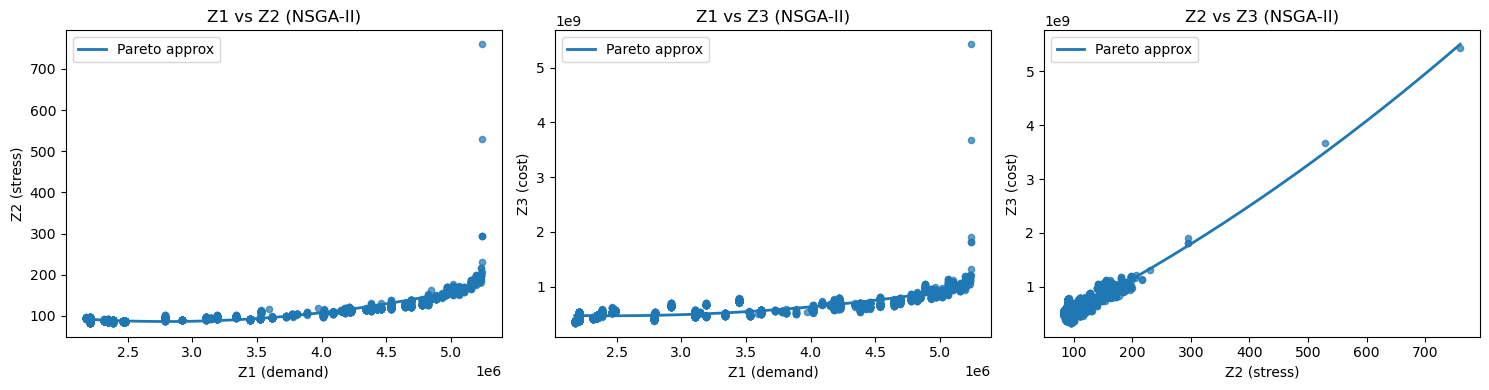
\includegraphics[width=\textwidth]{Figures/Plots_2D_Pop_3000_Gen_100.png}
  \caption{Pairwise projections of the NSGA-II Pareto set showing trade-offs among demand coverage, LTS, and investment cost.}
  \label{fig:pareto_2d}
\end{figure}


The distributions indicate a clear trade-off structure, showing that increasing covered demand typically requires either additional infrastructure upgrades or capacity provisioning, which raises investment costs and may expose more links to higher-stress conditions, reflecting the inherent tension among coverage expansion, comfort, and cost. The $Z_2$–$Z_3$ projection further indicates a strongly increasing, nonlinear relationship, suggesting that reductions in stress are typically achieved through disproportionate increases in upgrade costs. Figure~\ref{fig:pareto_3d} provides the corresponding three-dimensional view of the Pareto set. 

\begin{figure}[htb]
  \centering
  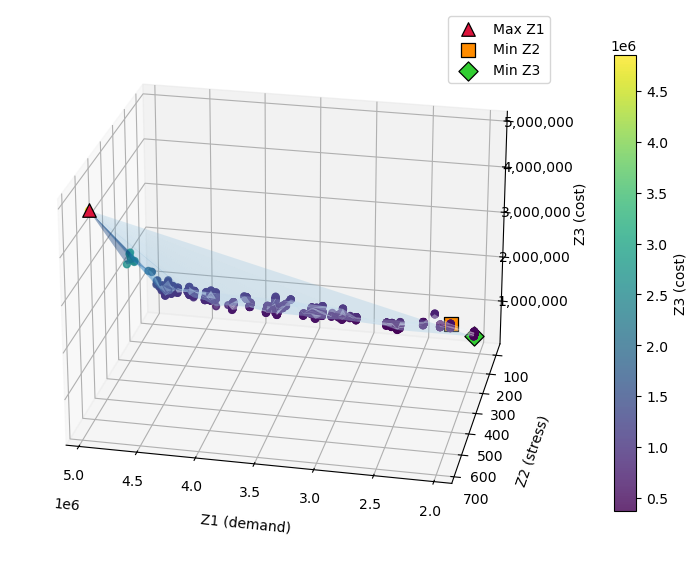
\includegraphics[width=0.65\textwidth]{Figures/Plots_3D_Pop_3000_Gen_100.png}
  \caption{Three-dimensional visualization of the NSGA-II Pareto set in $(Z_1, Z_2, Z_3)$ space, illustrating the structured trade-off surface between coverage, comfort, and cost.}
  \label{fig:pareto_3d}
\end{figure}

The plot shows that non-dominated solutions lie along a structured manifold, revealing a limited number of policy-relevant compromise regions (e.g., moderate coverage with moderate stress and cost versus high-coverage solutions with sharply increased stress and cost). This structure supports the selection of a small set of representative designs for mapping and interpretation in the next section.

\subsection{Analysis of Selected Pareto-Optimal Solutions}

To support interpretation and policy relevance, four representative solutions were extracted and visualized: \textit{Best Demand}, \textit{Best Stress}, \textit{Best Cost}, and a \textit{Balanced solution}. Table \ref{tab:nsga_solutions_size} summarizes the network size of the four representative solutions by reporting the number of selected stations and links in each configuration.

\begin{table}[htbp]
  \caption{Summary of representative NSGA-II solutions and selected network size.}
  \label{tab:nsga_solutions_size}
  \centering
  \small
  \begin{tabular}{@{}lccccc@{}}
    \hline
    \textbf{Solution} & \textbf{Selected Stations} & \textbf{Selected Links} & \textbf{$Z_1$ (million)} & \textbf{$Z_2$ (per link)} & \textbf{$Z_3$ (million)} \\
    \hline
    Best Demand  & 100 & 343 & 4.902 & 1.998 & 48.5 \\
    Best Stress  & 44  & 50  & 2.277 & 1.638 & 5.60 \\
    Best Cost    & 46  & 50  & 2.059 & 1.815 & 3.76 \\
    Balanced     & 93  & 72  & 4.613 & 1.924 & 9.42 \\
    \hline
    \multicolumn{6}{p{0.95\linewidth}}{\footnotesize \textit{Note:} $Z_1$ represents the total number of served trips. $Z_2$ is computed as the average 
    LTS per link, enabling a consistent evaluation of network-wide stress conditions. $Z_3$ denotes the total investment cost in CAD\$.} \\
  \end{tabular}
\end{table}

The \textit{Best Demand} solution activates the largest number of stations (100) and links (343), achieving the highest coverage (4.90 million trips), but at the expense of substantially higher stress and cost. In contrast, the \textit{Best Stress} and \textit{Best Cost} solutions produce much more compact networks, each with around 50 links and fewer than 50 stations, reducing stress and investment but covering only about half of the demand.  The \textit{Balanced solution} provides a more efficient compromise. With 93 stations and 72 links\footnote{The number of selected stations can exceed the number of links because individual links may connect multiple stations located within the service buffers. Because candidate stations are generated within local buffers, several stations can be served by the same upgraded link, resulting in a higher station-to-link ratio.}, it achieves near-maximum demand coverage (4.61 million trips) while reducing both stress and cost relative to the \textit{Best Demand} Scenario. This indicates that most high-demand areas can be effectively served without requiring a fully dense network, provided that key connections are strategically selected. To deepen the analysis, Figure \ref{fig:Map_comparison} compares the corresponding spatial network configurations (selected stations and upgraded links) for these four solutions.

\begin{figure}[htbp]
    \centering
    \begin{subfigure}[b]{0.48\textwidth}
        \centering
        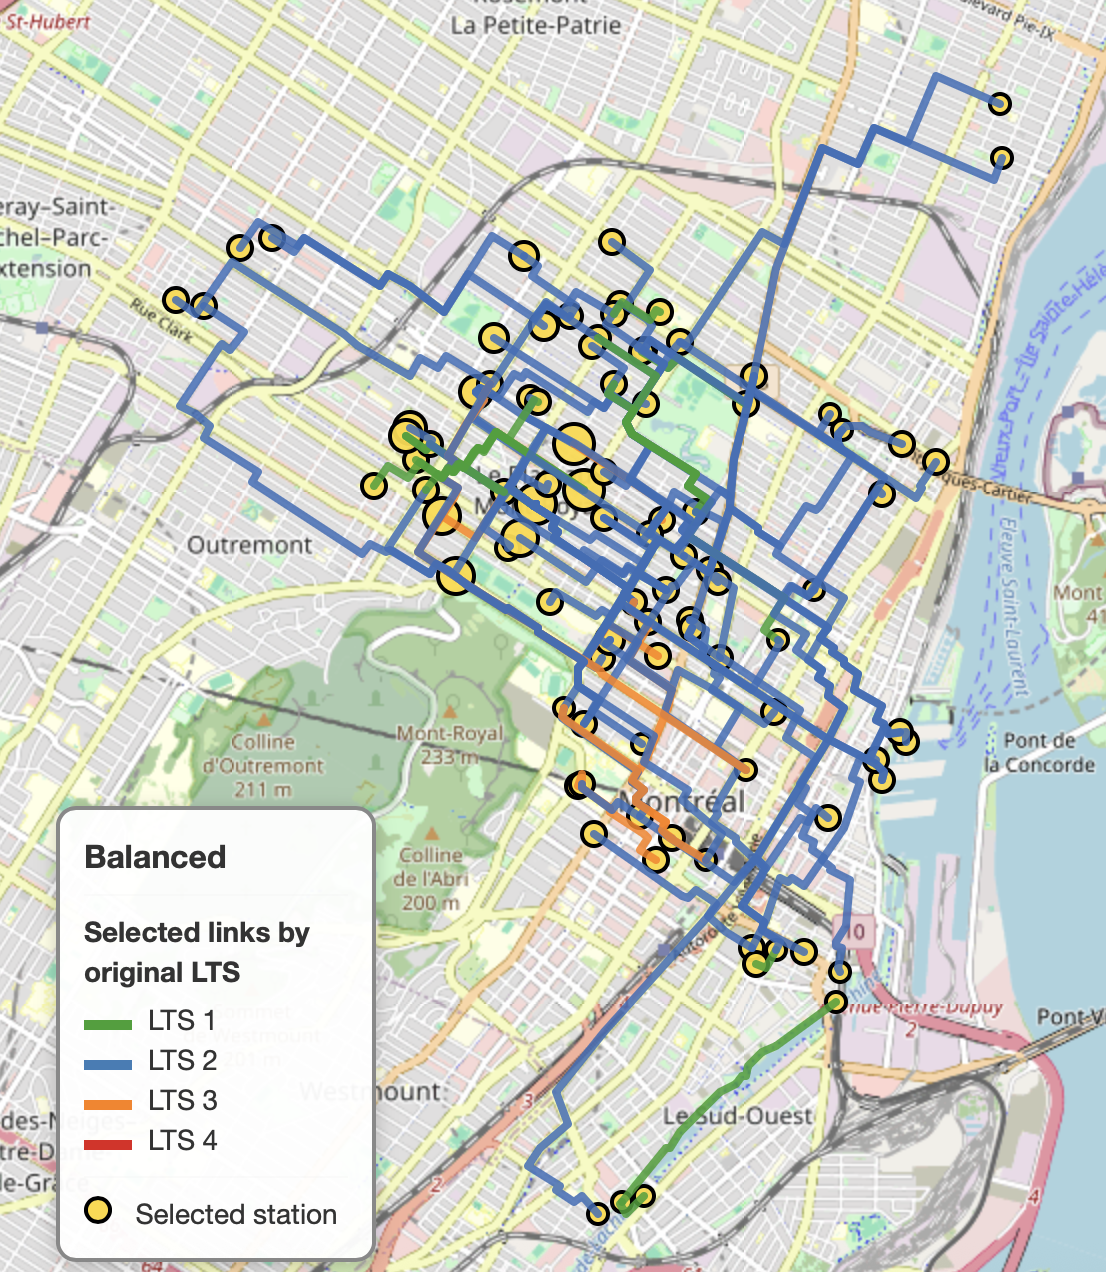
\includegraphics[width=\textwidth]{Figures/nsga_Balanced_Solution_map_3000_100.png}
        \caption{Balanced Solution.}
        \label{fig:Balanced_Solution}
    \end{subfigure}
    \hfill
    \begin{subfigure}[b]{0.48\textwidth}
        \centering
        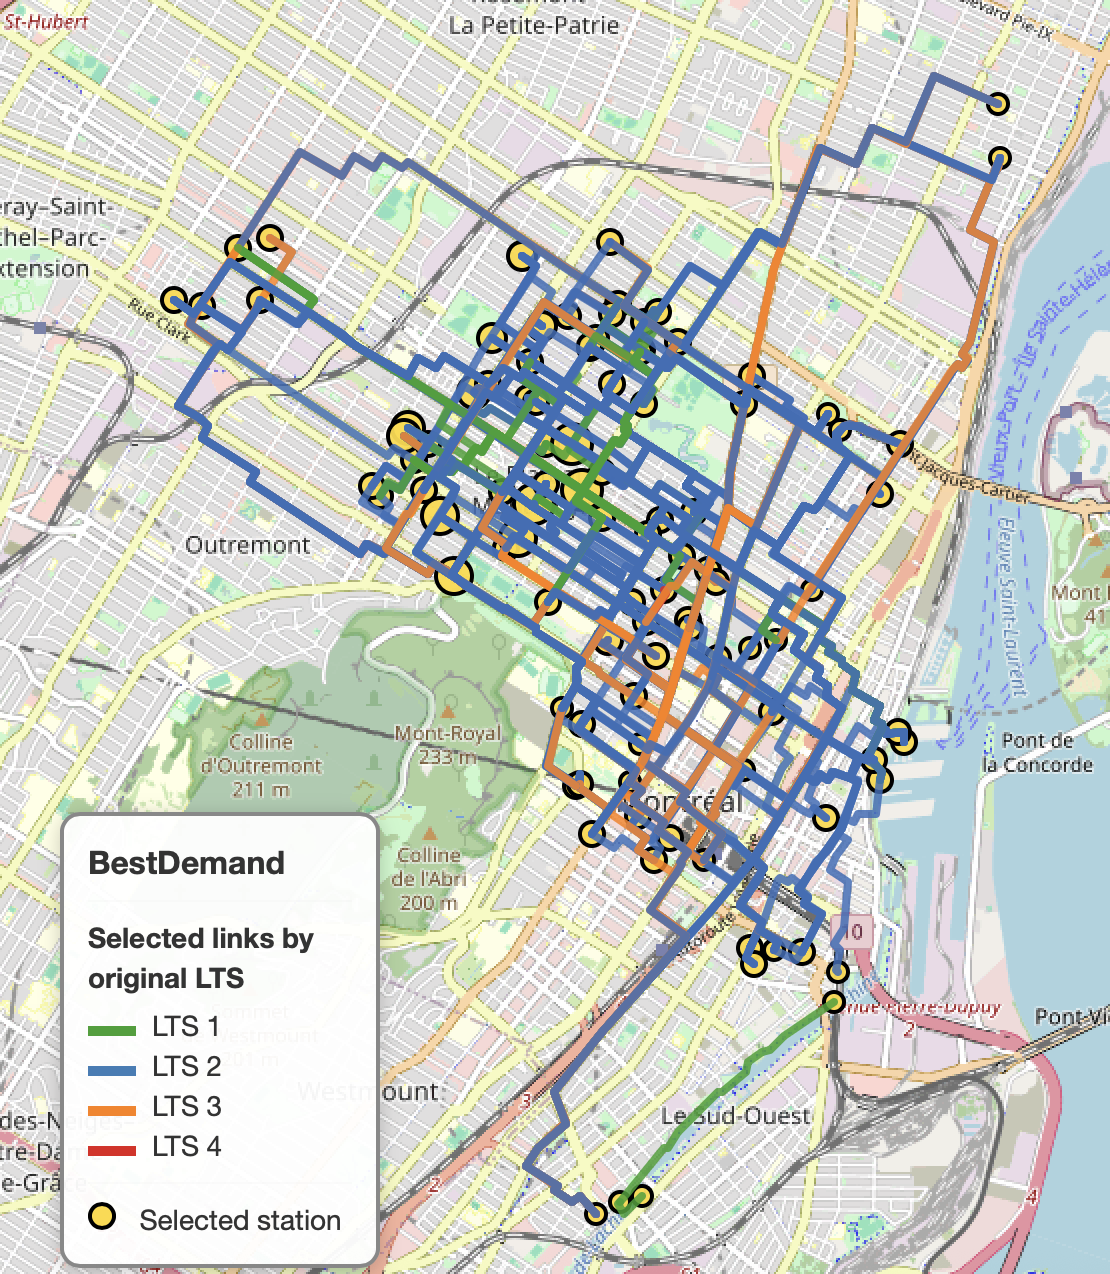
\includegraphics[width=\textwidth]{Figures/nsga_Best_Demand_map_3000_100.png}
        \caption{Best demand solution.}
        \label{fig:Best_Demand}
    \end{subfigure}
    
 \vspace{0.5cm}
    \begin{subfigure}[b]{0.48\textwidth}
        \centering
        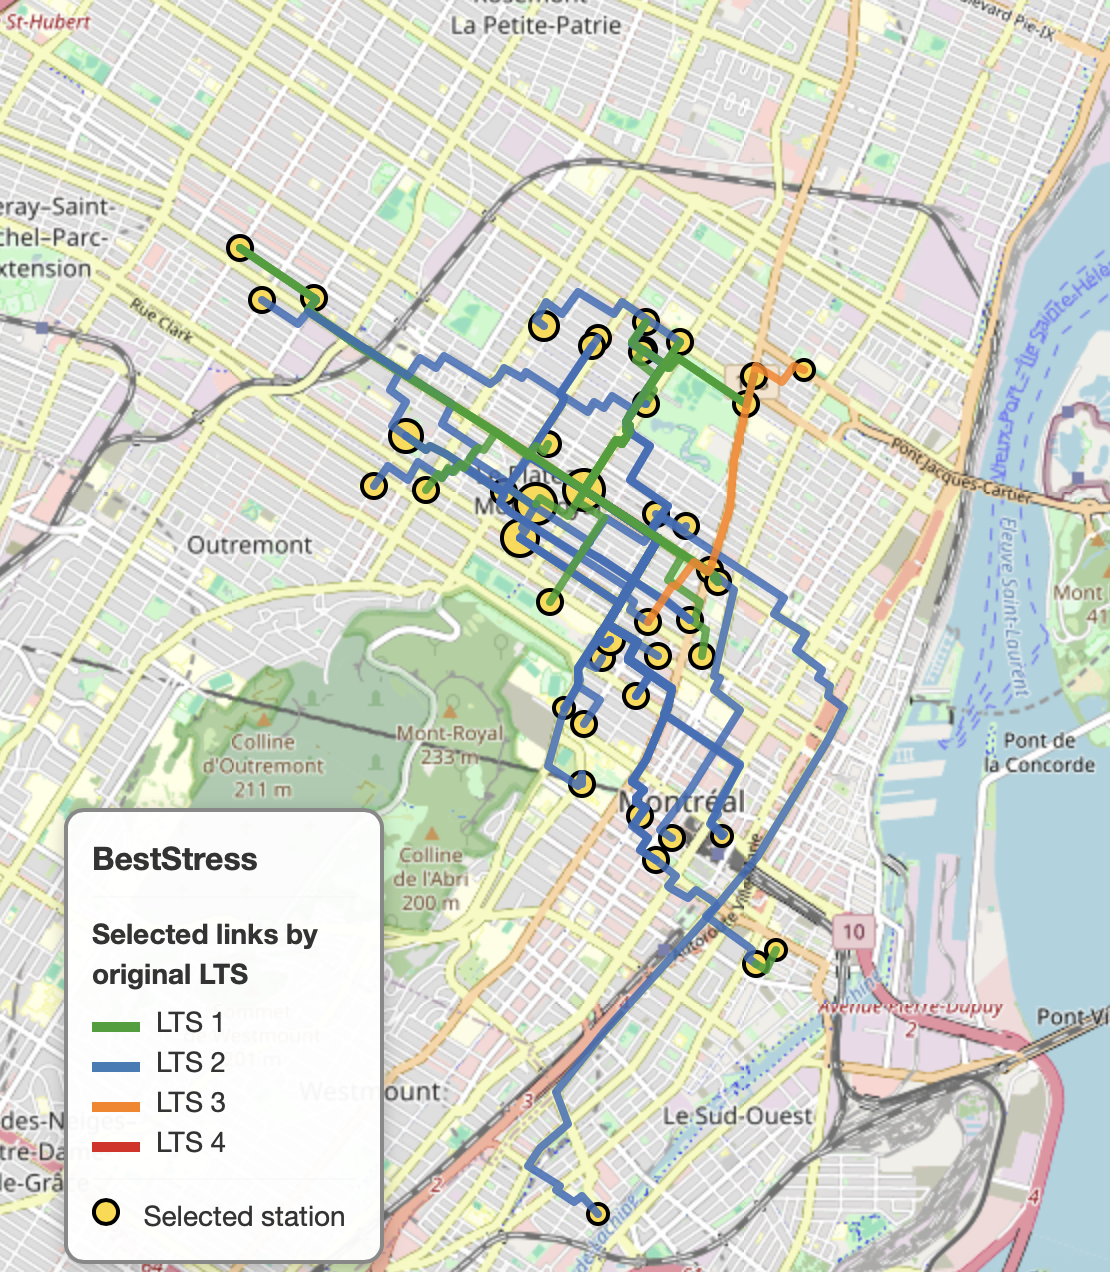
\includegraphics[width=\textwidth]{Figures/nsga_Best_Stress_map_3000_100.png}
        \caption{Best Stress Solution.}
        \label{fig:Best_Stress}
    \end{subfigure}
    \hfill
    \begin{subfigure}[b]{0.48\textwidth}
        \centering
        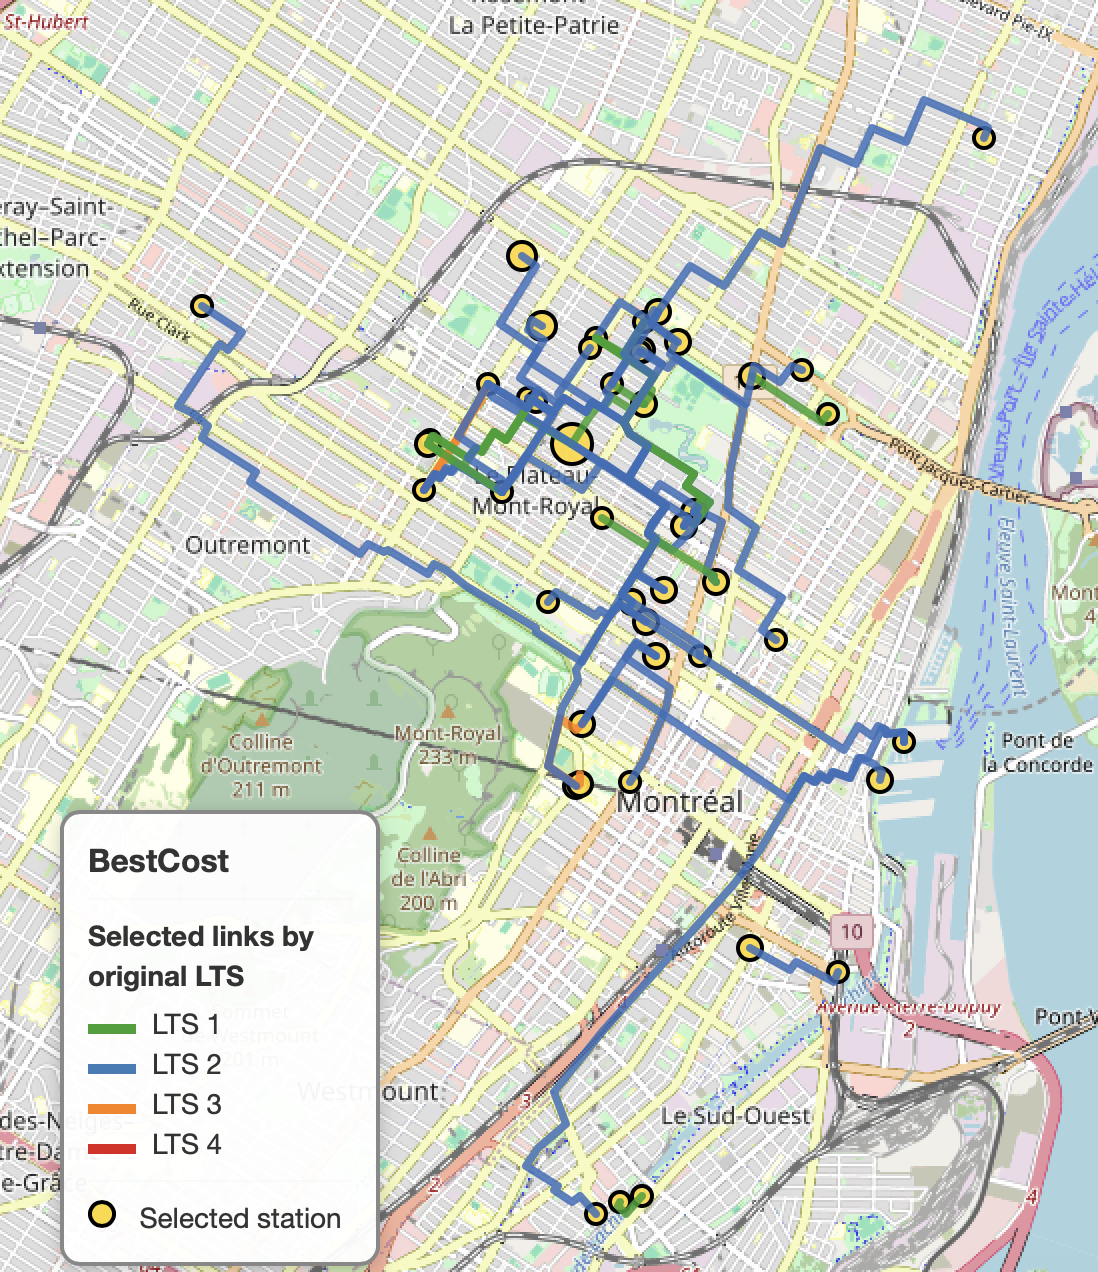
\includegraphics[width=\textwidth]{Figures/nsga_Best_Cost_map_3000_100.png}
        \caption{Best cost solution.}
        \label{fig:Best_Cost}
    \end{subfigure}
    \caption{Network configuration comparison of four representative Pareto-optimal solutions, illustrating distinct planning trade-offs between coverage, comfort, and cost.}
    \label{fig:Map_comparison}
\end{figure}

The network maps highlight clear spatial trade-offs between coverage, comfort, and investment. The \textit{Best Demand} solution concentrates infrastructure along major activity corridors, producing a dense network that maximizes coverage but requires extensive upgrades and higher cost. In contrast, the \textit{Best Stress} solution selectively prioritizes low-LTS corridors, yielding a safer, more coherent network, but with reduced access to some high-demand areas connected via higher-stress links. The \textit{Best Cost} solution adopts a minimal configuration, limiting both station deployment and link upgrades, thereby emphasizing budget efficiency at the expense of spatial coverage. The \textit{Balanced solution} retains the key corridors necessary to serve major demand clusters while avoiding costly and high-stress expansions, achieving a more efficient and policy-relevant compromise, also clustering stations within the service buffer.

\subsection{Modal-Shift and Avoided \texorpdfstring{CO$_2$}{CO2} Potential}\label{subsec:co2_results}

To strengthen the environmental interpretation of the Pareto solutions, the four representative designs are evaluated using the modal-shift and avoided-emissions indicators defined in Section~\ref{subsec:environmental_kpis}. Table~\ref{tab:environmental_kpis} reports an illustrative scenario in which 5\% of served bike-share trips substitute car trips with an average displaced distance of 2.0~km. This conservative scenario is motivated by the literature's caution that bike-share trips can replace a mixture of car, transit, walking, and personal cycling trips rather than only car travel \citep{fuller2013potential, RICCI201528, saltykova2022environmental}. The assumed passenger-vehicle emission factor is 0.2485 kg CO$_2$/km. These values should be interpreted as planning indicators rather than observed emissions reductions, since actual impacts depend on realized ridership, trip lengths, mode substitution, vehicle occupancy, rebalancing operations, and induced demand.

\begin{table}[htbp]
  \caption{Illustrative modal-shift and avoided CO$_2$ indicators for representative Pareto solutions.}
  \label{tab:environmental_kpis}
  \centering
  \small
  \begin{tabular}{@{}lrrrr@{}}
    \hline
    \textbf{Solution} & \textbf{Car-substituting trips} & \textbf{Avoided VKT} & \textbf{Avoided CO$_2$} & \textbf{CO$_2$/cost} \\
    & \textbf{[trips/year]} & \textbf{[km/year]} & \textbf{[t/year]} & \textbf{[t/CAD\$M]} \\
    \hline
    Best Demand & 245,100 & 490,200 & 121.8 & 2.5 \\
    Best Stress & 113,850 & 227,700 & 56.6 & 10.1 \\
    Best Cost & 102,950 & 205,900 & 51.2 & 13.6 \\
    Balanced & 230,650 & 461,300 & 114.6 & 12.2 \\
    \hline
    \multicolumn{5}{p{0.96\linewidth}}{\footnotesize \textit{Note:} Values assume $\rho_c=5\%$, $\bar{d}=2.0$ km, $\omega_c=1$, and $e_c=0.2485$ kg CO$_2$/km. Avoided CO$_2$ values scale linearly with the assumed car-substitution rate and trip distance.} \\
  \end{tabular}
\end{table}

The environmental comparison changes the interpretation of the Pareto set in two ways. First, the \textit{Best Demand} solution produces the largest absolute avoided-emissions potential because it serves the most trips. Under the illustrative assumptions, it avoids approximately 490,200 vehicle-km and 121.8 tonnes of CO$_2$ annually. However, its high infrastructure cost results in only 2.5 tonnes of avoided CO$_2$ per CAD\$ million, making it environmentally inefficient from an investment perspective. Second, the \textit{Balanced solution} captures nearly the same emissions potential as the \textit{Best Demand} solution (114.6 versus 121.8 tonnes CO$_2$ annually) while requiring far lower investment. This yields 12.2 tonnes CO$_2$ avoided per CAD\$ million, nearly five times the cost-effectiveness of the demand-maximizing design. The \textit{Best Cost} solution achieves the highest emissions cost-effectiveness because it is inexpensive, but its absolute avoided-emissions potential is less than half that of the balanced scenario.

These results are relevant for a transport-environment framing because they show that the solution with the greatest ridership is not necessarily the most defensible climate-policy investment. If the objective is to maximize absolute CO$_2$ reductions, demand-oriented expansion may appear attractive. If the objective is to allocate limited public funds efficiently, the balanced and cost-oriented solutions perform better. The balanced scenario is therefore the strongest candidate when environmental performance, cost discipline, and network comfort are considered jointly. This interpretation is consistent with broader active-mobility evidence showing that climate benefits depend on the amount of motorized travel actually displaced \citep{BRAND2021102764, MCQUEEN2020102482}. Importantly, this conclusion depends on the assumption that modal substitution is proportional to served demand. If low-stress infrastructure attracts a higher share of former car users than high-stress infrastructure, then comfort-oriented scenarios may generate additional emissions benefits beyond those captured by the simple proportional model. This reinforces the need for future survey-based calibration of $\rho_c$ by corridor type, user group, and LTS condition.

\subsection{Sensitivity Analysis}

A sensitivity analysis is conducted with respect to the number of stations ($S^{\min}$) and links ($M^{\min}$) to examine how the solution space responds to variable design requirements. For each parameter, the model is re-optimized under different threshold values, allowing comparison of how the Pareto front shifts as constraints become more restrictive. The discussion below focuses on normalized indicators so that changes in coverage, comfort, and cost can be interpreted relative to infrastructure scale rather than absolute network size. Full-value sensitivity tables and Pareto-front projections are reported in \ref{app:sensitivity_details}.

\subsubsection{Station Variation}

To assess how minimum station requirements affect network performance, the model is re-optimized for four values of $S_{\min}\in\{30,40,50,60\}$. 

\begin{table}[!ht]
  \caption{Normalized sensitivity analysis results for different minimum station constraints ($S_{\min}$).}
  \label{tab:sensitivity_smin_normalized}
  \centering
  \small
  \begin{tabular}{@{}lcccc@{}}
    \hline
    \textbf{$S_{\min}$} & \textbf{30} & \textbf{40} & \textbf{50} & \textbf{60} \\
    \hline
    Max Z1 / station & 48,603 & 49,284 & 49,534 & 49,608 \\
    Min Z2 / link    & 1.78   & 1.82   & 1.92   & 1.98   \\
    Min Z3 / (station+link) & 4,065.3 & 4,156.5 & 4,237.1 & 4,338.7 \\
    \hline
  \end{tabular}
\end{table}

The results reveal a clear efficiency trade-off. Demand captured per station increases modestly as the minimum station requirement becomes less restrictive, rising from 48,603 trips per station at $S_{\min}=30$ to 49,608 at $S_{\min}=60$. This pattern suggests that larger station requirements push the optimization toward locations with stronger underlying demand, particularly within the dense downtown activity clusters identified in the case study. In other words, when the model is forced to activate more stations, it still prioritizes high-yield sites. The gain in demand is accompanied by weaker comfort and higher investment intensity. The stress per link increases from 1.78 to 1.98 as $S_{\min}$ rises, indicating that additional stations require the network to rely on links with somewhat less favorable LTS characteristics. At the same time, cost per infrastructure element increases from 4,065.3 to 4,338.7, confirming that each incremental expansion step becomes more expensive once the most efficient station--link combinations have already been selected. Taken together, the sensitivity analysis indicates that increasing the number of stations does not necessarily lead to proportional gains in demand coverage. Instead, additional stations primarily expand spatial reach, often at the expense of higher stress levels and greater infrastructure intensity. Moderate station expansion can therefore be justified when the objective is to improve access and coverage. However, the results also reveal diminishing marginal returns, as increasingly stringent station requirements yield only limited gains in demand while incurring greater comfort and cost penalties.

\subsubsection{Links Variation}

To examine how stronger connectivity requirements affect infrastructure efficiency and comfort, the model is re-optimized for four values of the minimum number of selected links, $M_{\min}\in\{50,100,150,200\}$.

\begin{table}[htbp]
  \caption{Normalized sensitivity analysis results for different minimum link constraints ($M_{\min}$).}
  \label{tab:sensitivity_mmin_normalized}
  \centering
  \small
  \begin{tabular}{@{}lcccc@{}}
    \hline
    \textbf{$M_{\min}$} & \textbf{50} & \textbf{100} & \textbf{150} & \textbf{200} \\
    \hline
    Max Z1 / station & 49,008 & 49,045 & 49,190 & 49,597 \\
    Min Z2 / link    & 1.74   & 1.65   & 1.58   & 1.58  \\
    Min Z3 / (station+link) & 4,562.5 & 5,311.9 & 5,971.2 & 6,273.2 \\
    \hline
  \end{tabular}
\end{table}

The results point to a different mechanism. Demand captured per station remains nearly unchanged across scenarios, varying only from 49,008 to 49,597 trips. This stability indicates that increasing the minimum number of links does not materially improve the productivity of each station. Instead, the constraint mainly changes the amount of supporting infrastructure required around a broadly similar set of demand-serving locations. At the same time, the stress per link declines from 1.74 at $M_{\min}=50$ to 1.58 at $M_{\min}=150$, after which it stabilizes. These results indicate that, as minimum link requirements increase, the optimization can still construct relatively low-stress corridors on a per-link basis, preserving infrastructure quality. However, this comes at a substantial cost, as the per-element cost rises sharply from 4,562.5 to 6,273.2. This reflects the increasing difficulty of maintaining low-stress connectivity as the network expands, requiring more expensive upgrades. Consequently, the sensitivity analysis shows that increasing link minimums does not meaningfully enhance demand coverage, but it does reduce network stress at a significant financial premium. Link expansion should therefore be interpreted primarily as a connectivity- and quality-driven intervention, rather than as a mechanism to increase demand, and should be applied only when the planning context justifies the additional investment.

% -------------------- Policy Implications --------------------

\section{Discussion and Policy Implications}
\label{policy}

This section translates the optimization results into actionable insights for policy and planning. It synthesizes key findings and identifies how infrastructure decisions can be structured to balance demand coverage, comfort, and cost in practical implementation contexts. The discussion also considers how Velora can be used as a recurring decision-support platform, rather than as a single case-study model, for scenario testing and stakeholder communication.

\subsection{Key Findings and Policy Relevance}

The optimization results and sensitivity analyses reveal four central findings with direct implications for bike-share network planning: (i) First, concentrated investment in high-demand areas with low-stress infrastructure generates substantially higher returns than distributed expansion. The Pareto-optimal solutions cluster around central Montreal neighborhoods with existing low-stress facilities, yielding 4.5--4.9 million trips at costs of 5.24--30.6 million dollars. Sensitivity analysis shows that expanding beyond these core areas yields diminishing returns: adding stations beyond 50 increases coverage by only 2.3\% while raising costs by 46\%. Similarly, extending links beyond 150 increases costs by 184\%, with negligible gains in demand. This pattern suggests that early-stage bike-share development should concentrate resources on high-demand, infrastructure-feasible zones before pursuing system-wide expansion; (ii) Second, the sensitivity analysis indicates that station and link constraints influence the system in distinct ways. Enhancing the number of stations predominantly broadens coverage, with marginal improvements in demand efficiency, but also increases stress levels and infrastructure costs due to dependence on less-optimal links. Conversely, increasing the number of links results in denser connectivity and reduced stress, while necessitating higher investment without significant additional demand benefits. Station expansion primarily aims to improve coverage, balancing comfort and cost, whereas link expansion affects network connectivity and service quality. Consequently, station policies should prioritize accessibility, whereas link policies should be employed selectively to optimize connectivity and system resilience; (iii) Third, the optimization framework demonstrates that substantial demand can be served via low-stress infrastructure. Solutions that achieve 90\% peak-demand coverage maintain mean link stress levels comparable to or better than the network median. This indicates that comfort is not inherently incompatible with coverage or cost efficiency. Treatment of stress as a binding service standard (rather than a residual outcome) is therefore both feasible and justified, particularly given evidence that low-stress access expands the population willing to use bike-share systems beyond core cycling demographics; and (iv) Fourth, the environmental KPI layer shows that climate benefits should be evaluated using both absolute avoided emissions and cost-effectiveness. The demand-maximizing solution produces the largest avoided-CO$_2$ potential, but the balanced solution delivers nearly the same emissions benefit at far lower cost, making it more attractive for climate-oriented infrastructure budgeting.

\subsection{Planning Implications}

\subsubsection{Network Development Sequencing}

The results suggest a staged planning approach aligned with the natural structure of optimal solutions. First, planners should define the target station footprint in terms of explicit coverage and equity objectives. The sensitivity analysis indicates that station minima in the range 40--50 represent an efficiency frontier: beyond 60 stations, cost and stress penalties escalate sharply relative to coverage gains. Second, once the station footprint is fixed, the minimum set of links required to connect those stations via low-stress corridors should be identified. This framing (better connectivity rather than higher link density) is critical because the sensitivity analysis indicates that link constraints primarily affect infrastructure intensity rather than demand efficiency. Third, station and link investments should be bundled as coordinated corridor packages rather than dispersed separately. This ensures immediate value realization and avoids fragmentation, in which stations lack low-stress access or bikeway upgrades lack nearby stations. Fourth, implementation should be phased by demand and infrastructure feasibility, deploying high-demand, feasible-connectivity zones before secondary demand areas. Only after the core network has matured should further expansion be committed.

\subsubsection{Setting Infrastructure Thresholds}

The sensitivity analysis highlights the importance of defining infrastructure thresholds \textit{a priori}, rather than allowing them to emerge implicitly from unconstrained expansion. Minimum requirements for stations and links act as structural parameters that shape the feasible design space and strongly influence the resulting trade-offs between coverage, comfort, and cost. These thresholds should therefore be calibrated deliberately to reflect planning priorities. Station thresholds should be aligned with access and equity objectives to ensure sufficient spatial coverage without forcing inefficient expansion into lower-demand or higher-stress areas. Beyond a certain level, increasing the number of stations yields diminishing returns, as additional coverage comes at the expense of higher infrastructure intensity and reduced network quality. Link thresholds, in contrast, primarily govern connectivity and network structure. While additional links can improve local continuity and reduce stress, they also impose high costs when imposed excessively. Link requirements should therefore remain modest and purpose-driven, applied only where improved connectivity or resilience is essential.

\subsubsection{Comfort as a Service Standard}

The integration of stress as an explicit optimization objective demonstrates that low-stress access is achievable within cost and coverage constraints. Formalization of comfort targets (for example, ensuring that 80\% of trips are accessible via LTS 1--2 facilities) should accompany coverage targets. This is particularly important for expanding bike-share use beyond core cycling populations. Operationally, this requires: (i) establishing quantified comfort thresholds in network plans, (ii) including comfort objectives in project evaluation, and (iii) rejecting station deployments that cannot be served by low-stress access without severe system-wide comfort degradation. In Montreal's case, the relative abundance of low-stress infrastructure in central areas allows this standard to be met in core networks; aggressive expansion into arterial-dominated peripheral areas would violate comfort standards and should be avoided or accompanied by substantial bikeway investment.

\subsubsection{Environmental Appraisal as a Planning Standard}

For a transport-environment decision process, coverage and comfort metrics should be paired with explicit modal-shift and emissions KPIs. The results show why: two scenarios can serve similar numbers of trips but differ sharply in infrastructure cost, stress exposure, and emissions cost-effectiveness. Agencies should therefore report avoided VKT, avoided CO$_2$, and tonnes CO$_2$ avoided per CAD\$ million alongside conventional indicators such as station count and network length. Because the avoided-emissions estimates depend on the share of bike-share trips that replace car travel, and because bike-share mode substitution can include transit and active modes \citep{fuller2013potential, saltykova2022environmental}, policy reports should present sensitivity ranges rather than a single deterministic value. In practice, this means evaluating each recommended infrastructure package under low, medium, and high car-substitution assumptions and updating those assumptions through user surveys, intercept interviews, and observed travel-behavior data after implementation. Embedding this KPI layer in Velora allows cities to treat cycling investments as climate-policy instruments while remaining transparent about uncertainty.

\subsubsection{Platform-Based Scenario Governance}

Velora extends these planning implications by making assumptions and trade-offs visible during the decision process. Instead of presenting stakeholders with a single recommended network, the platform allows agencies to compare best-demand, best-stress, best-cost, and balanced scenarios under consistent metrics. This supports a more transparent governance process in which elected officials, technical staff, operators, and community representatives can see how changing a threshold or unit cost affects the resulting station footprint, link upgrades, budget requirement, and environmental KPI profile. The saved-run structure also creates an audit trail: each scenario is associated with its data inputs, configuration parameters, objective values, and spatial outputs. This is valuable for policy-making because infrastructure decisions often evolve over multiple rounds of consultation, budget revision, and engineering review. Decision-support research in cycling planning emphasizes this role of interactive scenario analysis for more informed infrastructure prioritization \citep{silvestriCyclabilityDSS2024}. A platform workflow allows each revision to be documented and compared rather than treated as an isolated analysis.

In practical implementation, Velora can support four policy tasks. First, it can be used for budget negotiation by showing the marginal benefits of additional stations or links. Second, it can support corridor packaging by identifying groups of stations and link upgrades that should be delivered together to avoid fragmented investment. Third, it can be used for climate appraisal by translating served demand into avoided VKT, avoided CO$_2$, and emissions cost-effectiveness under transparent substitution assumptions. Fourth, it can be used for monitoring and adaptive planning by re-optimizing after new demand data, new bikeway projects, revised cost assumptions, or observed modal-shift evidence become available. In this sense, Velora functions as a planning laboratory for cycling investment decisions: it does not replace professional judgment, engineering design, or public consultation, but it provides a quantitative structure through which those judgments can be compared.

\subsection{Broader Policy Framework}

The findings support a reorientation of bike-share policy from growth maximization (emphasizing station count, link miles, or nominal ridership) toward value maximization (emphasizing cost-per-trip-served, comfort-adjusted coverage, and financial sustainability). Specifically, this implies:

\begin{enumerate}
    \item Evaluating projects by cost-per-trip metrics rather than network size
    \item Treating comfort as a binding standard rather than a secondary consideration
    \item Using optimization tools to make infrastructure trade-offs explicit in stakeholder engagement
    \item Reporting avoided VKT, avoided CO$_2$, and emissions cost-effectiveness under clearly stated modal-shift assumptions
    \item Phasing implementation with built-in flexibility to adapt based on realized demand patterns and observed environmental performance.
\end{enumerate}

These principles have broader applicability across cities with varying demand distributions and infrastructure endowments. The methodology employed here (multi-objective optimization with explicit comfort constraints implemented through Velora) is transferable to other contexts. However, specific parameter choices (station counts, link thresholds, comfort targets) must be calibrated to local demand concentrations, existing infrastructure, and policy objectives. In cities with more dispersed demand patterns than Montreal, higher station and link minima may be justified; in cities with more constrained budgets or existing extensive bikeway networks, lower minima may be appropriate. The key contribution is a platform that makes these trade-offs visible and quantifiable rather than implicit or intuition-based. For Montreal specifically, these findings suggest pursuing a disciplined growth strategy: establish a core network of 45--55 stations and 90--110 links in the high-demand central zone, formalize 85 \%-plus comfort coverage as a service standard, phase implementation over 3--5 years prioritizing high-demand corridors with existing low-stress infrastructure, and reserve expansion decisions for later phases based on demonstrated demand and explicit cost-benefit thresholds. Periodic re-optimization in Velora as demand patterns and infrastructure change allows the system to adapt without being locked into outdated designs. The broader implication is that bike-share network design is not primarily a question of how much infrastructure to build, but rather how to allocate limited infrastructure strategically across competing objectives. Platform-based optimization makes this allocation process transparent and defensible, supporting more robust and sustainable infrastructure investment decisions.

% -------------------- Conclusions --------------------

\section{Conclusion}\label{conclusion}

This paper addresses a long-standing gap in bike-share planning: the separation between bikeway infrastructure and station-based system design. By developing Velora, a multi-objective decision-support platform that jointly optimizes station locations, link selection, and capacity allocation, the work enables planners to navigate explicit trade-offs among demand coverage, cyclist comfort, procurement costs, and environmental performance within a unified and repeatable workflow. The methodological contribution centers on formulating a tri-objective MILP, solving it via NSGA-II, embedding the optimization process in a platform that supports data validation, scenario configuration, interactive mapping, saved runs, and comparison of representative alternatives, and adding a modal-shift KPI layer that estimates avoided VKT and CO$_2$ potential. This approach differs from prior work in four ways: first, it treats bikeway quality and station placement as co-dependent decisions rather than as sequential planning steps; second, it reveals the Pareto structure of the planning problem, thereby identifying which combinations of coverage, comfort, and cost are achievable within budget constraints; third, it makes the optimization process accessible as a decision-support application rather than only as an offline analytical exercise; and fourth, it connects bicycle infrastructure planning to transport-environment appraisal through explicit avoided-emissions indicators.

When applied to Montreal using 2025 BIXI trip data, the framework yields a Pareto set characterized by clear trade-off structures. A balanced solution with 93 stations and 72 links serves 4.6 million trips at CAD\$ 9.42 million, with moderate stress exposure, capturing 94\% of achievable demand while avoiding the doubling of cost and the five-fold increase in stress incurred by demand-maximizing designs. Under an illustrative modal-shift scenario in which 5\% of served bike-share trips replace 2.0-km car trips, the balanced solution avoids approximately 461,300 vehicle-km and 115 tonnes of tailpipe CO$_2$ annually, while delivering almost the same avoided-emissions potential as the demand-maximizing solution at far lower cost. This result demonstrates that most high-demand areas can be effectively served by selectively placing infrastructure rather than by full network densification. Sensitivity analyses reveal clear asymmetries between station and link expansion as policy levers. Increasing station requirements primarily expands spatial coverage, with only marginal gains in demand efficiency, but at the expense of higher stress levels and greater infrastructure intensity. In contrast, increasing link requirements does not improve demand efficiency and instead enforces denser connectivity, which can maintain relatively low-stress links but at a substantially higher cost. These patterns indicate that stations function primarily as access and coverage instruments, whereas links primarily govern network structure and stress intensity. Planning should therefore treat them as distinct levers: moderately calibrated station minima balance coverage with cost, while link minima should be reserved for specific topological, resilience, or emissions-mitigation objectives. 

Further, some limitations and directions for future work should be acknowledged. The study focuses on a Montreal subregion and assumes static, aggregated demand, omitting temporal dynamics such as peak variation and strong seasonality. Rider heterogeneity is not explicitly modeled, and the use of LTS as a proxy for comfort does not fully capture subjective safety perceptions or the complexity of intersections. From a modeling perspective, the framework relies on deterministic inputs for demand, costs, and infrastructure effects, which may evolve over time. Operational aspects of bike-sharing systems, such as rebalancing, vehicle availability, and station congestion, are not considered. Behavioral feedback effects, including induced demand from improved infrastructure, are also not represented. The environmental analysis is intentionally presented as potential rather than observed impact: modal substitution rates, trip distances, vehicle occupancy, transit substitution, bike-share operations, rebalancing, and life-cycle infrastructure emissions can all change net CO$_2$ benefits \citep{RICCI201528, saltykova2022environmental}. From a platform perspective, Velora currently focuses on strategic planning and scenario comparison; future versions should incorporate role-specific permissions, more detailed reporting functions, uncertainty visualization, and direct integration with municipal GIS asset-management systems. Finally, transferability is limited because Montreal's dense core and existing cycling infrastructure may not generalize to other urban contexts. In this context, future work should incorporate time-varying demand, uncertainty, behavioral and modal-shift modeling, life-cycle emissions accounting, extend the analysis to the citywide scale, integrate multimodal connections, and evaluate the platform with practitioners through structured usability and decision-making studies.

In conclusion, the main contribution of this study is to demonstrate that explicit, quantifiable trade-off analysis can be operationalized as a practical decision-support platform for disciplined infrastructure allocation and environmental policy appraisal. Rather than asking ``how much to build,'' planning becomes ``how to allocate strategically, under which assumptions, and with what mobility, comfort, cost, and emissions consequences.'' For cities with demand patterns similar to Montreal, Velora provides a practical basis for moving beyond \textit{ad hoc} expansion toward evidence-based network design that simultaneously balances coverage, comfort, cost, and climate-mitigation potential. Platform-based optimization makes these trade-offs transparent, reproducible, and defensible, supporting more sustainable and equitable infrastructure investment decisions.

\appendix
\setcounter{figure}{0}
\setcounter{table}{0}
\renewcommand{\thefigure}{\thesection.\arabic{figure}}
\renewcommand{\thetable}{\thesection.\arabic{table}}
\renewcommand{\theequation}{\thesection.\arabic{equation}}

\section{Velora Platform Supplementary Material}\label{app:velora_platform}

This appendix provides additional details on Velora's functioning, software modules, user workflow, and representative interface outputs. Velora was implemented as a web-based decision-support platform that connects a Streamlit user interface with a persistent analytical back-end. The purpose of the platform is to make the optimization model usable in repeated planning contexts, where users need to test assumptions, compare alternatives, and reopen saved runs.

\subsection{Platform Functioning}

Velora follows a scenario-based workflow. A user begins by uploading a station table and a geospatial cycling network. The station table contains station names, coordinates, observed trip volumes, and optional dock estimates. The network layer contains link geometries and LTS values, with link length used directly when available or computed from geometry otherwise. The platform then validates the inputs, standardizes field names, removes incomplete records, and converts spatial layers into a projected coordinate reference system suitable for distance and buffer operations.

After data preparation, Velora creates candidate station alternatives around each existing or proposed station. These candidates allow the optimization engine to test whether small local relocations improve connectivity to low-stress links while maintaining access to the same demand market. The platform then clips the network to the relevant study area, constructs candidate links between station alternatives, estimates link-level stress and cost attributes, and runs the NSGA-II optimization procedure. Completed runs are stored with their configuration, objective values, station selections, link selections, Pareto rows, map-ready files, and automatically generated report material. This report-generation function is intended to reduce the distance between technical optimization outputs and the documents typically needed for municipal decision-making, including city reports, investment summaries, and stakeholder-facing scenario briefs.

Figure~\ref{fig:velora_control_center} shows the Velora control center, which frames the workflow around data preparation, scenario exploration, and city-report generation.

\begin{figure}[htbp]
  \centering
  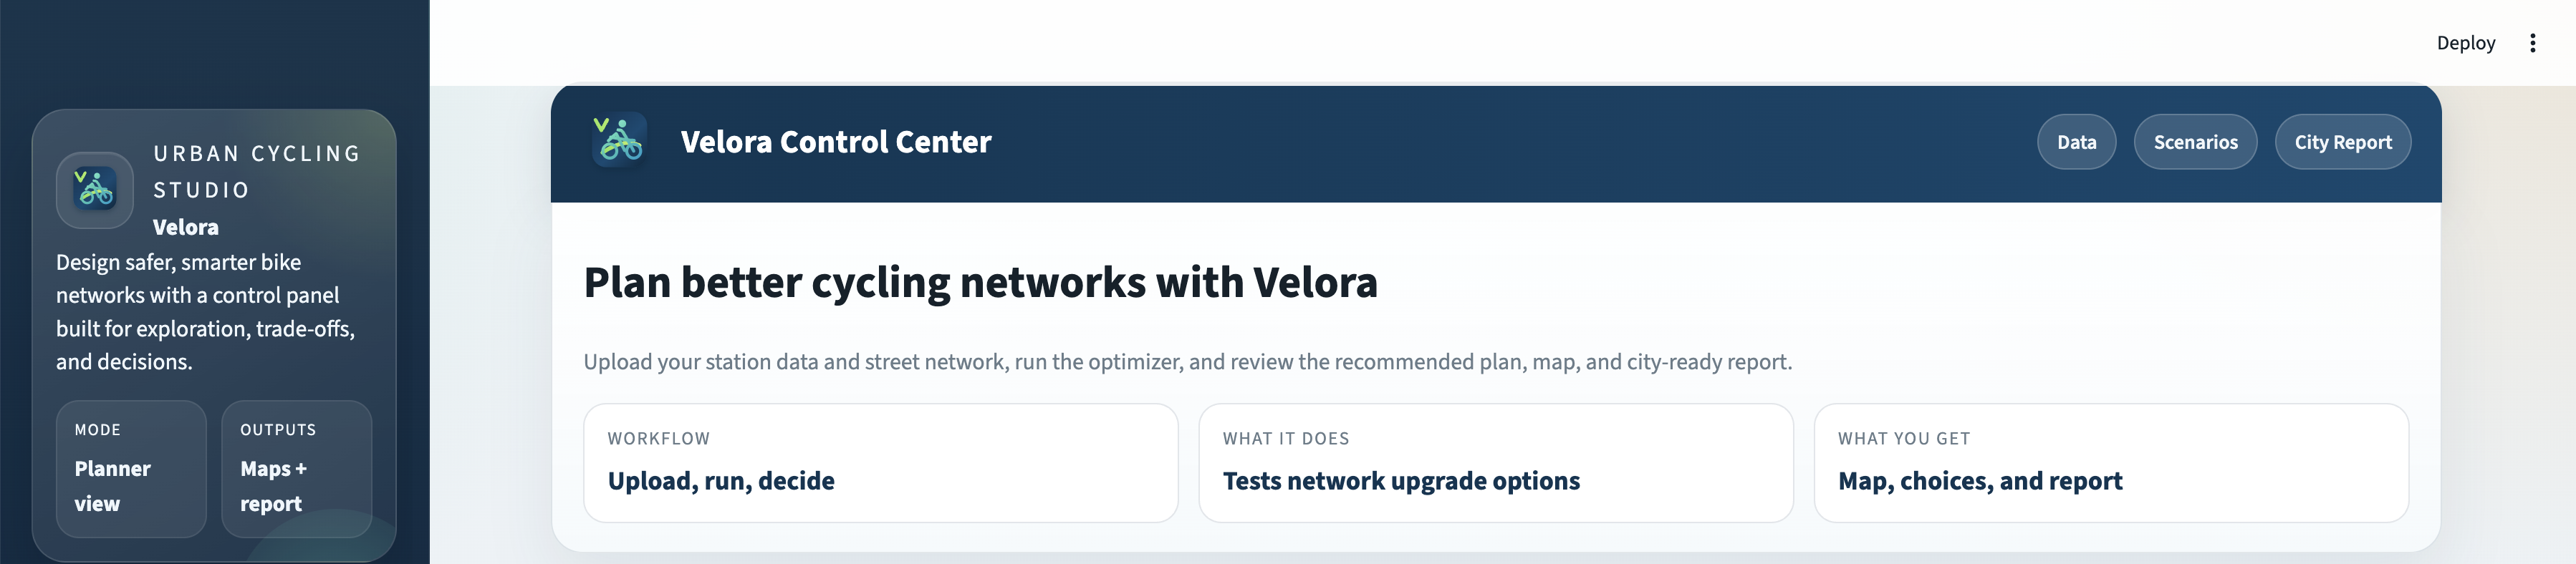
\includegraphics[width=\textwidth]{Figures/velora_control_center.png}
  \caption{Velora control center showing the data, scenario, and city-report workflow.}
  \label{fig:velora_control_center}
\end{figure}

\subsection{Modules and User Experience}

The user experience is structured around four main screens or functional areas:

\begin{enumerate}
    \item \textbf{Input configuration:} Users provide station and network files, specify the back-end connection, and define the study area and candidate-generation settings.
    \item \textbf{Planning assumptions:} Users set policy and model parameters, including minimum stations, minimum links, demand thresholds, dock costs, station fixed costs, link upgrade costs by LTS class, population size, generations, mutation probability, and random seed.
    \item \textbf{Optimization results:} Users review the approximated Pareto set and compare representative solutions, including balanced, best-demand, best-stress, and best-cost scenarios.
    \item \textbf{Scenario archive and reporting:} Users reopen saved runs, inspect previous outputs, export station and link recommendations, and generate summary reports for external review.
\end{enumerate}

Table~\ref{tab:velora_ux} summarizes the relationship between platform actions and decision-making tasks.

\begin{table}[htbp]
  \centering
  \caption{Velora user-experience elements and decision-making roles.}
  \label{tab:velora_ux}
  \small
  \begin{tabularx}{0.95\textwidth}{@{} l X X @{}}
    \hline
    \textbf{UX element} & \textbf{User action} & \textbf{Decision-making role} \\
    \hline
    File upload controls & Import station demand and LTS network layers. & Ensures that planning scenarios use transparent, locally relevant data. \\
    Parameter controls & Adjust service thresholds, costs, buffers, and algorithm settings. & Converts policy assumptions into explicit model parameters. \\
    Scenario metrics & Compare demand, average LTS, cost, selected stations, and selected links. & Supports rapid screening of alternatives. \\
    Interactive maps & Inspect selected stations, candidate locations, and recommended link upgrades. & Helps planners identify implementable corridors and spatial conflicts. \\
    Saved runs & Reopen and compare previous experiments. & Creates an auditable record of planning assumptions and results. \\
    Report generator & Produce city-ready summaries of selected scenarios. & Converts technical optimization results into material for policy review and stakeholder communication. \\
    Exportable outputs & Download selected stations, links, Pareto rows, report material, and map artifacts. & Supports transfer to GIS, reporting, and stakeholder review. \\
    \hline
  \end{tabularx}
\end{table}

\subsection{Representative Platform Outputs}

Figures~\ref{fig:velora_tradeoff_screen}--\ref{fig:velora_appendix_solution} illustrate outputs that Velora exposes to users after an optimization run. These figures correspond to the same decision objects used in the main analysis: Pareto trade-offs, mapped representative scenarios, and sensitivity results. In the platform, these outputs are paired with interactive controls, downloadable station/link tables, and report-generation tools.

\begin{figure}[htbp]
  \centering
  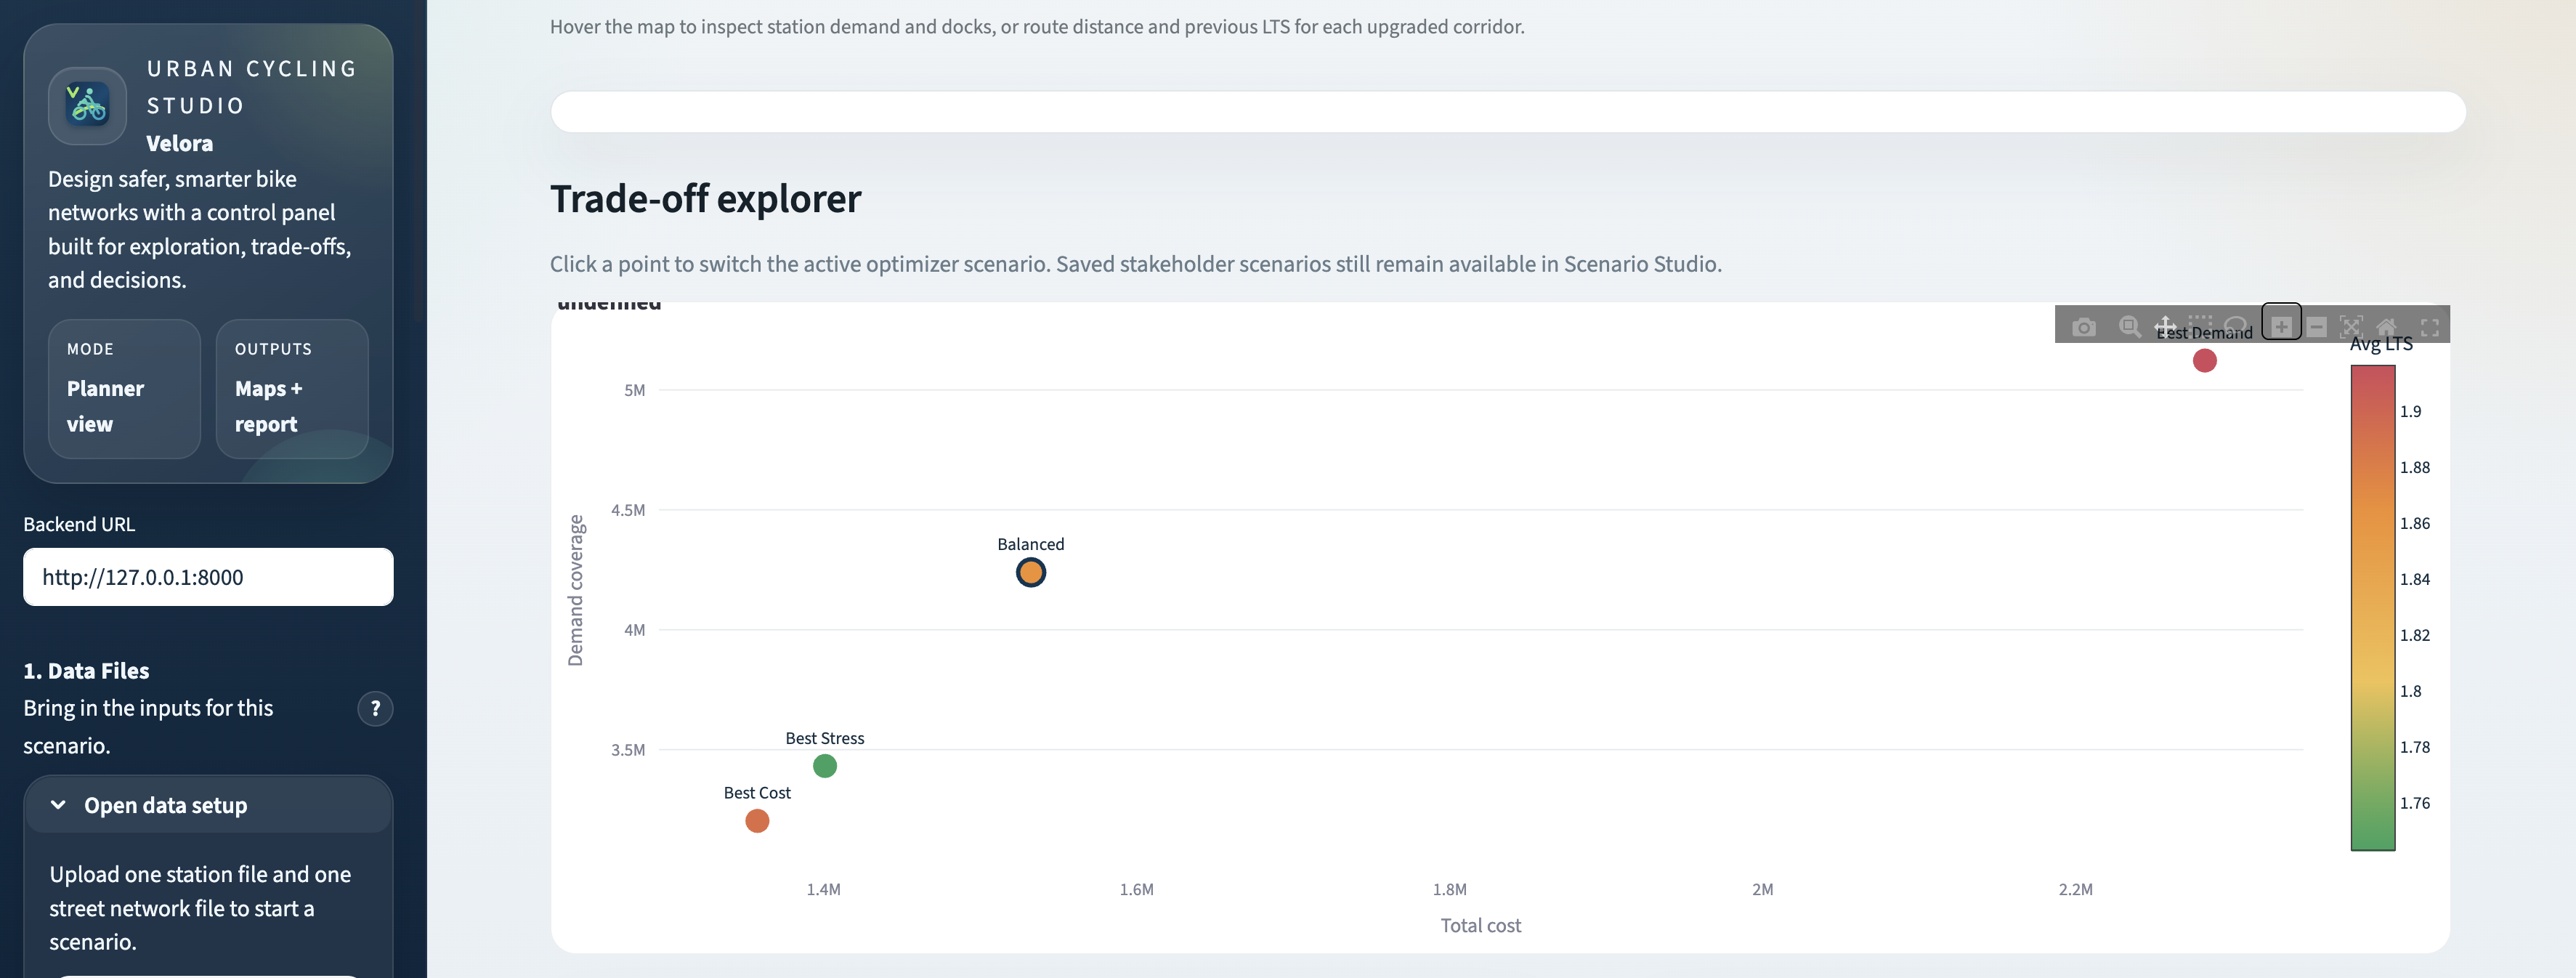
\includegraphics[width=\textwidth]{Figures/velora_tradeoff_explorer.png}
  \caption{Velora trade-off explorer, where users compare demand coverage, cost, and average LTS across alternative scenarios.}
  \label{fig:velora_tradeoff_screen}
\end{figure}

\begin{figure}[htbp]
  \centering
  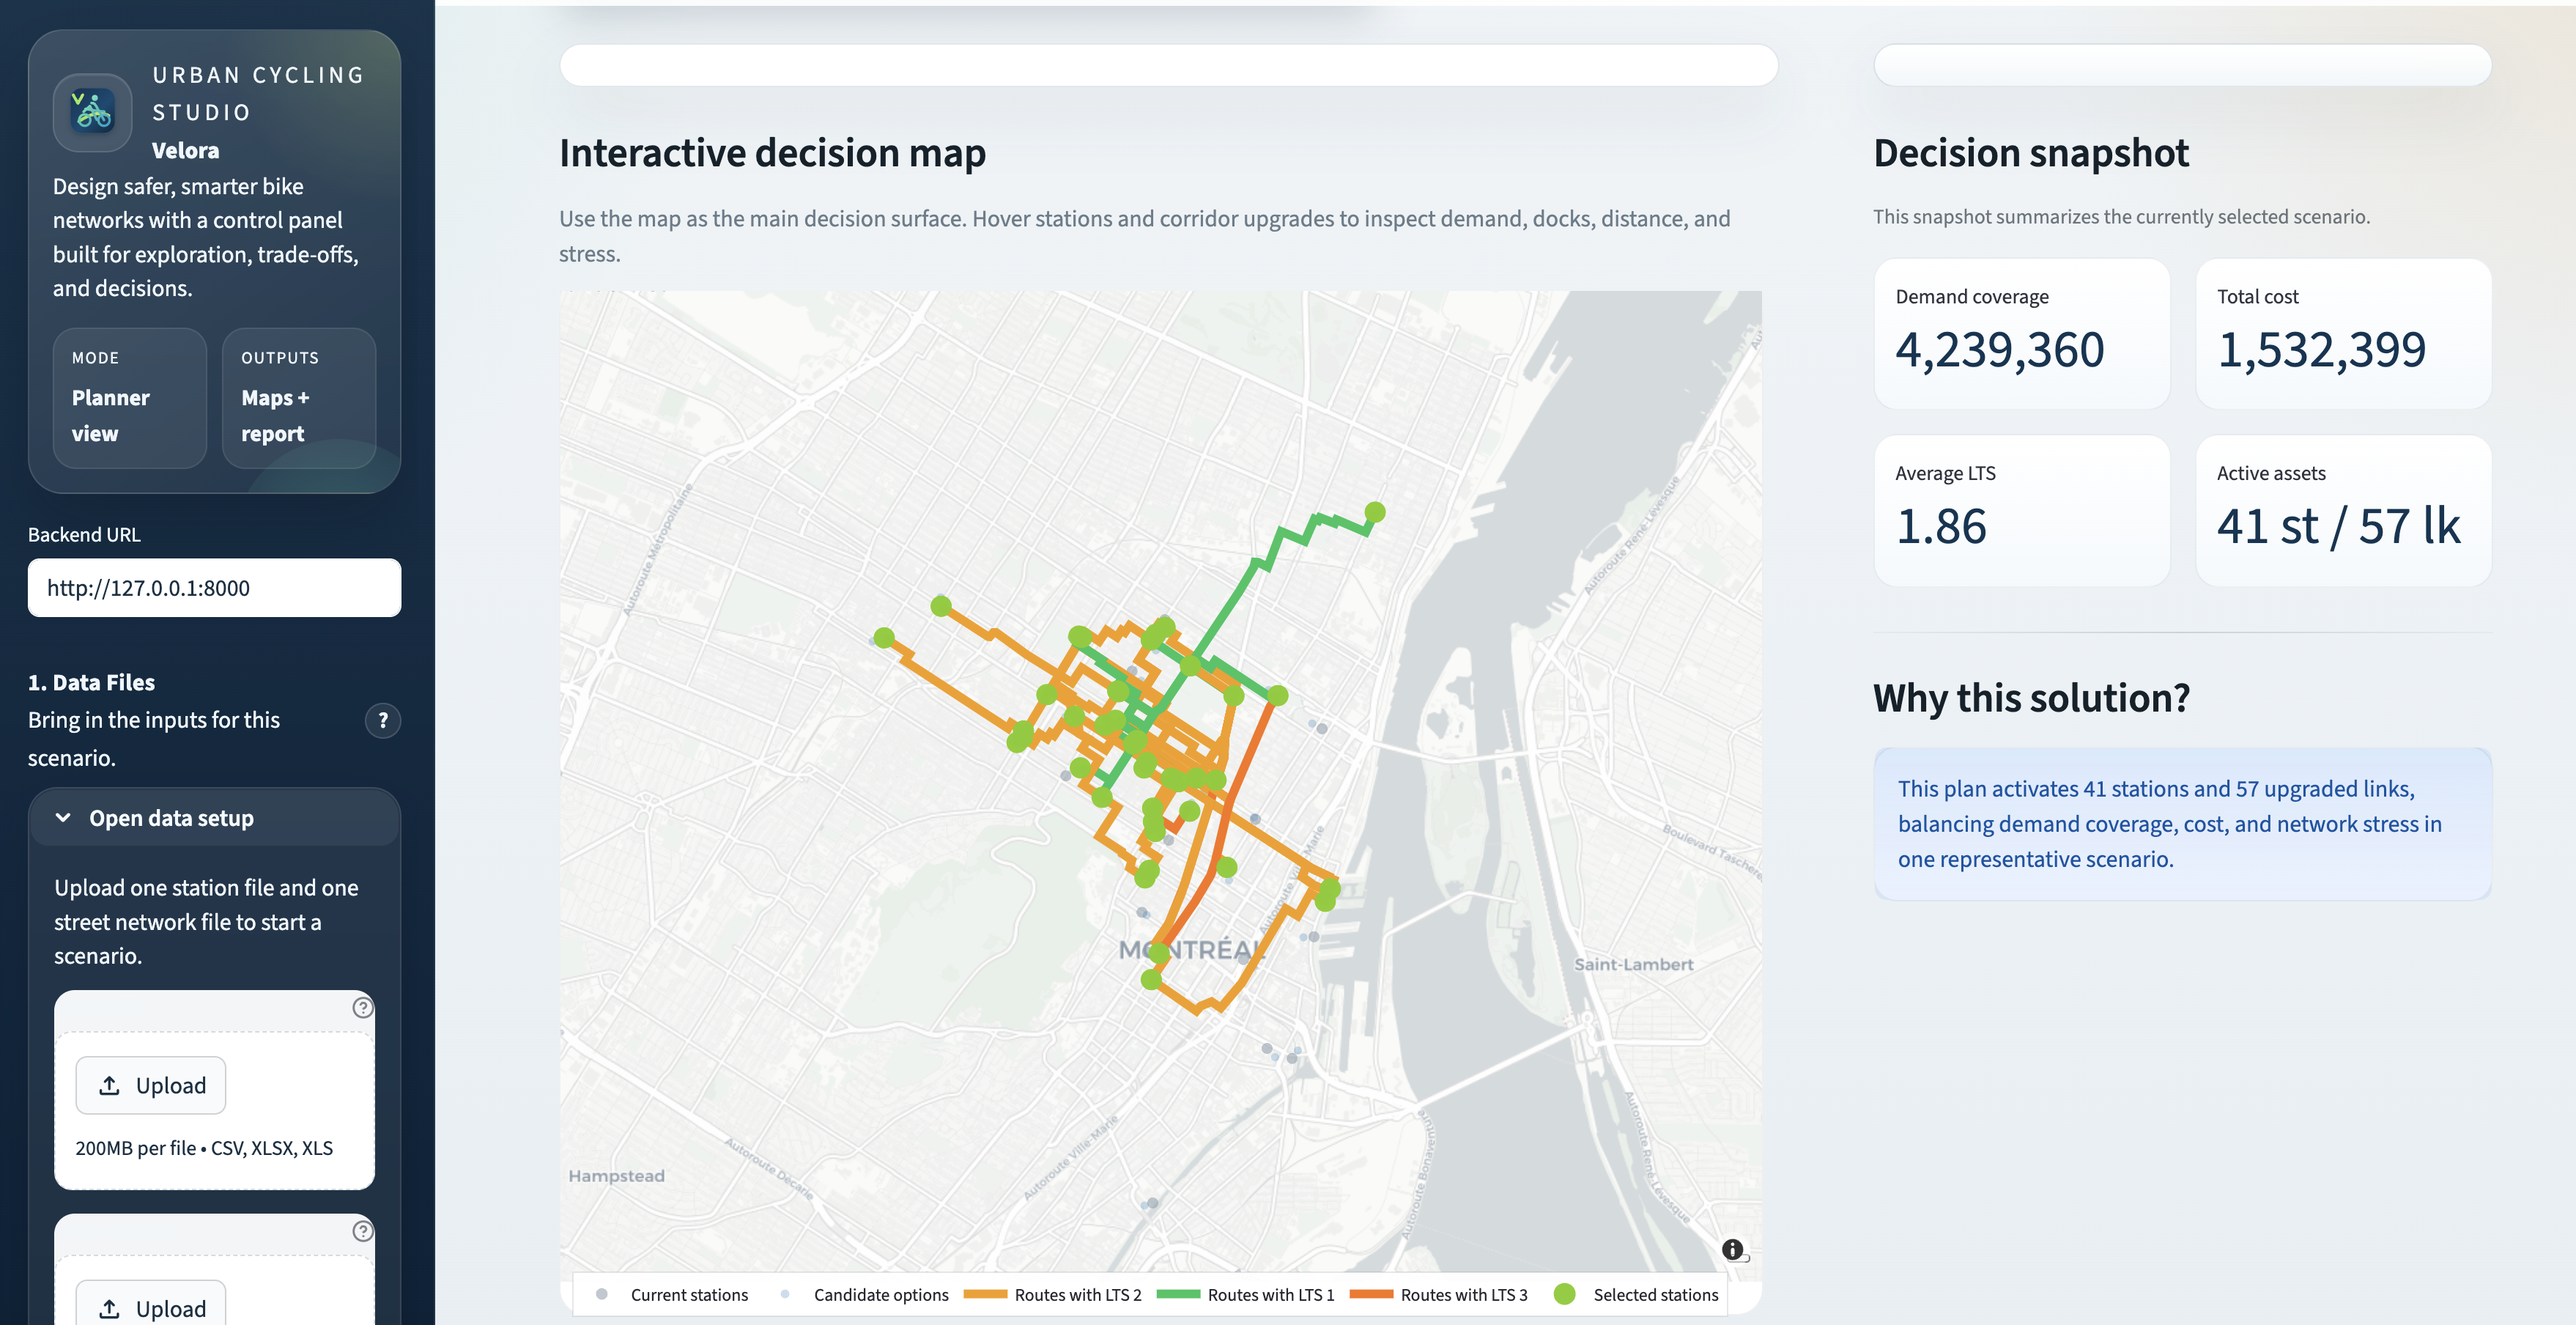
\includegraphics[width=\textwidth]{Figures/velora_decision_map.png}
  \caption{Velora interactive decision map and scenario snapshot showing selected stations, upgraded links, demand coverage, cost, average LTS, and active assets.}
  \label{fig:velora_decision_map_screen}
\end{figure}

\begin{figure}[htbp]
  \centering
  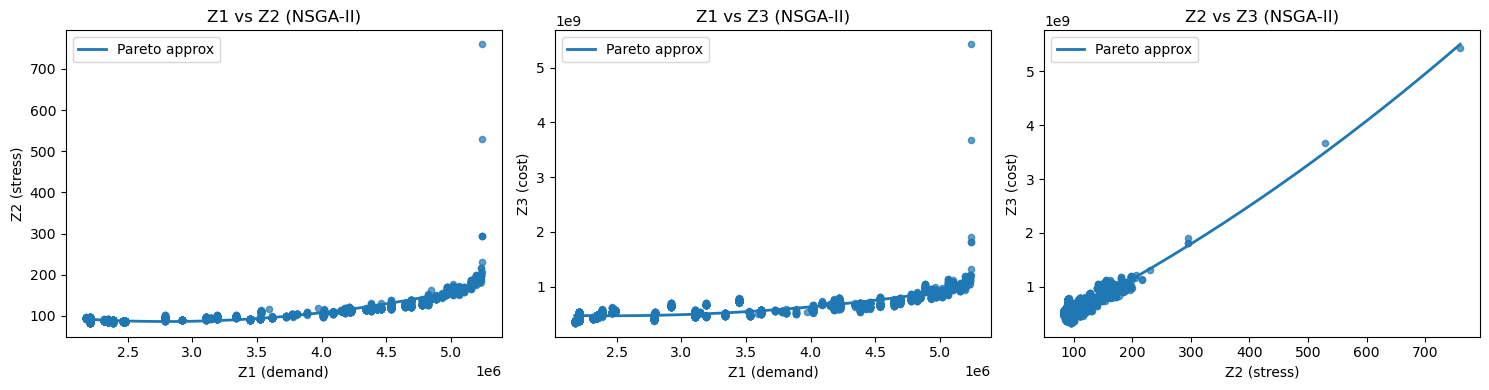
\includegraphics[width=\textwidth]{Figures/Plots_2D_Pop_3000_Gen_100.png}
  \caption{Representative Velora Pareto-view output showing pairwise trade-offs among demand coverage, LTS, and investment cost.}
  \label{fig:velora_appendix_pareto}
\end{figure}

\begin{figure}[htbp]
    \centering
    \begin{subfigure}[b]{0.48\textwidth}
        \centering
        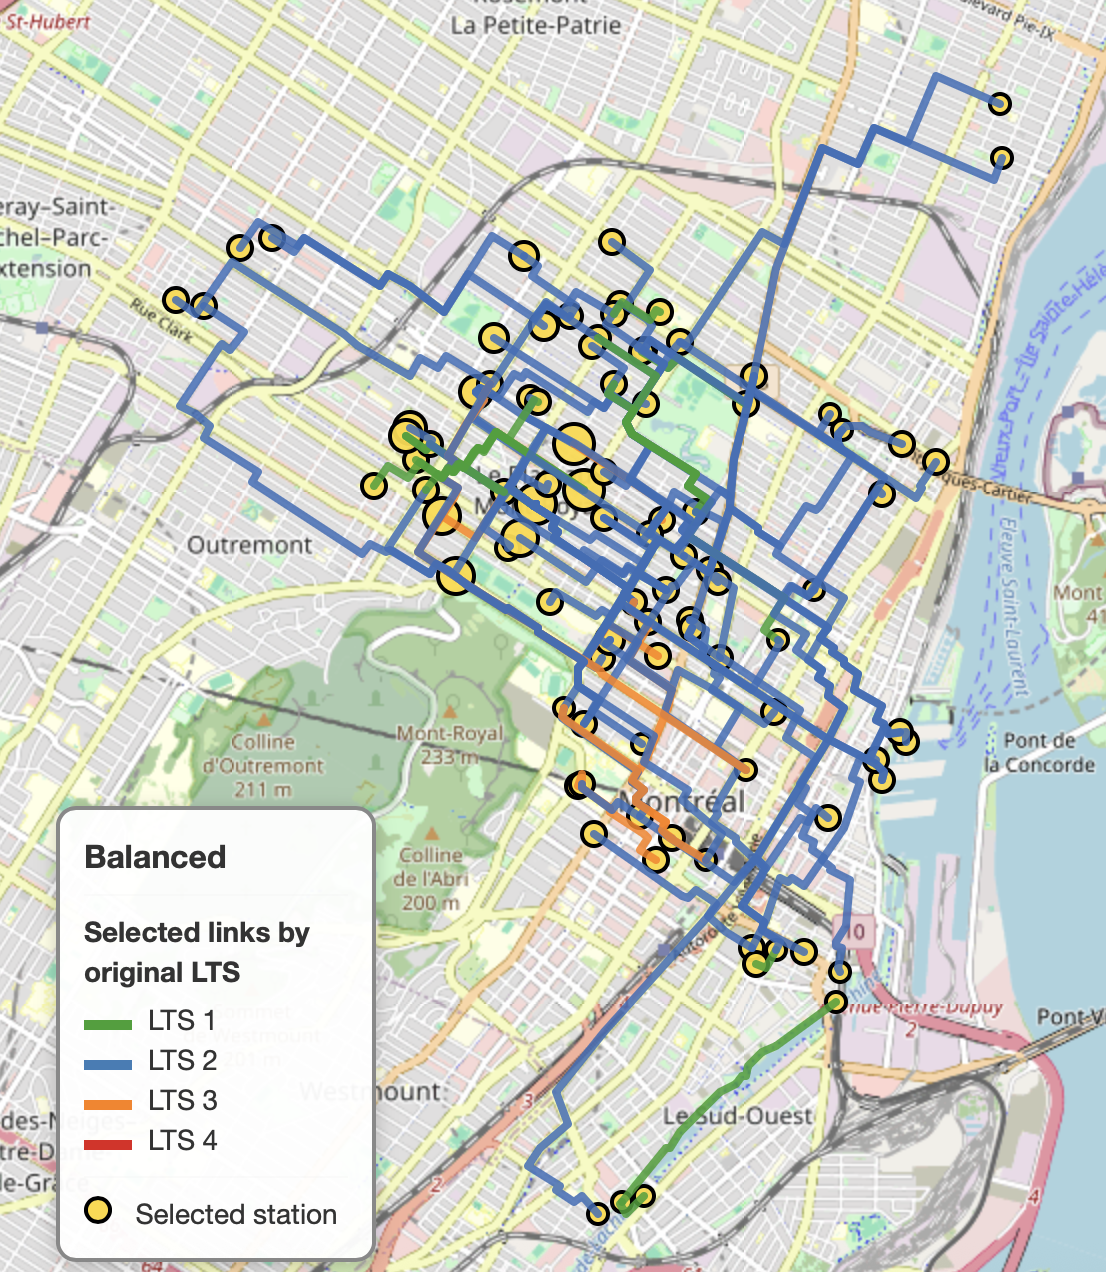
\includegraphics[width=\textwidth]{Figures/nsga_Balanced_Solution_map_3000_100.png}
        \caption{Balanced scenario.}
    \end{subfigure}
    \hfill
    \begin{subfigure}[b]{0.48\textwidth}
        \centering
        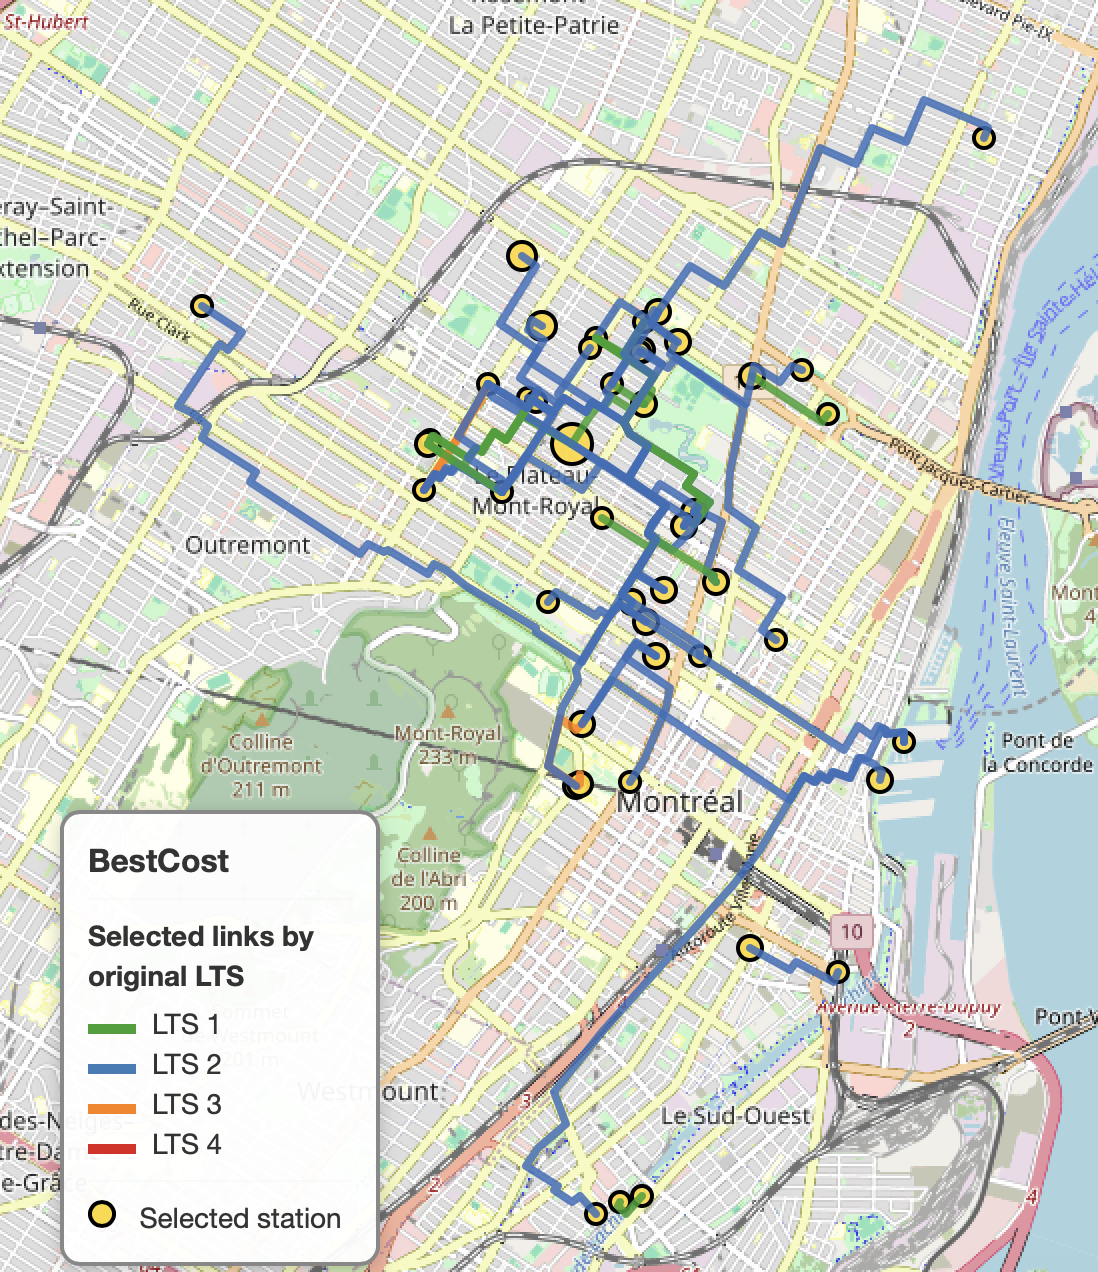
\includegraphics[width=\textwidth]{Figures/nsga_Best_Cost_map_3000_100.png}
        \caption{Best-cost scenario.}
    \end{subfigure}
    \caption{Representative Velora map outputs used to compare spatial implications of alternative investment priorities.}
    \label{fig:velora_appendix_solution}
\end{figure}

\subsection{Implementation Notes}

The current Velora implementation stores runs under a persistent run directory, with each run containing configuration metadata, selected station and link tables, Pareto rows, map-ready artifacts, and report-ready summaries. The front-end presents the planner with a compact interface for running new scenarios and reopening completed ones. The optimization module uses geospatial processing to generate candidate stations, construct graph-based link alternatives, evaluate stress and cost, and select representative scenarios from the Pareto set. This modular structure allows the platform to be extended with additional planning objectives, such as equity, public-transit access, emissions impacts, maintenance constraints, or automated reporting templates for different municipal departments, without altering the basic workflow.

\setcounter{figure}{0}
\setcounter{table}{0}
\section{BIXI Stations Demand}\label{app:top30_stations}

Table~\ref{tab:top30_station_activity} reports the 30 downtown BIXI stations used to define the computational study area, ranked by annual station activity in the 2025 dataset. Activity is measured as the sum of departures and arrivals at each station.

\setlength{\LTleft}{0pt}
\setlength{\LTright}{0pt}
\small
\begin{longtable}{@{}p{0.08\textwidth} p{0.62\textwidth} p{0.16\textwidth}@{}}
\caption{Top 30 downtown BIXI stations by annual activity.}\label{tab:top30_station_activity}\\
\hline
\textbf{Rank} & \textbf{Station} & \textbf{Annual activity} \\
\hline
\endfirsthead

\multicolumn{3}{@{}l}{\tablename\ \thetable\ -- continued from previous page}\\
\hline
\textbf{Rank} & \textbf{Station} & \textbf{Annual activity} \\
\hline
\endhead

\hline
\multicolumn{3}{r@{}}{Continued on next page}\\
\endfoot

\hline
\endlastfoot
1 & Métro Mont-Royal (Utilités publiques / Rivard) & 245,460 \\
2 & du Mont-Royal / Clark & 228,292 \\
3 & Laurier / St-Denis & 171,054 \\
4 & Laurier / de Brébeuf & 149,403 \\
5 & des Pins / St-Laurent & 141,754 \\
6 & de la Commune / Place Jacques-Cartier & 131,337 \\
7 & Métro Peel (de Maisonneuve / Stanley) & 131,261 \\
8 & Métro St-Laurent (de Maisonneuve / St-Laurent) & 121,207 \\
9 & McTavish / Sherbrooke & 118,148 \\
10 & Prince-Arthur / du Parc & 115,810 \\
11 & Ottawa / Young & 113,831 \\
12 & Clark / Laurier & 111,426 \\
13 & Berri / Rachel & 111,097 \\
14 & Métro Papineau (Dorion / De Maisonneuve) & 110,895 \\
15 & Émile-Duployé / Sherbrooke & 108,685 \\
16 & de la Commune / St-Sulpice & 104,983 \\
17 & Clark / Prince-Arthur & 101,935 \\
18 & de Châteaubriand / Beaubien & 98,850 \\
19 & Émile-Duployé / Rachel & 97,449 \\
20 & Métro Sherbrooke (de Rigaud / Berri) & 95,487 \\
21 & Marquette / du Mont-Royal (sud) & 93,378 \\
22 & Marquette / du Mont-Royal & 92,237 \\
23 & Roy / St-Denis & 91,825 \\
24 & Smith / Peel & 91,150 \\
25 & Boyer / du Mont-Royal & 89,800 \\
26 & Charles-Biddle / Atwater & 89,786 \\
27 & Duluth / St-Denis & 89,669 \\
28 & Aylwin / Ontario & 89,014 \\
29 & Berri / de Maisonneuve & 86,820 \\
30 & University / Milton & 86,802 \\
\end{longtable}
\normalsize

\setcounter{figure}{0}
\setcounter{table}{0}

\section{Sensitivity Analysis Supplementary Material}\label{app:sensitivity_details}

This appendix reports the full-value sensitivity tables and Pareto-front projections corresponding to the normalized discussion in Section~\ref{results}. These materials are provided for completeness and cross-checking, while the interpretation in the main text relies on normalized metrics. Table~\ref{tab:sensitivity_smin} reports the absolute objective values obtained under different minimum station constraints, allowing direct comparison with the normalized results.

\begin{table}[htb]
  \caption{Sensitivity analysis results for different minimum station constraints ($S_{\min}$).}
  \label{tab:sensitivity_smin}
  \centering
  \small
  \begin{tabular}{@{}lcccc@{}}
    \hline
    \textbf{$S_{\min}$} & \textbf{30} & \textbf{40} & \textbf{50} & \textbf{60} \\
    \hline
    Max Z1 (million) & 4.557 & 4.560 & 4.583 & 4.663 \\
    Min Z2 & 38.67 & 45.45 & 57.58 & 67.56 \\
    Min Z3 (million) & 3.06 & 3.09 & 3.18 & 4.48 \\
    \hline
  \end{tabular}
\end{table}

Figure~\ref{fig:Sen_pareto_2d} illustrates how the Pareto front shifts in objective space as station requirements become more restrictive.

\begin{figure}[htbp]
  \centering
  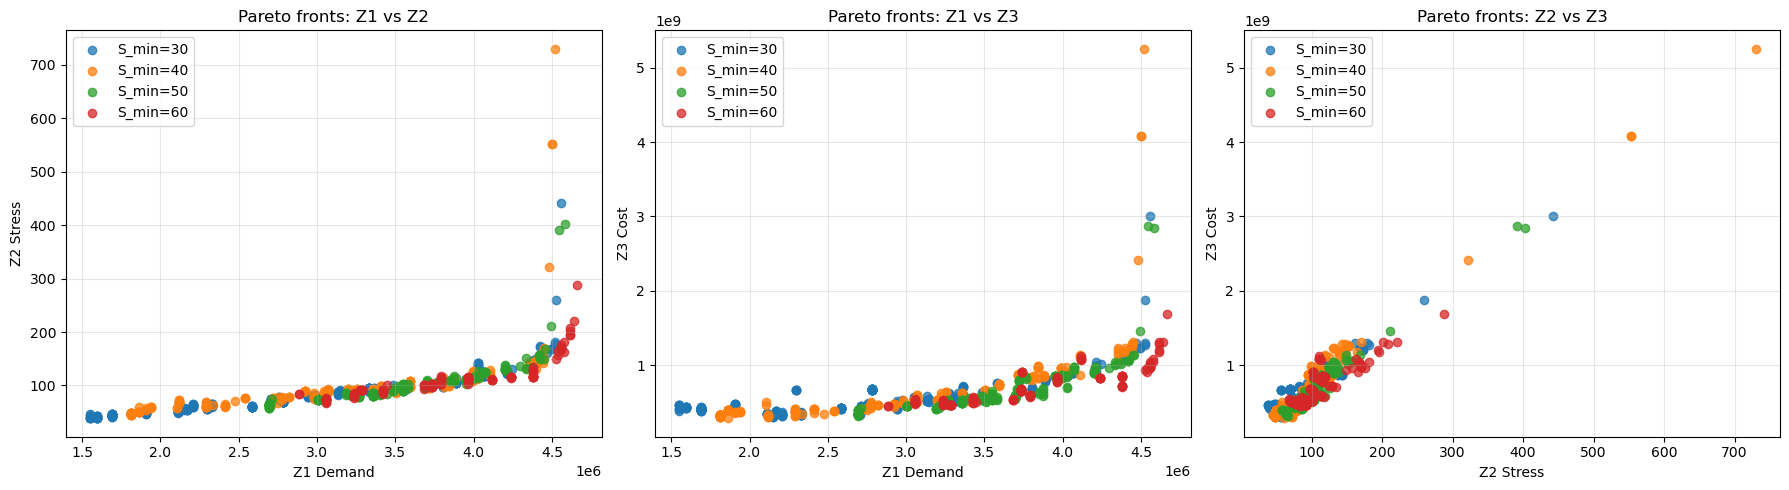
\includegraphics[width=\textwidth]{Figures/Sensitivity_Plots_2D_Pop_1200_V3.png}
  \caption{Pairwise projections of the NSGA-II Pareto set showing sensitivity to the minimum number of stations.}
  \label{fig:Sen_pareto_2d}
\end{figure}

Table~\ref{tab:sensitivity_mmin} presents the corresponding absolute results for varying minimum link constraints, highlighting their impact on demand, stress, and cost.

\begin{table}[htbp]
  \caption{Sensitivity analysis results for different minimum link constraints ($M_{\min}$).}
  \label{tab:sensitivity_mmin}
  \centering
  \small
  \begin{tabular}{@{}lcccc@{}}
    \hline
    \textbf{$M_{\min}$} & \textbf{50} & \textbf{100} & \textbf{150} & \textbf{200} \\
    \hline
    Max Z1 (million) & 4.953 & 4.851 & 4.711 & 4.820 \\
    Min Z2 & 87.19 & 158.39 & 247.92 & 330.80 \\
    Min Z3 (million) & 5.24 & 8.65 & 12.95 & 16.37 \\
    \hline
  \end{tabular}
\end{table}

Figure~\ref{fig:Sen_pareto_2d_links} shows the evolution of the Pareto front as link requirements increase, highlighting changes in trade-offs among objectives.

\begin{figure}[htbp]
  \centering
  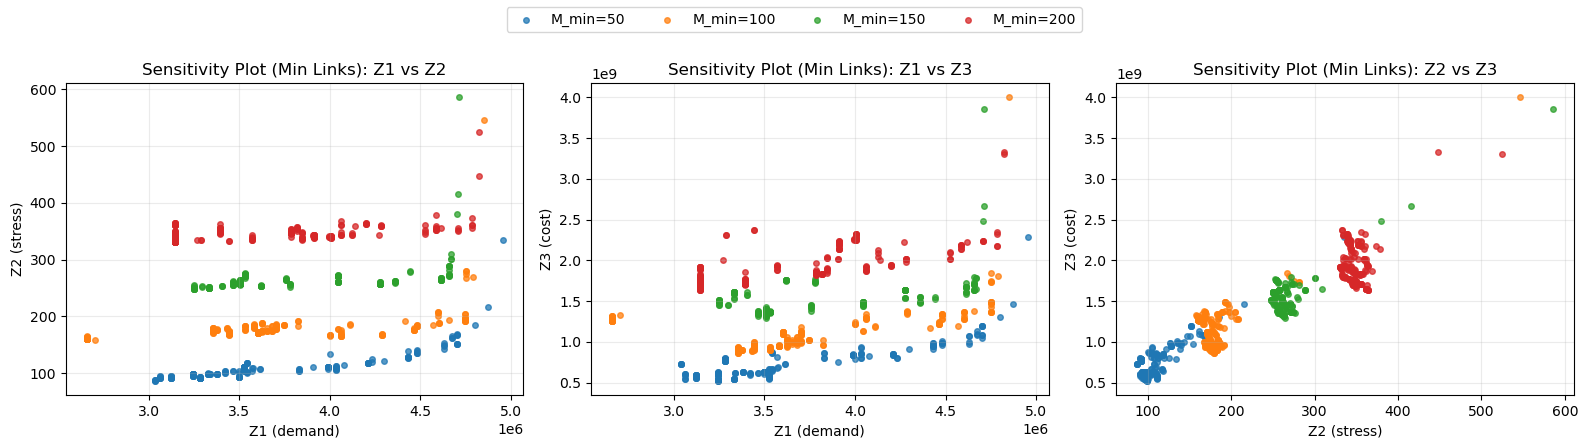
\includegraphics[width=\textwidth]{Figures/Sensitivity_Links_Plots_2D_Pop_1200.png}
  \caption{Pairwise projections of the NSGA-II Pareto set showing sensitivity to the minimum number of links.}
  \label{fig:Sen_pareto_2d_links}
\end{figure}

% =================== Statements ===================
\section*{CRediT authorship contribution statement}
\textbf{Conceptualization:} NA, JAM, JY, LMM. 
\textbf{Methodology:} NA, JAM, JY, LMM. 
\textbf{Data curation:} NA. 
\textbf{Formal analysis:} NA, JAM. 
\textbf{Software:} NA. 
\textbf{Visualization:} NA. 
\textbf{Writing -- original draft:} NA, JAM. 
\textbf{Writing -- review \& editing:} NA, JAM, JY, LMM. 
\textbf{Supervision:} JY, LMM. 
\textbf{Funding acquisition:} LMM.

\section*{Declaration of competing interest}
The authors declare that they have no known competing financial interests or personal relationships that could have appeared to influence the work reported in this paper.

\section*{Funding}
This work was supported by Environment and Climate Change Canada (ECCC), the New Frontiers in Research Fund (NFRF, Exploration Grant), and the Fonds de recherche du Québec (FRQ, AUDACE Grant). The funders had no role in the study design, data processing, analysis, interpretation of results, manuscript preparation, or decision to submit the article for publication.

\section*{Data availability}
The BIXI trip data used in this study are publicly available through BIXI Montreal open data at \url{https://bixi.com/en/open-data/}. The derived LTS network, optimization instances, and platform outputs contain processed geospatial layers and will be made available by the corresponding author upon reasonable request, subject to data-use and licensing constraints.

\section*{Acknowledgments}
The authors thank the data providers and municipal open-data programs that made the empirical cycling and geospatial inputs available for this study.

% References are now handled by the elsarticle class
% The bibstyle is changed to elsarticle-num
\bibliographystyle{elsarticle-harv}
\bibliography{refs}
% References
\end{document}
